\documentclass[a4paper,12pt]{report}


\usepackage[utf8]{inputenc}
\usepackage{babel}
\usepackage[T1]{fontenc}
\usepackage[a4paper,margin=2cm]{geometry} % margins (replaces anysize)

%%%%%%%% Preamble %%%%%%%%%%%%
\usepackage[hidelinks]{hyperref}
\usepackage[utf8]{inputenc} % File coding uses utf8
\usepackage{amsmath} % Extra commands for math
\usepackage{amssymb} % Math symbols
\usepackage{graphicx} % Include images in LaTeX
\usepackage{color} % Coloring text
\usepackage{float} % Allow you to use [H] specifier to force the position of the images
\usepackage{caption} % to customize the captions in floating environments like figure and table




%webography
\usepackage[natbib=true,style=numeric,sorting=none]{biblatex}
\addbibresource{bib/webography.bib}
\renewcommand\bibname{Webography}

% webography to remove italic and stuff

\makeatletter
\renewrobustcmd*{\mkbibemph}{}
\protected\long\def\blx@imc@mkbibemph#1{#1}
\makeatother

% Header and Footer
\usepackage{fancyhdr}
\pagestyle{fancy}

\renewcommand{\chaptermark}[1]{\markboth{\MakeUppercase{\thechapter: #1}}{}}
\fancyhead[L]{CHAPTER \leftmark}
\fancyhead[R]{}



%\fancyhead[L]{\footnotesize Higher Institute of Technological Studies in Communications of Tunis}
%\fancyhead[R]{\footnotesize Year 2025-2026}
%\fancyfoot[C]{\thepage}  % center


\renewcommand{\headrulewidth}{0.25pt} % remove the header line
\renewcommand{\footrulewidth}{0pt} % remove the footer line

\usepackage{listings} % To use source code
\definecolor{dkgreen}{rgb}{0,0.6,0} % Color for using code
\definecolor{gray}{rgb}{0.5,0.5,0.5}
% Language to use
\lstset{language=Python,
   keywords={break,case,catch,continue,else,elseif,end,for,function,
      global,if,otherwise,persistent,return,switch,try,while,async,await,class,def,import,from},
   basicstyle=\ttfamily\footnotesize,
   keywordstyle=\color{blue},
   commentstyle=\color{red},
   stringstyle=\color{dkgreen},
   numbers=left,
   numberstyle=\tiny\color{gray},
   stepnumber=1,
   numbersep=10pt,
   backgroundcolor=\color{white},
   tabsize=4,
   showspaces=false,
   showstringspaces=false}

\title{Degree project}

\setcounter{secnumdepth}{4}
\setcounter{tocdepth}{4}
\setcounter{chapter}{0}
\graphicspath{ {./images/} }


%%%%%%%%%%%%%%%%%%%%%%%%%%%%%%%%%%%%%%%%%%%%%%%%%%%%%%%%%%%%%%%%%%%%%%%%%%
% for table of contents spacing

% for table of figures
\linespread{1.25}
%%%%%%%%%%%%%%%%%%%%%%%%%%%%%%%%%%%%%%%%%%%%%%%%%%%%%%%%%%%%%%%%%%%%%%%%%%

\usepackage{acronym}

\pagenumbering{roman}
\begin{document}
%%%%%%%%%%%%%%%%%%%%%%%%%%%%%%%%%%%%%%%%%%%%%%%%%%%%%%%%%%%%%%%%%%%%%%%%%%

% =====================================================================
% NOTE: The institutional cover page / title page provided by the
% school template should be placed here (e.g. \includepdf{cover.pdf}).
% It is intentionally omitted so it can be added without conflict.
% =====================================================================

\newpage
\chapter*{Acknowledgement}

First, we would like to thank everyone who, in one way or another, contributed to the completion of this project. We are especially grateful to the open threat-intelligence community, whose freely shared feeds, standards, and tooling, MITRE ATT\&CK, abuse.ch, CISA, and the FIRST.org EPSS effort among them, made an integrative platform such as ours possible in the first place.\hfill\break

Second, we would like to express our gratitude to our academic supervisors for their invaluable guidance and support throughout the design and development of our Threat Intelligence Platform. Their knowledge and expertise were instrumental in helping us navigate the complexities of distributed systems design, secure software architecture, and the responsible application of large language models to security analysis. This project would not have been successful without their cooperation and insights.\hfill\break

We also extend our sincere thanks to our host organization for welcoming us, framing a problem worth solving, and giving us the operational context that shaped every design decision in this work.\hfill\break

Finally, we would like to express our deepest appreciation to our families for their unwavering support throughout this journey. Their encouragement and presence have been a constant source of motivation and strength.
\hfill\break

%%%%%%%%%%%%%%%%%%%%%%%%%%%%%%%%%%%%%%%%%%%%%%%%%%%%%%%%%%%%%%%%%%%%%%%%%%
\newpage
\chapter*{Acronyms}
\begin{acronym}[aaaaaaaaaa]\itemsep=-5pt % Give the longest label here so that the list is nicely aligned
\acro{API}{Application Programming Interface}
\acro{APT}{Advanced Persistent Threat}
\acro{ASM}{Attack Surface Management}
\acro{ATTACK}[ATT\&CK]{Adversarial Tactics, Techniques, and Common Knowledge}
\acro{BFF}{Backend For Frontend}
\acro{CI/CD}{Continuous Integration and Continuous Delivery}
\acro{CIDR}{Classless Inter-Domain Routing}
\acro{CLI}{Command Line Interface}
\acro{CORS}{Cross-Origin Resource Sharing}
\acro{CPE}{Common Platform Enumeration}
\acro{CT}{Certificate Transparency}
\acro{CTI}{Cyber Threat Intelligence}
\acro{CVE}{Common Vulnerabilities and Exposures}
\acro{CVSS}{Common Vulnerability Scoring System}
\acro{DNS}{Domain Name System}
\acro{DTO}{Data Transfer Object}
\acro{EPSS}{Exploit Prediction Scoring System}
\acro{HIBP}{Have I Been Pwned}
\acro{HTTP}{Hypertext Transfer Protocol}
\acro{IAM}{Identity and Access Management}
\acro{IOC}{Indicator of Compromise}
\acro{IP}{Internet Protocol}
\acro{JSON}{JavaScript Object Notation}
\acro{JWT}{JSON Web Token}
\acro{KEV}{Known Exploited Vulnerabilities}
\acro{LLM}{Large Language Model}
\acro{MFA}{Multi-Factor Authentication}
\acro{MISP}{Malware Information Sharing Platform}
\acro{PAT}{Personal Access Token}
\acro{NVD}{National Vulnerability Database}
\acro{ORM}{Object-Relational Mapping}
\acro{OSINT}{Open Source Intelligence}
\acro{RBAC}{Role-Based Access Control}
\acro{REST}{Representational State Transfer}
\acro{RSS}{Really Simple Syndication}
\acro{SIEM}{Security Information and Event Management}
\acro{SOC}{Security Operations Centre}
\acro{SQL}{Structured Query Language}
\acro{SSE}{Server-Sent Events}
\acro{SaaS}{Software as a Service}
\acro{SSL}{Secure Sockets Layer}
\acro{STIX}{Structured Threat Information eXpression}
\acro{TLS}{Transport Layer Security}
\acro{TIP}{Threat Intelligence Platform}
\acro{TTP}{Tactics, Techniques and Procedures}
\acro{UML}{Unified Modeling Language}
\acro{UUID}{Universally Unique Identifier}
\end{acronym}


%%%%%%%%%%%%%%%%%%%%%%%%%%%%%%%%%%%%%%%%%%%%%%%%%%%%%%%%%%%%%%%%%%%%%%%%%%
\newpage



%%%%%%%%%%%%%%%%%%%%%%%%%%%%%%%%%%%%%%%%%%%%%%%%%%%%%%%%%%%%%%%%%%%%%%%%%%

\tableofcontents
\clearpage
\thispagestyle{plain}


%%%%%%%%%%%%%%%%%%%%%%%%%%%%%%%%%%%%%%%%%%%%%%%%%%%%%%%%%%%%%%%%%%%%%%%%%%
\newpage
\listoffigures
%%%%%%%%%%%%%%%%%%%%%%%%%%%%%%%%%%%%%%%%%%%%%%%%%%%%%%%%%%%%%%%%%%%%%%%%%%
\newpage
\listoftables

%%%%%%%%%%%%%%%%%%%%%%%%%%%%%%%%%%%%%%%%%%%%%%%%%%%%%%%%%%%%%%%%%%%%%%%%%%
%%%%%%%%%%%%%%%%%%%%%%%%%%%%%%%%%%%%%%%%%%%%%%%%%%%%%%%%%%%%%%%%%%%%%%%%%%
\newpage
\pagenumbering{arabic}
\chapter*{General Introduction}
\addcontentsline{toc}{chapter}{General Introduction}

Security operations now take place under a form of time compression that did not exist a few years ago. Vulnerabilities are disclosed at high volume, proof-of-concept code appears quickly, cloud and SaaS identities have become privileged attack surfaces, and threat actors increasingly automate reconnaissance, credential theft, and social engineering. The limiting factor for many teams is no longer access to raw security data; it is the ability to correlate heterogeneous signals quickly enough to reach a defensible decision before conditions change again. Reports from CrowdStrike, Unit 42, Sophos, GitHub, Wiz, and CISA all point in the same direction: the operational window available to defenders has narrowed, while the number of relevant signals has expanded \cite{crowdstrike_gtr_2026,unit42_ir_2026,sophos_threat_2025,github_oss_trends_2026,wiz_ai_readiness_2026,cisa_kev}.

The platform studied in this report was engineered for that environment. It is a self-hosted Threat Intelligence Platform (TIP) designed for a small security organization that needs one working system rather than a collection of disconnected products. The implementation combines fifteen FastAPI services, nine shared Python packages, a Next.js frontend with a backend-for-frontend proxy, PostgreSQL behind PgBouncer, Redis, a LiteLLM gateway, and a scheduler-driven execution model. Its purpose is not to collect threat data for its own sake. Its purpose is to reduce the distance between raw intelligence and operational judgment: which vulnerabilities matter to this organization, which threat actors are plausible, which indicators deserve attention now, and what should an analyst or manager do next.

Several architectural decisions follow directly from that operational objective. Intelligence ingestion is separated from AI-driven synthesis so that data collection survives model outages and quota exhaustion. Services own their schemas and communicate through HTTP rather than shared table access, which preserves modularity even within a single-host deployment. Secrets are centralized, outbound calls are wrapped in a resilience layer, and the latency-critical indicator lookup path is cached aggressively. The implementation therefore reflects a specific engineering stance: availability, traceability, and operability matter at least as much as algorithmic sophistication.

This report rebuilds the project narrative from the implementation upward. It does not treat the source code as an appendix to a design story written in advance. Instead, the architecture, workflows, trust boundaries, deployment model, testing posture, and operational tradeoffs are derived from the repository and its infrastructure. The first chapter situates the work in the modern threat landscape and explains why partially automated, AI-assisted security operations have become operationally necessary. The second establishes the theoretical foundations required to understand the project properly. The third positions the work against existing solutions. The fourth explains the methodology and engineering process through which the system was analysed and built. The fifth translates the problem context into requirements and design constraints. The sixth explains the architecture of the delivered system. The seventh clarifies the infrastructure stack and platform technologies in detail. The eighth introduces the service catalogue and capability map. The ninth deepens that view with a service-by-service architectural reading. The tenth explains the data model, API design, and frontend workflows. The eleventh examines the implementation, runtime behaviour, deployment model, and operational mechanics. The final chapter addresses verification, testing, limitations, and the most credible next steps toward a production-hardened platform.

This new structure is intentional. A short engineering report can jump quickly from context to implementation because it assumes the reader already shares the design vocabulary of the author. A thesis cannot make that assumption. It must explain the conceptual foundations that justify the chosen abstractions, the tradeoffs that differentiate the solution from neighbouring designs, and the limitations that prevent inflated claims. For that reason, the report explicitly introduces theoretical foundations between the threat chapter and the solution chapters. This enlarges the document, but more importantly it makes the argument defensible: the reader can evaluate not only what was built, but why those design choices are intellectually coherent.

Methodologically, the report adopts a code-grounded reverse-engineering approach. The repository, infrastructure definitions, runtime configuration, rendered interface evidence, and internal engineering notes are treated as primary artefacts. Public threat reports and standards are used as external context, not as substitutes for implementation evidence. This matters because the most common weakness in student security reports is narrative drift: the text slowly begins to describe an idealized platform rather than the one that actually exists. The present report is designed specifically to avoid that failure mode.

\chapter{Threat Landscape, Operational Pressure, and Problem Framing}
\thispagestyle{plain}
\section*{Introduction}
\addcontentsline{toc}{section}{Introduction}
This chapter establishes the operational context that makes the platform necessary. The problem is not simply that cyber threats are numerous. The deeper problem is that attack execution, exploitation, identity abuse, and supply-chain compromise are increasingly occurring at a tempo that manual correlation cannot sustain. The chapter therefore links current threat trends to the concrete engineering decisions embodied by the platform.

\section{Operational Context and Scope of the Study}
The implemented platform was built for a finance-sector environment with a relatively small security team, limited tolerance for unmanaged data egress, and a strong need to combine open threat intelligence with internal operational context. The repository material does not disclose the host organization by name, and this report preserves that confidentiality. What can be established from the project specification and implementation is the intended operating profile: a North-African enterprise with SOC and threat-intelligence functions split across a small number of analysts, a requirement for self-hosting, and a need to produce both analyst-level intelligence and management-facing summaries from the same data set.

That operating profile matters because it rules out several unrealistic assumptions. The target organization cannot rely on infinite analyst capacity, cannot reasonably operate a large distributed platform team, and cannot accept an architecture that sends sensitive operational context to multiple external AI or SaaS vendors without a clear control point. The platform must therefore compress analyst effort, keep data gravity on premises, and remain operable by a small team.

\section{Why Security Operations Became Harder in 2025--2026}
\subsection{Attack Speed and Time Compression}
A defining feature of the current threat landscape is the reduction of defender decision time. CrowdStrike reports a fastest recorded eCrime breakout time of 27 seconds in 2025 and a 65\% increase in average breakout speed year over year \cite{crowdstrike_gtr_2026}. Unit 42 describes the same pressure from a different angle: attacks are reported as four times faster, with data exfiltration occurring in less than one hour in some intrusions \cite{unit42_ir_2026}. These figures matter architecturally because they invalidate any defensive workflow that depends on long manual hand-offs between vulnerability triage, IOC lookup, actor research, and managerial escalation.

This compression is also reflected in everyday exploitation research. watchTowr's 2025--2026 research stream is dominated by pre-authentication remote-code-execution chains, authentication bypasses, and rapidly weaponizable infrastructure flaws across VPNs, IT management products, and internet-facing appliances \cite{watchtowr_labs_2026}. Rapid7's 2026 research output shows the same pattern, with repeated high-severity advisories on PAN-OS, Cisco SD-WAN, cPanel, and other remotely exploitable infrastructure components \cite{rapid7_blog_2026}. The operational consequence is straightforward: by the time a human analyst has pivoted across five tools, the exposure state may already have changed.

\subsection{Malware-Free and Identity-Led Intrusions}
The current environment is not dominated only by traditional malware deployment. CrowdStrike reports that 82\% of detections in 2025 were malware-free \cite{crowdstrike_gtr_2026}. Unit 42 reports that 65\% of initial access in its 2026 incident-response dataset was driven by identity-based techniques \cite{unit42_ir_2026}. Sophos reports that attackers increasingly exploit compromised edge devices, adversary-in-the-middle token capture, and credential theft paths that bypass the simple mental model of ``malware equals intrusion'' \cite{sophos_threat_2025}.

This shift has deep operational implications. When intrusion paths are dominated by token theft, SaaS compromise, remote administration misuse, session hijacking, and living-off-the-land behaviour, the signals of compromise are dispersed across identity systems, endpoint logs, network telemetry, threat feeds, and contextual business knowledge. A single alert rarely carries enough meaning on its own. Correlation becomes the real defensive workload.

\subsection{Alert Fatigue and Analyst Overload}
The problem is not a lack of telemetry. It is the cost of turning telemetry into a decision. A modern analyst may need to answer whether an indicator is already known, whether it overlaps with actor infrastructure, whether it appears in public reporting, whether it touches the organization's technologies, and whether it should change remediation priority. Each of these questions typically depends on a different tool or feed.

The repository's product framing is explicit on this point: the platform is not an abstract intelligence warehouse. It is an attempt to eliminate a workflow in which analysts manually pivot across vulnerability databases, news feeds, ransomware trackers, indicator sources, SIEM consoles, and spreadsheets. The engineering objective follows directly from this operational pain: reduce decision latency by pre-ingesting, normalizing, scoring, and contextualizing intelligence before the analyst asks the question.

\section{AI Weaponization in Offensive Cyber Operations}
\subsection{AI as a Force Multiplier for Adversaries}
AI has changed offensive cybersecurity less by replacing attackers than by amplifying the scale at which known tactics can be executed. CrowdStrike reports an 89\% increase in attacks by AI-enabled adversaries and notes that more than 90 organizations had legitimate AI tools abused to generate malicious commands and steal sensitive data \cite{crowdstrike_gtr_2026}. Unit 42 similarly characterizes the current period as an inflection point in which work that once required expertise, time, and manual effort can now occur at machine speed \cite{unit42_frontier_ai_2026}. Wiz goes further, stating directly that frontier models can autonomously discover zero-days, produce working exploits, and chain multiple weaknesses together \cite{wiz_ai_readiness_2026}.

The significance for defenders is not that every attacker now operates a fully autonomous offensive agent. The significance is that reconnaissance, prompt generation, payload adaptation, phishing customization, exploit development, and social engineering can be parallelized and accelerated with commodity AI systems. This shifts offensive throughput upward while lowering the expertise threshold for many attack stages.

\subsection{AI-Assisted Phishing, Deepfakes, and Social Engineering}
Social engineering has become harder to filter through intuition alone. Sophos highlights the continued use of vishing, quishing, email bombing, and token-capture workflows in 2025 \cite{sophos_threat_2025}. Unit 42's 2025 social-engineering reporting and 2026 risk commentary place identity abuse and human-targeted entry mechanisms at the centre of modern intrusion campaigns \cite{unit42_ir_2026}. The practical challenge is that AI increases the speed, language quality, and personalization of these operations, while deepfake voice and impersonation techniques reduce the reliability of informal human validation.

For the SOC, the net effect is increased ambiguity. Analyst effort shifts from spotting crude phishing to validating subtle context: whether a domain has appeared in prior campaigns, whether an actor has used similar lure themes, whether an identity event aligns with broader threat activity, and whether a suspicious workflow is isolated or part of a known pattern.

\subsection{LLM Abuse and Agentic Offensive Tooling}
The threat is not limited to prompt generation. CrowdStrike notes that ChatGPT was mentioned in criminal forums 550\% more than any other model \cite{crowdstrike_gtr_2026}. Wiz documents AI-driven offensive experimentation at scale through its Red Agent work, where over 150,000 production web applications and APIs were scanned weekly and the agent processed more than 100 billion tokens per week while surfacing over 3,000 high and critical exploitable logic flaws weekly \cite{wiz_ai_readiness_2026}. While this work is framed as defensive research, it demonstrates a capability threshold that adversaries will seek to replicate.

Agentic offensive tooling changes the economics of repeated probing, exploit chaining, and context-specific validation. It becomes plausible to continuously test exposed APIs, web applications, and identity flows for exploitable combinations that traditional scanners miss. Defenders therefore need not only traditional detection, but also a way to summarize and prioritize what those exposures mean in their own environment.

\section{The Critical Vulnerability Explosion and Patch Prioritization Crisis}
\subsection{Volume Is No Longer the Only Problem}
Security teams have long faced large vulnerability backlogs, but the current problem is more severe because disclosure volume and exploitation pressure are both increasing. GitHub reports 4,101 reviewed advisories in 2025, 2,903 CVEs published through its CNA, and a 35\% increase in CVE publications compared with the prior year \cite{github_oss_trends_2026}. The same report records 19\% year-over-year growth in newly reported advisories from active feeds and a 69\% increase in published npm malware advisories, reaching 7,197 in 2025 \cite{github_oss_trends_2026}. These figures illustrate why raw vulnerability counts are a poor management signal by themselves: the queue is expanding while exploit relevance varies widely.

The CISA Known Exploited Vulnerabilities catalogue provides the second part of the picture. It does not merely list severe vulnerabilities; it lists vulnerabilities already exploited in the wild and therefore directly relevant to remediation prioritization \cite{cisa_kev}. In operational terms, KEV turns vulnerability management from a generic severity exercise into a time-sensitive threat-intelligence problem.

\subsection{Exploitation Windows Are Shrinking}
Wiz argues that the time between discovery and exploitation is continuing to shrink as advanced models accelerate vulnerability discovery and exploit development \cite{wiz_ai_readiness_2026}. Unit 42 frames the same issue as exploit time compression, from months to minutes for some categories of exposure \cite{unit42_frontier_ai_2026}. Rapid7 and watchTowr's 2026 advisory and research cadence reinforces that high-impact edge and infrastructure flaws move quickly from disclosure to practical exploitation research \cite{rapid7_blog_2026,watchtowr_labs_2026}.

Under these conditions, a simple severity-ranked patch list is not sufficient. Teams need a prioritization model that combines exposure, exploitability, known exploitation, business relevance, and organizational context. That requirement explains one of the central design choices of the platform: vulnerability data is enriched not only with CVSS, but also with EPSS, KEV state, organizational technology context, and AI-generated relevance ranking.

\section{Supply-Chain and Dependency Compromise}
\subsection{From Malicious Packages to CI/CD Persistence}
Supply-chain abuse has moved from a theoretical concern to a repeated operational pattern. GitHub's 2026 review of 2025 advisory data states that npm malware advisories increased by 69\% year over year and reached their highest level since malware advisories were introduced into the GitHub Advisory Database \cite{github_oss_trends_2026}. Wiz's 2026 analysis of the TeamPCP ``Mini Shai-Hulud'' campaign shows how modern package compromise extends beyond simple credential theft: the trojanized packages harvested GitHub, npm, cloud, Kubernetes, Vault, and CI/CD secrets; searched browser stores; attempted repository poisoning; and included propagation logic through compromised tokens \cite{wiz_supply_chain_2026}.

The engineering lesson is that software-supply-chain incidents now blur several layers of responsibility. A malicious package can become simultaneously a dependency problem, an identity problem, a CI/CD problem, a secrets-management problem, and a downstream operational problem. This is one reason the platform includes dedicated threat-intelligence, vulnerability, actor, and secrets subsystems instead of collapsing all analysis into a single scanner.

\subsection{Trust Erosion in the Developer Ecosystem}
Modern supply-chain attacks also target the environments in which code is built and reviewed. Wiz documents repository poisoning paths that target Claude Code and Visual Studio Code execution hooks, while GitHub's own security content emphasizes both package-registry attacks and prompt-injection risks in developer workflows \cite{wiz_supply_chain_2026,github_supply_chain_2026}. In practice, this means that the software trust boundary now includes registries, CI runners, developer machines, IDE plugins, and automation identities.

For defenders, the implication is not simply ``scan dependencies.'' It is to treat package compromise, secret exposure, and trust-path abuse as first-class intelligence inputs. The platform's design reflects this by making supply-chain reporting part of the threat-intelligence layer rather than a disconnected external feed.

\section{Identity, SaaS, and Team Compromise}
\subsection{Why Identity Has Become a Primary Attack Surface}
Identity has become one of the most operationally important attack surfaces because it provides both low-friction access and rapid privilege expansion. Unit 42 reports that identity-based techniques accounted for 65\% of initial access in its 2026 incident-response observations \cite{unit42_ir_2026}. Wiz reports that 19\% of organizations have exposed software on systems with IAM privileges that grant access to sensitive assets, and that 6\% of organizations have exposed software on machines with paths to administrative privilege \cite{wiz_ai_readiness_2026}. These numbers are especially relevant to cloud and SaaS-heavy organizations, where access tokens, CI/CD credentials, and federated identity artifacts often matter more than endpoint persistence.

\subsection{Developer and Service Identity Compromise}
The identity problem extends beyond human accounts. Wiz's TeamPCP supply-chain analysis shows explicit targeting of GitHub tokens, GitHub Actions secrets, Kubernetes tokens, cloud provider credentials, and CI/CD secrets \cite{wiz_supply_chain_2026}. Sophos reports adversary-in-the-middle token capture and browser-mediated credential theft techniques used to bypass MFA and drive business email compromise \cite{sophos_threat_2025}. The result is that service accounts, automation tokens, developer PATs, and SaaS sessions have become part of the effective attack surface.

This directly informs the platform's security architecture. The implementation centralizes secrets, keeps provider credentials behind a single AI gateway, and records service-level bootstrap flows explicitly because service identity and secret sprawl are not hypothetical risks; they are common operational failure points.

\section{Why AI-Assisted Defense Became Operationally Necessary}
\subsection{The Case Against Fully Manual Correlation}
If threats were simply more numerous, additional staffing might be enough. The stronger argument for AI-assisted defense is that the cost structure of analysis has changed. A human analyst is still necessary to approve consequential actions, interpret business context, and accept residual risk. What no longer scales is the repeated assembly of context from many sources for each investigation. Indicator investigation, actor relevance, exploit prioritization, and alert contextualization each demand multi-source correlation under time pressure.

The platform therefore treats AI as an analytical accelerator rather than an autonomous decision maker. That distinction is visible in the implementation. AI is isolated behind a LiteLLM gateway, its outputs are structured and validated against schemas, it is removed from the ingestion hot path, and analyst override remains part of the workflow. In other words, the design assumes AI is operationally necessary, but not operationally sovereign.

\subsection{Reduction of Cognitive Load and Investigation Latency}
Wiz's threat-readiness model is explicit that detection and response can no longer depend on manual investigation alone and that AI should be used to investigate threats through multiple steps before rendering a verdict \cite{wiz_ai_readiness_2026}. The implemented platform embodies that logic in concrete form. It pre-ingests sources, normalizes indicators, caches hot lookups, persists AI insights, and runs orchestrated analysis cycles so that an analyst starts from a ranked and contextualized state instead of a blank screen.

This does not eliminate human work. It changes where human effort is spent. Analysts spend less time gathering, deduplicating, and formatting context, and more time validating, annotating, escalating, and making tradeoffs. For a small team, that shift is the difference between a usable intelligence workflow and an intelligence archive that nobody consults under pressure.

\section{Problem Statement}
The operational problem addressed by the platform can therefore be stated precisely. Modern security teams face a combination of attack-speed compression, identity-centric intrusion paths, supply-chain compromise, growing vulnerability volume, and AI-amplified offensive tradecraft. At the same time, their data is fragmented across many feeds and tools with different formats, different cadences, and different notions of priority. The result is a persistent gap between available intelligence and operationally actionable understanding.

The project addresses that gap by building a self-hosted system that continuously ingests intelligence, normalizes and stores it, ranks it against organizational context, and uses structured AI-assisted workflows to accelerate investigation and synthesis. The platform is not meant to replace a SIEM, a patch-management system, or a commercial TIP in every dimension. It is meant to solve the narrower but critical problem of making heterogeneous intelligence operationally usable by a small security team operating under modern time pressure.

\section*{Conclusion}
\addcontentsline{toc}{section}{Conclusion}
The contemporary threat landscape is defined by acceleration, heterogeneity, and context dependence. Adversaries are moving faster, exploiting identity and supply-chain paths more aggressively, and using AI to amplify reconnaissance, social engineering, and exploit development. At the same time, defenders must reason across vulnerabilities, indicators, actors, internal telemetry, and business context in increasingly short time windows. These conditions justify an architecture that prioritizes rapid correlation, resilient ingest, bounded trust, and AI-assisted contextualization without making AI a single point of failure. The next chapter translates these pressures into requirements, constraints, and design choices.

\chapter{Theoretical Foundations}
\thispagestyle{plain}
\section*{Introduction}
\addcontentsline{toc}{section}{Introduction}
A complete academic report cannot move directly from a contemporary threat narrative to implementation choices without making its theoretical basis explicit. The platform described in this report is not only a collection of services and interfaces. It is a concrete instantiation of several bodies of theory: cyber threat intelligence as a discipline, intelligence production as a decision-support process, distributed software architecture, resilient systems design, security engineering, and human-in-the-loop AI augmentation. This chapter makes those foundations explicit so that the implementation described later can be read as the consequence of coherent design principles rather than as an accumulation of ad hoc choices.

\section{Cyber Threat Intelligence as a Discipline}
\subsection{The Purpose of Threat Intelligence}
Cyber Threat Intelligence (CTI) is often misunderstood as a simple accumulation of indicators, reports, or adversary names. In the academic and professional literature, however, its core purpose is narrower and more demanding: transform raw observations about adversaries, infrastructure, vulnerabilities, and campaigns into knowledge that can improve defensive decision making \cite{nist_cti_guide}. That distinction matters because a platform can store very large amounts of data while producing very little intelligence in the strict sense. Intelligence exists only when data has been processed, contextualized, and linked to an operational decision.

In practical terms, CTI supports questions such as the following: which adversaries are relevant to the organization; which of their techniques are observable; which vulnerabilities matter now rather than eventually; which indicators deserve immediate handling; and which developments should alter managerial risk posture. A system designed for threat intelligence must therefore do more than collect and search. It must support prioritization, contextualization, and synthesis.

\subsection{The Intelligence Cycle}
A useful theoretical frame for CTI is the intelligence cycle: planning and direction, collection, processing, analysis, dissemination, and feedback \cite{nist_cti_guide}. Although real-world workflows are more iterative than perfectly linear, the cycle remains valuable because it clarifies why a threat platform cannot be evaluated only on its ingestion layer.

Planning and direction determine which questions the organization is trying to answer. Collection gathers raw data from feeds, reports, scanners, advisories, internal monitoring, and analyst knowledge. Processing transforms raw material into normalized, deduplicated, and queryable structures. Analysis interprets that processed material relative to context. Dissemination presents the result to analysts, managers, or automated systems in a usable form. Feedback closes the loop by allowing the consumer of intelligence to refine future collection and analysis.

The implemented platform maps closely to this cycle. Scheduler-driven collection and service-specific ingest pipelines satisfy the collection phase. Normalization, confidence scoring, and persistence correspond to processing. The orchestrator and investigative services perform analysis. The frontend, reports, dashboard, and notifications realize dissemination. Analyst notes, overrides, triage decisions, and company-profile updates provide feedback. This mapping is important because it demonstrates that the project is not merely a data warehouse with an AI layer attached; it is an attempt to operationalize the full intelligence cycle.

\subsection{Strategic, Operational, and Tactical Intelligence}
Threat-intelligence literature commonly distinguishes among strategic, operational, and tactical levels \cite{nist_cti_guide}. Strategic intelligence addresses long-horizon questions relevant to leadership, such as sector risk evolution, geopolitical developments, and systemic attacker capability. Operational intelligence focuses on campaigns, adversary intent, targeting patterns, and the likely meaning of current developments. Tactical intelligence is closest to day-to-day defensive action: indicators, signatures, TTP mappings, and machine-consumable artefacts.

This distinction is theoretically important because each level places different demands on a platform. Tactical workflows require low latency, deterministic lookup, and structured storage. Operational workflows require correlation across sources and entity types. Strategic workflows require synthesis, summarization, and the ability to relate current observations to organizational priorities. The platform's architecture reflects this differentiation. IOC lookup, actor ranking, executive briefing, and geopolitical outlook are not redundant features; they correspond to different layers of intelligence consumption.

\section{Data Models for Threat Knowledge}
\subsection{Indicators, Observables, and TTPs}
One of the most important conceptual distinctions in CTI is the difference between indicators and behaviours. Indicators of Compromise such as IP addresses, domains, file hashes, or URLs are useful because they can be matched quickly against telemetry. Their limitation is fragility: infrastructure can be changed, domains can be rotated, and hashes often describe only one artefact in one campaign. Tactics, Techniques, and Procedures (TTPs), by contrast, describe adversary behaviour at a more durable level. Frameworks such as MITRE ATT\&CK provide a structured vocabulary for these behaviours and their relationships \cite{mitre_attack}.

A mature TIP therefore needs both kinds of knowledge. Indicators support rapid operational decisions. TTPs support more durable reasoning about adversary behaviour and defensive coverage. The implemented platform reflects that distinction through separate indicator, actor, and attack-flow capabilities. The design resists a common but weak simplification in which all intelligence is reduced to lists of atomic observables.

\subsection{Structured Threat Data and STIX Thinking}
The field has increasingly moved toward graph-like representations of threat knowledge in which indicators, malware families, reports, campaigns, vulnerabilities, tools, actors, and relationships between them can be modeled explicitly. The STIX 2.1 specification is one of the best-known expressions of this idea \cite{stix21_spec}. Even when a platform does not fully implement the STIX object model internally, the conceptual lesson remains important: threat intelligence is relational by nature.

This relationality explains why normalization is a first-order requirement. If the same domain, actor, or vulnerability is represented inconsistently across sources, cross-source reasoning becomes unreliable. The theory here is straightforward but consequential: structured reasoning depends on canonical identity. That is why the repository places so much emphasis on deterministic indicator normalization and stable identifiers such as CVE IDs, ATT\&CK technique IDs, and actor names.

\subsection{Scoring, Confidence, and Imperfect Truth}
Threat intelligence does not operate on perfect truth. Sources disagree, freshness varies, and observations can be incomplete, noisy, or adversarially manipulated. For that reason, confidence scoring is not an optional embellishment but a theoretical necessity. A platform must not only record what was observed; it must express how much trust should be placed in the observation and why.

The repository's confidence-scoring and source-health patterns reflect this epistemic problem. They encode an important principle: intelligence systems should preserve uncertainty rather than conceal it. The same principle also explains why the platform distinguishes durable source data from synthesized AI output. Both may be useful, but they do not carry the same evidentiary weight.

\section{Vulnerability Intelligence Theory}
\subsection{Why CVSS Alone Is Not Enough}
A recurring weakness in vulnerability management is the conflation of severity with operational priority. CVSS is designed to standardize severity assessment, not to decide organizational action on its own. It says something meaningful about the intrinsic technical impact of a vulnerability, but much less about whether the vulnerability matters to a specific organization at a specific time.

This limitation motivated the emergence of complementary lenses such as EPSS and the CISA KEV catalogue. EPSS adds a probabilistic estimate of exploitation likelihood. KEV identifies vulnerabilities that are already exploited in the wild. Together with asset context, exposure state, and business relevance, these constructs support a more realistic prioritization process. The theory behind the platform's vulnerability workflow is therefore not ``collect CVEs,'' but ``combine severity, exploitation evidence, and organizational context into a decision-support signal.''

\subsection{Contextual Relevance and Asset-Centred Risk}
The conceptual centre of a useful vulnerability workflow is contextual relevance. A vulnerability affecting a technology not present in the organization does not command the same urgency as one affecting a public-facing system in the organization's own stack. This appears obvious, but many tools remain source-centric rather than organization-centric. They treat all disclosures as equally worthy of initial attention.

The CMDB and company-profile layers of the implemented system are the platform's answer to this theoretical problem. They move prioritization from a generic ranking task to a contextualized risk-estimation task. In that sense, the platform is not merely enriching vulnerability data; it is attempting to model one of the missing variables in many vulnerability programmes: organizational specificity.

\section{Architectural Theory Behind the Platform Structure}
\subsection{Modularity, Cohesion, and Coupling}
Software architecture theory has long emphasized that large systems are easier to evolve when components are organized around strong internal cohesion and weak external coupling. Cohesion means that a module's internal responsibilities belong together conceptually. Coupling measures how strongly modules depend on one another's internal decisions.

The service decomposition of the platform follows this logic. Vulnerability intelligence, threat actors, indicators, domain monitoring, secrets, authentication, orchestration, and CMDB are separated because each represents a cohesive responsibility with its own external dependencies, failure modes, and data model. The design tries to avoid one of the most common anti-patterns in service-oriented systems: splitting the code into many deployables while still coupling them tightly through shared tables or hidden assumptions.

\subsection{Microservices Versus Other Styles}
Microservices are often presented as a universally modern architecture, which is intellectually weak. In reality, they are a tradeoff. A monolith simplifies deployment and debugging but can accumulate coupling and release friction. A modular monolith preserves in-process simplicity while enforcing internal boundaries. Microservices add isolation, independent scaling potential, and clearer ownership, but they introduce operational complexity and distributed failure modes \cite{microservices_arch}.

The platform should therefore not be defended on the simplistic ground that microservices are always superior. The stronger argument is contextual. The system interacts with many heterogeneous external sources, has multiple independently meaningful domains, benefits from domain-specific failure isolation, and can be deployed on one host despite its service split. In other words, the project adopts service boundaries not for fashion, but because they align reasonably well with the domains it serves.

\subsection{Backend-for-Frontend Theory}
The Backend-for-Frontend (BFF) pattern exists because user interfaces often need a request shape that is different from what internal services should expose natively. A BFF aggregates, reshapes, and secures backend interactions for a specific frontend experience rather than forcing the browser to understand every internal service contract. In practice, it reduces client complexity, centralizes edge concerns, and can hide internal topology from the browser \cite{backend_for_frontend_pattern}.

This theoretical frame explains why the Next.js proxy in the platform is not merely a routing convenience. It is an architectural decision that keeps the browser-facing contract stable while allowing backend services to remain domain-focused. It also supports one of the main design goals of the project: concentrate trust and routing decisions at a controllable edge rather than dispersing them into the browser.

\section{Resilience and Fault-Tolerance Theory}
\subsection{Graceful Degradation}
Resilient-system theory distinguishes between complete failure and graceful degradation. A system degrades gracefully when the failure of one dependency reduces capability without collapsing the whole service. This matters acutely in threat platforms, because upstream feeds fail independently and unpredictably.

The design goal ``partial success is success'' is the practical expression of graceful degradation. If three feeds succeed and two fail, an ingest cycle can still produce value. If the LLM provider is unavailable, the platform should still ingest and serve stored intelligence. This is not merely a coding convenience; it is a direct application of resilience theory to a domain with unreliable external dependencies.

\subsection{Retry, Timeout, and Circuit-Breaker Patterns}
Distributed systems must distinguish between transient and persistent failure. Retries can help when a failure is temporary, but indiscriminate retries can amplify outage pressure. Timeouts prevent infinite waiting. Circuit breakers stop repeated calls to dependencies that are already failing, allowing the system to fail fast and recover later \cite{circuit_breaker_pattern}.

The repository's outbound HTTP layer embodies these ideas with bounded retries, timeout handling, and source-health-aware breaker state. The theoretical justification is that remote calls are not ordinary function calls. They occur across failure domains, and the calling system must defend itself against latency, partial failure, and cascading retries.

\subsection{Cache-Aside and Hot-Path Optimization}
Caching theory is also directly relevant to the platform. A cache is valuable when repeated reads are expensive relative to update frequency and when stale data is acceptable within a bounded interval. The cache-aside pattern in particular is well suited to read-heavy workflows: the application looks in the cache first, falls back to the durable store on a miss, then repopulates the cache \cite{cache_aside_pattern}.

IOC lookup fits this model closely. Indicators are queried repeatedly, often with strong temporal locality during an incident, and a short-lived cached verdict is operationally useful. That is why the platform treats Redis as a hot-path accelerator rather than as a durable system of record.

\section{Security Engineering Theory}
\subsection{Trust Boundaries and Zero Trust}
A trust boundary is the point at which one component can no longer assume that another component is benign or well-formed. Security architecture becomes clearer when systems are described in terms of these boundaries rather than in vague language about being ``secure.'' Zero trust, in its strongest form, pushes this principle further by assuming no implicit trust based solely on network location \cite{nist_zero_trust}.

The current platform does not fully implement a strict zero-trust internal fabric. Instead, it enforces a stronger boundary at the browser-to-platform edge while simplifying some internal trust assumptions on the private network. This is academically important because it clarifies the design as a tradeoff between operational simplicity and stronger internal segmentation, not as an unqualified security ideal.

\subsection{Secrets Centralization and Key Management}
Credential sprawl is a major systems risk because every duplicated secret increases the attack surface, rotation burden, and audit complexity. Centralized secrets management reduces that sprawl by making storage, retrieval, rotation, and access logging explicit concerns rather than ad hoc implementation details.

The platform's dedicated secrets service reflects this theory directly. It treats secrets as governed assets rather than configuration trivia. The fact that only a bootstrap secret and encryption key remain outside the vault is not an implementation accident; it is the minimum compromise necessary to solve the startup trust problem.

\section{Theory of AI-Augmented Analysis}
\subsection{Automation Versus Augmentation}
A recurring mistake in discussions of AI for security is to frame the choice as either full automation or purely manual work. In practice, much of the value lies in augmentation: using AI to compress analysis time, summarize context, propose hypotheses, and generate structured drafts that remain subject to human review. This model is especially appropriate in security, where the cost of plausible but wrong output can be high.

The platform follows an augmentation model rather than an autonomy model. Analysts remain responsible for interpretation, override, escalation, and acceptance of residual risk. The AI layer contributes synthesis, ranking, and summarization. This division of labour is theoretically important because it aligns system behaviour with the actual strengths and weaknesses of current language models.

\subsection{Structured Outputs and Hallucination Containment}
Large language models are useful partly because they can compress and re-express context. Their main weakness in structured workflows is that they may output convincing but malformed or unsupported content. One practical response is to require typed, schema-validated outputs instead of unconstrained prose. Structured-output validation does not eliminate hallucination, but it constrains the space in which it can occur and makes failures easier to detect.

This is why the platform requests machine-usable structured responses and validates them before downstream use. The theory is straightforward: in operational systems, AI should be treated as an untrusted generator whose outputs must be checked before they influence durable workflows.

\subsection{Human-in-the-Loop Governance}
Human-in-the-loop design remains necessary when outputs affect prioritization, incident handling, or executive reporting. Governance is not only a compliance matter; it is a technical design issue. Systems that treat AI output as implicitly authoritative become brittle when models drift, providers change behaviour, or context exceeds prompt limits.

The repository's choice to persist outputs, surface them for review, and allow analyst override corresponds to this governance logic. The design assumes that AI is useful precisely because it is integrated into a workflow with review, not because it replaces review.

\section*{Conclusion}
\addcontentsline{toc}{section}{Conclusion}
The platform sits at the intersection of several theoretical domains. CTI theory explains why collection, normalization, analysis, and dissemination must all exist in one coherent workflow. Vulnerability-intelligence theory explains why severity alone cannot drive action. Software architecture theory explains the choice of bounded service ownership, BFF composition, and schema isolation. Resilience theory explains retries, timeouts, graceful degradation, and cache-first hot paths. Security-engineering theory explains explicit trust boundaries and centralized secret handling. AI-augmentation theory explains why structured outputs, bounded usage, and human override are necessary. The remaining chapters can therefore be read not merely as a description of what was built, but as an applied demonstration of these principles under real operational constraints.

\chapter{State of the Art, Existing Solutions, and Project Positioning}
\thispagestyle{plain}
\section*{Introduction}
\addcontentsline{toc}{section}{Introduction}
A serious engineering thesis must position its contribution against realistic alternatives. That does not mean claiming superiority on every axis. It means identifying the problem space, examining the dominant classes of solution already available, and explaining with precision why the delivered system is justified despite those existing options. This chapter therefore reviews the main solution families relevant to the project and clarifies the specific gap that the implemented platform addresses.

\section{Threat Intelligence Platforms as a Product Category}
Threat Intelligence Platforms exist because security-relevant knowledge tends to be fragmented across feeds, advisories, analyst notes, vulnerability databases, internal monitoring, and external research. A TIP attempts to unify these sources into one knowledge workflow so that data can be searched, correlated, enriched, and disseminated more effectively than it can through scattered tools.

In theory, a mature TIP should support at least five broad functions. First, it should ingest from multiple heterogeneous sources. Second, it should normalize and preserve threat entities in a consistent model. Third, it should support correlation across those entities. Fourth, it should expose workflows tailored to analysts and decision makers. Fifth, it should allow intelligence to be shared or operationalized through downstream systems. Many real products satisfy some of these criteria strongly and others only partially. That unevenness is what makes solution positioning necessary.

\section{Commercial Threat Intelligence Platforms}
Commercial TIP products generally offer the strongest out-of-the-box feature breadth. They typically provide rich feed connectors, curated threat libraries, polished user interfaces, built-in scoring and enrichment, sharing workflows, and in many cases some level of natural-language summarization or AI assistance. Their strongest advantage is operational maturity: teams can adopt a large amount of functionality without building or maintaining all infrastructure themselves.

However, commercial products also bring several constraints that matter in this project's target environment. Licensing and subscription cost can be significant, especially when the organization is small in seat count but still needs advanced capability. The internal reasoning behind scoring or prioritization may be difficult to inspect. Custom integration of niche feeds or locally relevant workflows may be restricted or expensive. Most importantly for this project, commercial tools rarely provide a single auditable AI egress designed around local governance constraints. They may use AI features, but not under the same architectural and compliance assumptions as a self-hosted bank-operated platform.

For that reason, commercial TIPs represent the strongest benchmark for feature completeness, but not automatically the strongest fit for the specific operating profile studied here.

\section{OpenCTI and Graph-Oriented Intelligence Platforms}
OpenCTI is one of the most important open-source reference points in the CTI ecosystem. Its main conceptual strength is its graph-oriented representation of intelligence: campaigns, reports, indicators, malware, threat actors, infrastructure, tools, and relationships between them can be modeled in a rich and interconnected way. This aligns strongly with the relational nature of CTI and with the STIX-style view that intelligence entities derive much of their meaning from their links to one another.

For an intelligence team focused on knowledge management, sharing, and structured representation, this is a major advantage. OpenCTI is also attractive because it is open, extensible, and far more transparent than many proprietary offerings.

Yet the same strengths can become tradeoffs under a different operating model. OpenCTI is heavier to operate than the platform developed here, both conceptually and infrastructurally. It is optimized for deep threat-knowledge modeling, not specifically for the combination of sub-second IOC lookup, organization-specific CVE relevance ranking, one auditable AI egress, and a small-team single-host operational profile. In other words, OpenCTI is very strong at being an intelligence graph platform; the present project is narrower, more workflow-specific, and more explicitly optimized for a constrained local operating model.

\section{MISP and Intelligence Sharing Platforms}
MISP occupies a different but equally important place in the ecosystem. Its strongest value lies in structured intelligence sharing, event-oriented organization, and widespread community adoption. It is especially effective when organizations need to exchange indicators, sightings, attributes, and event context within established sharing communities \cite{misp_project}.

MISP's design logic is therefore distinct from that of the current project. It is excellent as a collaborative intelligence-sharing platform. It is less naturally oriented toward management-facing synthesis, organization-specific vulnerability prioritization, or AI-assisted investigative workflows embedded in one end-user application. A team can absolutely build surrounding tooling around MISP to achieve some of those goals, but that surrounding work is precisely part of the gap the present project set out to address.

This does not make MISP weak. It makes it specialized differently. In a comparative framework, MISP is strongest on community sharing and structured event handling, while the implemented platform is stronger on local correlation, platform-integrated investigation, and organization-specific synthesis.

\section{SIEM-Native Intelligence and Detection Platforms}
SIEM platforms and modern detection suites provide another class of alternative. Their natural strength is event collection, detection logic, alerting, retention, and operational visibility into the organization's own environment. Some also provide TI ingest, matching, enrichment, and analyst workbench features. For many teams, this makes the SIEM the de facto centre of security operations.

The limitation is conceptual rather than merely technical. A SIEM is optimized first for telemetry and detection engineering, not for broad threat-intelligence knowledge production. It can tell an analyst what triggered, on which host, and with what surrounding evidence. It is usually less strong at managing a curated actor corpus, generating contextual executive synthesis, ranking vulnerabilities against a company profile, or treating supply-chain and open-source reporting as first-class intelligence material.

This is why the current platform should be seen as complementary to a SIEM rather than as a replacement. The repository's integration with Wazuh acknowledges exactly this point. The SIEM remains the natural owner of raw operational telemetry and rule execution. The TIP becomes the natural owner of intelligence correlation, contextual prioritization, and higher-level synthesis.

\section{Point Tools and Manual Intelligence Workflows}
A common real-world alternative to a dedicated platform is not a single competing product, but a patchwork of point tools and analyst habits. One site might be used for IOC lookup, another for vulnerability review, another for actor research, another for ransomware tracking, another for breach monitoring, and a spreadsheet or ticket system for local prioritization.

This model remains common because it is easy to begin with and often appears inexpensive. Its weakness is cumulative friction. Every tool shift imposes context switching. Every inconsistent naming scheme imposes mental normalization. Every analyst note left outside the main workflow weakens institutional memory. Every high-value correlation must be rediscovered manually. Over time, the team accumulates capability fragments rather than one operational intelligence surface.

The platform implemented in this project is fundamentally a response to that fragmentation. It does not merely aspire to aggregate data. It aims to compress the analyst's working set into one environment where ingestion, lookup, contextualization, and synthesis happen against the same stored knowledge base.

\section{Comparative Positioning of the Project}
The repository's own comparative analysis shows that the platform is not the absolute leader on every possible criterion. A SaaS platform is still operationally simpler. OpenCTI is stronger on graph-centric intelligence modeling. MISP remains stronger for some sharing patterns. SIEM-native tooling remains stronger for low-latency native telemetry correlation. Those observations are not weaknesses in the thesis; they are evidence of honest positioning.

The justification for the present project lies in a narrower and more operationally specific intersection of needs.

\begin{table}[H]
\centering
\caption{Positioning logic of the delivered platform}
\label{tab:positioning-logic}
\renewcommand{\arraystretch}{1.25}
\begin{tabular}{|p{4.4cm}|p{7.0cm}|}
\hline
\textbf{Need} & \textbf{Why the delivered platform is justified}\\
\hline
Self-hosted deployment & Avoids dependence on a SaaS operating model and keeps data gravity on premises\\
\hline
Small-team operability & Single-host Compose deployment and narrow operational surface fit limited staffing\\
\hline
Auditable AI use & LiteLLM gateway provides one controlled egress rather than many hidden model integrations\\
\hline
Context-aware vulnerability prioritization & CVEs are ranked relative to the organization's own profile and assets\\
\hline
Integrated analyst workflow & IOC lookup, actor context, reports, investigation, and notifications share one knowledge base\\
\hline
Management-facing synthesis & The platform produces executive reporting rather than only analyst-level raw intelligence views\\
\hline
+\end{tabular}
+\end{table}
+
+What emerges from this table is not a claim of universal superiority. It is a claim of contextual fit. The platform is justified because no alternative in the comparison delivers all of these properties together at the same operational cost profile.
+
+\section{The Specific Research and Engineering Contribution}
+The contribution of the project should therefore be stated carefully. It is not the invention of a new intelligence ontology, a new vulnerability scoring standard, or a new distributed systems pattern. Its contribution lies in the integration of several mature ideas into one coherent artefact aimed at one concrete operating model.
+
+More specifically, the project contributes four things. First, it delivers an end-to-end self-hosted workflow that connects collection, normalization, contextualization, AI-assisted synthesis, and dissemination. Second, it grounds vulnerability and actor prioritization in the organization's own profile rather than in generic feed order. Third, it isolates AI behind one controlled gateway and constrains it through structured output validation. Fourth, it does so in a system that remains understandable and operable by a small team.
+
+This is why the platform is best read as an engineering synthesis rather than as a single-algorithm contribution. The novelty is architectural and operational: what has been combined, why it has been combined this way, and how the combination addresses a gap not well served by neighbouring solutions.
+
+\section*{Conclusion}
+\addcontentsline{toc}{section}{Conclusion}
+Existing solutions already cover important parts of the threat-intelligence problem space. Commercial TIPs provide broad capability and polished maturity. OpenCTI offers rich graph-oriented modeling. MISP excels at sharing workflows. SIEM platforms remain indispensable for operational telemetry and detection. Point tools remain easy to adopt but weak at sustained correlation. The present project's justification lies not in denying those strengths, but in occupying a different intersection: self-hosted, small-team, context-aware, AI-assisted, and designed around one auditable intelligence workflow. The next chapter translates this positioning into concrete requirements and design rationale.

\chapter{Methodology and Engineering Process}
\thispagestyle{plain}
\section*{Introduction}
\addcontentsline{toc}{section}{Introduction}
A mature engineering thesis must explain not only what was built, but how the work was carried out, how decisions were made, and how claims were grounded. This chapter therefore describes the methodology used to study the problem, derive requirements, analyse the repository, structure the implementation effort, and validate the resulting platform. The emphasis is on engineering method rather than on software-development ritual for its own sake.

\section{Nature of the Project}
The project is best understood as an applied software-engineering and security-engineering study. It is not a purely algorithmic research contribution, nor a purely descriptive internship report. Its core objective is to design, implement, and justify a self-hosted Threat Intelligence Platform under realistic operational constraints. The work therefore combines problem analysis, systems architecture, full-stack implementation, security design, infrastructure engineering, and operational validation.

From a methodological standpoint, this places the project in the family of design-and-build engineering artefacts. The contribution is embodied in a working system and in the reasoning that connects the system to its problem context. The artefact is not just a demonstration object; it is the primary means by which the research question is answered. That question can be formulated as follows: how can a small security team be given a self-hosted platform that reduces the cost of cross-source threat-intelligence correlation while preserving operability, contextual prioritization, and bounded AI usage?

\section{Methodological Posture}
The report adopts a code-grounded, evidence-driven methodology. This means the implementation repository, deployment definitions, runtime configuration, screenshots, rendered diagrams, and service interactions are treated as primary artefacts. Internal design notes and engineering documentation are used as supporting evidence, but not as substitutes for code. External standards and threat reports provide theoretical and environmental context, but they do not define the platform's actual behaviour.

This posture was chosen deliberately. A common failure mode in student reports is narrative inflation: the text gradually begins to describe the intended system rather than the delivered one. By grounding the thesis in the repository and verified runtime topology, the report reduces that risk. The resulting argument is narrower, but more defensible.

\section{Problem Analysis Method}
The problem analysis phase combined three evidence streams.

The first stream was operational context. The target environment was characterized by small-team staffing, self-hosting preference, limited tolerance for uncontrolled data egress, and a need to bridge tactical analyst workflows with management-facing reporting. The second stream was external threat pressure. Recent threat reporting was used to establish that attack speed, identity compromise, supply-chain abuse, and AI-amplified offensive workflows materially affect the way security teams must prioritize their effort. The third stream was solution-space analysis. Existing alternatives such as commercial TIPs, OpenCTI, MISP, SIEM-native intelligence, and point-tool workflows were examined to identify what gap remained unserved.

The combination of these three streams was important. Operational context alone would explain local constraints but not broader urgency. Threat pressure alone would justify the domain but not the chosen system shape. Alternative analysis alone would position the project but not prove its necessity. Together, they provided the basis for the requirements that follow in later chapters.

\section{Repository Reverse-Engineering Method}
Because the report is grounded in the delivered platform, repository analysis became a core methodological activity. The reverse-engineering process proceeded through several layers.

First, the infrastructure layer was analysed through Docker Compose, bootstrap scripts, environment structure, and service startup order. This established the actual runtime topology, trust boundaries, and dependency graph. Second, the service layer was analysed through shared factories, startup hooks, routers, models, and service-specific settings. This established how each service is constructed and what responsibility it owns. Third, the frontend layer was analysed through the App Router, BFF proxy, client-side store, typed API client, and screenshots. This established how backend capabilities are exposed to users. Fourth, the data layer was analysed through schemas, models, migrations, and entity relationships. This established what knowledge is persisted and how it is partitioned.

This reverse-engineering method was iterative rather than strictly linear. Findings at one layer often forced reinterpretation of assumptions made at another. For example, the frontend auth store and BFF logic were required to correct inaccurate earlier claims about HTTP-only token handling. Similarly, the Compose file was required to correct overly simplified claims about externally exposed surfaces and internal auth enforcement.

\section{Requirements Derivation Process}
Requirements were derived from the intersection of stakeholder needs, environmental constraints, and code-backed design goals. This was not a formal requirements workshop in the industrial sense. Instead, the derivation process followed four steps.

First, stakeholder roles were identified from the repository and project framing: SOC analyst, threat-intelligence analyst, and security manager. Second, recurring pains were extracted from the problem statement and comparative analysis: fragmented tooling, slow cross-source correlation, weak contextual prioritization, and a lack of integrated synthesis. Third, enabling and constraining conditions were identified from the intended deployment profile: single-host operation, self-hosting, bounded AI egress, and small-team operability. Fourth, these pressures were translated into explicit functional and non-functional requirements.

This process produced a requirement set that is both pragmatic and traceable. It explains why some seemingly secondary features, such as source health, company profile, or scheduler callbacks, are actually central to system quality.

\section{Architecture Design Method}
The architecture was not chosen in one step. It emerged from the progressive elimination of less suitable alternatives.

A monolithic architecture was considered too coarse for the number of external intelligence domains and the desire for explicit domain ownership. A heavily event-driven design was considered too operationally expensive for the target deployment. A database-per-service design was considered overly costly in the single-host setting. A SaaS-heavy architecture was incompatible with the self-hosting and controlled-egress objectives.

The adopted architecture can therefore be understood as the result of a constrained optimization process. The design favours bounded service ownership, one shared but partitioned database, HTTP-based coordination, central platform services for secrets/auth/scheduling, a BFF edge, and an isolated AI gateway. Each of these choices is easier to justify once the discarded alternatives are made visible.

\section{Implementation Strategy}
The implementation strategy followed a layered build order rather than a feature-only order.

The first layer was the shared platform foundation: service construction, logging, settings, error handling, correlation IDs, auth bootstrap, secrets access, and database/session helpers. This layer reduced accidental complexity and made the rest of the service portfolio cheaper to implement consistently.

The second layer was the platform infrastructure: PostgreSQL, PgBouncer, Redis, Docker images, Compose topology, migrations, and seed/bootstrap scripts. Without this layer, service-level code would remain difficult to run or validate coherently.

The third layer was the domain service portfolio: ingestion services, analyst-facing services, and synthesis services. These were implemented as bounded vertical slices. The fourth layer was the frontend and BFF integration. The fifth layer was operational hardening in the limited sense achievable within the project scope: health endpoints, smoke checks, screenshots, and validation scripts.

This layered implementation order is significant because it reflects an engineering principle: cross-cutting scaffolding should be stabilized before domain proliferation. Otherwise, the codebase accumulates duplicated infrastructure logic that later becomes difficult to unify.

\section{Diagramming and Documentation Process}
The diagrams used in the report were produced from Mermaid and PlantUML sources, then rendered into report-compatible images. This matters methodologically because the diagrams are not static decorative assets copied from external tools. They are part of the repository-based evidence set. The diagramming process also revealed an important practical lesson: diagrams suitable for a development workspace are not always suitable for printed thesis pages. Some had to be cropped or split into smaller figures to preserve readability in the final manuscript.

The documentation process followed a similar principle. Internal engineering documentation was treated as a structured intermediate layer between code and thesis prose. It helped surface design goals, limitations, and architectural claims, but those claims were checked against implementation artefacts before being promoted into the report.

\section{Validation Strategy}
Validation was multi-layered and intentionally honest. The project does not present a strong conventional unit/integration test suite, so it cannot claim that kind of verification depth. Instead, validation was built from static analysis, live-stack bring-up, smoke testing, browser walkthroughs, screenshot evidence, code-grounded architecture inspection, and consistency checks between documentation and implementation.

This validation strategy is weaker than production-grade CI-backed engineering maturity, but it is still meaningful. It is especially relevant in a system where many important properties concern deployment topology, startup sequencing, API shape, and UI-level workflow composition rather than only isolated pure functions.

\section{Limits of the Methodology}
The methodology also has clear limitations. Because the work is grounded in one implementation repository and one deployment model, some conclusions are context-specific rather than universally generalizable. Because the platform was developed under PFE-scale time and staffing constraints, some engineering maturity layers, especially broad automated testing and formal benchmarking, remain incomplete. Because the report depends heavily on reverse engineering of the final artefact, some design rationale must be reconstructed from code and surrounding notes rather than from a single formal design dossier written upfront.

These limitations do not invalidate the report, but they do shape its scope. The thesis is strongest when explaining this system, this operating model, and this class of engineering tradeoff. It is weaker as a universal claim about all possible TIP architectures.

\section*{Conclusion}
\addcontentsline{toc}{section}{Conclusion}
The methodology of the project is best described as code-grounded engineering research. The work began with operational context, threat pressure, and alternative analysis; it proceeded through repository reverse engineering, requirement derivation, constrained architectural choice, layered implementation, and multi-layer validation; and it remained intentionally honest about both evidence and limitations. This methodological clarity matters because the value of the thesis lies not only in the delivered platform, but in the defensible chain of reasoning that connects the platform to the problem it solves.

\chapter{Requirements, Constraints, and Design Rationale}
\thispagestyle{plain}
\section*{Introduction}
\addcontentsline{toc}{section}{Introduction}
Having established the external pressure driving the project, this chapter explains what the platform had to achieve and why the final design takes its particular shape. The discussion is grounded in the target operating model, the product specification, and the repository's shared design goals.

\section{Requirements Engineering Perspective}
Requirements are often written as if they were self-evident properties of the final system. In reality, they are a translation layer between stakeholder needs, environmental constraints, and architectural possibility. For an academic treatment, it is important to distinguish between what users explicitly ask for, what the environment silently imposes, and what the design team infers as necessary to make the system operationally coherent.

In this project, requirement derivation followed a pragmatic path rather than a formal model-checking exercise. The primary sources were the user roles described by the repository, the comparative analysis of realistic alternatives, the design goals embedded in the documentation, and the observable behaviour of the implementation itself. This is closer to scenario-driven and quality-attribute-driven engineering than to a purely abstract specification process. The question was not simply ``what features should the software have?'' but ``what properties must the software exhibit to be genuinely usable by a small security team under real operational pressure?''

This distinction matters because many important requirements in security platforms are not feature requests in the ordinary sense. ``The AI layer must degrade without blocking ingestion,'' ``the hot lookup path must remain fast under repeated access,'' and ``the operator must be able to see which upstream source is failing'' are quality requirements. They govern behaviour, trustworthiness, and operability rather than visible UI capability. A thesis-level discussion must therefore consider both functional and non-functional requirements as first-class design drivers.

\section{Stakeholders and Operating Assumptions}
The repository defines three primary user profiles. The first is the SOC analyst, who needs fast indicator verdicts and quick triage support. The second is the threat-intelligence analyst, who curates the intelligence base, manages actor context, and produces higher-level reporting. The third is the security manager, who consumes concise synthesized outputs rather than raw feeds. These stakeholder roles explain several implementation details that would otherwise appear incidental: aggressive caching on the indicator lookup path, durable storage of AI outputs, management-facing reports, and the existence of both library-style intelligence views and synthesized daily reporting.

The operating assumptions are equally important. The deployment target is a single Linux host, not a large orchestrated cluster. The platform must remain usable when external sources fail. It must keep secrets centralized. It must support internal analysts with a small operational footprint. These assumptions eliminate architectures that are attractive in theory but poorly aligned with the team's real constraints.

The stakeholder analysis also reveals an important tension. The SOC analyst values speed, low interaction cost, and trustworthy triage hints. The threat-intelligence analyst values depth, cross-source correlation, and editorial control over long-lived knowledge. The security manager values concise synthesis and justifiable prioritization rather than interface richness. These user needs are complementary, but not identical. The platform therefore cannot optimize only for one of them. It must expose both low-latency tactical workflows and slower, synthesis-heavy views derived from the same knowledge base.

\section{From Problem Statement to Requirement Classes}
The problem statement in the previous chapter can be decomposed into four requirement classes.

The first class is data integration. Security-relevant knowledge is fragmented across feeds, sources, and operational systems. Without multi-source ingest and normalization, all higher-order analysis remains manual. The second class is contextual prioritization. A platform that aggregates data but does not relate it to the organization's own technologies, assets, and threat concerns still leaves the most important decisions to ad hoc reasoning. The third class is operational usability. Analysts will not use a platform during incident pressure if lookup is slow, workflows are scattered, or outputs are opaque. The fourth class is resilience. A security platform that becomes unusable whenever one feed fails or one model quota is exhausted is misaligned with the very environment it is meant to support.

These four classes explain why the final system combines ingestion, storage, contextualization, synthesis, and user-facing workflows rather than specializing in only one of them. They also explain why some features that might appear secondary from a software perspective, such as source-health tracking or company-profile management, are actually central to the quality of the intelligence workflow.

\section{Functional Requirements}
The implemented platform satisfies a broad set of functional requirements that can be grouped into eight families.

\subsection{Multi-Source Intelligence Ingestion}
The system must ingest vulnerabilities, exploit-likelihood data, known-exploited vulnerability data, indicators, articles, threat actors, ransomware disclosures, breach intelligence, integration data from operational tooling, and organization-specific context. The implementation realizes this through dedicated services rather than a single ingestion monolith: news-collector, vuln-intel, threat-intel, ioc-collector, threat-actors, integrations, and supporting analyst services.

\subsection{Normalization and Deduplication}
Because the same real-world entity may appear across many feeds, the platform must normalize and deduplicate at ingest time. This is a central requirement rather than a cleanup step. The shared schema and indicator-normalization code enforce canonical keys so that corroboration and cross-source reasoning remain meaningful.

\subsection{Fast Operational Lookup}
The most latency-sensitive user path is the IOC lookup workflow. The system must return an operationally useful verdict quickly enough that analysts do not revert to external tools mid-triage. This requirement directly explains the Redis-first lookup path, TTL-based cache keys, and the choice to pre-ingest intelligence rather than fetch it on demand.

\subsection{Contextual Prioritization}
The platform must do more than store vulnerabilities and indicators. It must prioritize them relative to the organization's actual technologies, exposures, actors of concern, and operational environment. This requirement motivates the company profile in CMDB, actor-likelihood analysis, CVE relevance scoring, and the orchestrator's context fan-out.

\subsection{Analyst Augmentation Rather Than Replacement}
Analysts must be able to contribute notes, override AI outputs, rotate priorities, and retain organizational memory within the platform. This leads to durable note models, persisted reports, editable intelligence records, and a design in which AI outputs are materialized and reviewable rather than ephemeral chat transcripts.

\subsection{Executive and Strategic Reporting}
Managers need synthesized outputs rather than feed-level detail. The implementation responds with report generation, geopolitical outlook generation, policy-driven notification support, and a dashboard aggregator route that assembles cross-service views for rapid consumption.

\subsection{Secure and Centralized Secret Handling}
The platform must keep provider keys, integration credentials, and signing material out of service code and container configuration wherever possible. The dedicated secrets service, the bootstrap fetch flow, and the LiteLLM proxy's startup behaviour all trace back to this requirement.

\subsection{Single-Command Operability}
The platform must be operable by a small team with a constrained command surface. The Makefile targets, one-shot migration container, seed scripts, smoke checks, and diagnostic utilities reflect this requirement directly.

\section{Requirement Traceability to Design Mechanisms}
One sign of a mature design argument is that requirements can be traced to concrete architectural mechanisms. Table~\ref{tab:req-traceability} summarizes this relation for the most important requirements.

\begin{table}[H]
\centering
\caption{Traceability from key requirements to implementation mechanisms}
\label{tab:req-traceability}
\renewcommand{\arraystretch}{1.25}
\begin{tabular}{|p{4.2cm}|p{7.0cm}|}
\hline
\textbf{Requirement} & \textbf{Primary design mechanism}\\
\hline
Fast IOC triage & Redis-first cache-aside lookup path plus stored normalized indicators\\
\hline
Source independence & One ingest service per intelligence domain with partial-success orchestration\\
\hline
Contextual vulnerability ranking & CMDB company profile, asset context, EPSS, KEV, AI relevance analysis\\
\hline
Auditable secret handling & Dedicated secrets service with encryption at rest and access logging\\
\hline
Single browser-facing entry & Next.js BFF with centralized routing and aggregation\\
\hline
Graceful AI degradation & LiteLLM gateway, fallback routing, persistent output materialization\\
\hline
Operational diagnosability & Source-health repositories, scheduler run history, correlation IDs, health endpoints\\
\hline
Modular evolution & Schema ownership per service and HTTP-only cross-service access\\
\hline
\end{tabular}
\end{table}

\section{Non-Functional Requirements}
\subsection{Availability and Graceful Degradation}
Read APIs must continue to serve stored intelligence when upstream sources fail. AI outages must degrade analytical features, not ingestion or basic read operations. Scheduler-visible failure states must be inspectable. These requirements lead directly to the separation of ingest from synthesis, the resilient outbound HTTP layer, source-health tracking, and callback-driven long-running job completion.

\subsection{Isolation and Evolvability}
Each service must be independently understandable and independently movable, even in a monorepo. This requirement explains the schema-per-service strategy, the absence of cross-schema foreign keys, the use of HTTP rather than direct cross-service table access, and the shared package layer for cross-cutting concerns.

\subsection{Security and Auditability}
The platform must enforce user authentication, support permission checks, centralize secrets, record access to sensitive material, and make privileged flows visible. The implementation meets this only partially in its current operational profile: the browser-facing edge is strongly defined, the auth and secrets services are robust, but most internal services run with auth simplification enabled on the private Docker network. This is a deliberate tradeoff and must be described as such, not as a stronger security posture than the code actually provides.

\subsection{Operational Simplicity}
The deployment model favours simplicity over distributed sophistication. Docker Compose, one relational database, one cache, and one AI gateway are easier to operate than a highly distributed mesh of dependencies. The system was designed to be understandable by a small team before it was designed to maximize horizontal scale.

\subsection{Traceability and Diagnosability}
When a source degrades or a scheduled job stalls, the operator must be able to identify the failing subsystem quickly. Source-health tables, job-run history, correlation IDs, secrets access logs, and explicit health endpoints satisfy this requirement more effectively than generic log aggregation alone.

The theoretical value of these non-functional requirements should not be underestimated. In distributed and semi-distributed systems, many failures are not hard crashes but ambiguous degradations: stale data, slow sources, partial timeouts, repeated background-task failure, inconsistent output freshness, or quota exhaustion. A platform that cannot expose such degradation states becomes operationally opaque. Diagnosability is therefore not merely an administrative convenience; it is part of system correctness from the operator's perspective.

\section{Design Goals and Their Consequences}
The repository's explicit design goals explain much of the final architecture.

\subsection{Availability Over Freshness}
The platform favours stored intelligence over blocking reads on live external fetches. This is a practical security-operations decision: a slightly stale answer now is more useful than a theoretically fresh answer that arrives after the triage window has passed. The result is a scheduler-driven ingest model and read paths that operate over Postgres and Redis, not over live source calls.

\subsection{Partial Success Is Success}
Ingestion cycles are designed so that success on some sources is still operationally useful. This matters because external feeds fail independently. The use of asynchronous gather operations with exception capture rather than fail-fast orchestration is a direct expression of this goal.

\subsection{AI Must Degrade, Not Break the Platform}
The LLM is treated as the least reliable dependency in the system. This is why ingest services do not depend on AI to store data, why AI outputs are cached and persisted, and why the orchestrator is logically separate from ingestion. The design assumes quota exhaustion and provider instability as normal failure modes.

\subsection{One Canonical Key per Real-World Indicator}
Cross-source meaning depends on deterministic normalization. Without a canonical representation of indicators, corroboration becomes unreliable and inter-service workflows degrade into best-effort string matching. This explains the emphasis on normalization in shared schemas and on type-aware deduplication rules.

\subsection{Each Service Owns Its Data}
The architecture is based on the claim that independent services should not query each other's tables. This is one of the strongest and most consistently implemented design decisions in the repository. It allows per-service evolution, reduces schema coupling, and preserves a plausible path toward future physical separation.

\subsection{Operational Simplicity Beats Premature Distribution}
The system is intentionally single-host and message-light. The scheduler triggers HTTP endpoints instead of publishing to a heavier workflow fabric. The services coordinate through explicit HTTP and shared stores rather than through an event bus. This is a defensible choice because the real operating constraint is not hyper-scale; it is manageable day-two operations.

Taken together, these goals define a prioritization order among qualities. Availability and graceful degradation dominate absolute freshness. Service ownership dominates shortcut data sharing. Operational clarity dominates architectural spectacle. Hot-path latency matters, but only where it changes analyst behaviour materially. This ordering is what gives the platform internal coherence. Without it, the system would risk becoming a collection of individually reasonable but collectively contradictory decisions.

\section{Comparison to Realistic Alternatives}
The repository's comparative analysis evaluates five practical alternatives: commercial TIP products, OpenCTI, MISP, SIEM-native intelligence features, and point tools. The project does not outperform all of them on every axis. A SaaS platform remains easier to operate. A mature SIEM performs deeper real-time event correlation. MISP remains stronger for some sharing workflows.

The justification for the implemented system lies in a narrower intersection of needs. It is self-hosted, gives the team a single auditable AI egress, supports CVE relevance relative to the organization's own stack, ranks actor likelihood rather than merely storing actor records, and fits a small-seat deployment model. No alternative represented in the documentation provides those properties simultaneously at the same operational cost profile.

This comparison also has methodological value. It prevents the thesis from overstating novelty. The project does not claim to invent threat intelligence, service decomposition, or AI summarization in isolation. Its contribution lies in how these elements are combined under one operational profile: self-hosted, small-team, multi-source, context-aware, AI-assisted, and designed around one auditable intelligence workflow rather than many disconnected tools.

\section{Scope Boundaries}
Several boundaries are explicit in the implementation and should remain explicit in the report. The platform is not a replacement for endpoint detection and response. It is not a general-purpose message-driven data platform. It does not provide high-availability clustering in its current form. It does not claim a large conventional automated test suite. These are not oversights in the narrative; they are boundaries of the delivered system and should remain visible to the reader.

\section*{Conclusion}
\addcontentsline{toc}{section}{Conclusion}
The platform's structure follows from a coherent set of requirements: reduce analyst effort, prioritize intelligence relative to organizational context, keep secrets centralized, survive upstream failure, remain operable on a single host, and preserve service isolation without introducing unnecessary orchestration complexity. The architecture that emerges from those requirements is therefore best read not as a generic microservices exercise, but as a deliberately constrained system optimized for one operating model. The next chapter examines that architecture in detail.

\chapter{System Architecture}
\thispagestyle{plain}
\section*{Introduction}
\addcontentsline{toc}{section}{Introduction}
This chapter examines the delivered architecture as a running system rather than as an idealized diagram. It explains the service topology, the division of responsibilities, the trust boundaries, the data model, the frontend proxy pattern, the authentication and secret-management flows, and the request paths that connect them.

\section{Why This Architecture and Not Another}
Architectural discussion is often weakened by starting from the chosen design and treating it as self-justifying. A stronger approach is to articulate the competing architectural options and the reasons they were not selected.

For this project, there were at least three plausible structural choices. A classic monolith would have simplified deployment and debugging, but it would have pushed all intelligence domains into one codebase, one schema, and one failure domain. A modular monolith would have provided better internal separation while keeping in-process simplicity, but it would still have made runtime isolation of domain-specific external dependencies more difficult. A heavier event-driven microservice system would have improved asynchronous decoupling but would have introduced a messaging substrate, additional operational burden, and harder day-two diagnostics.

The adopted architecture occupies a middle position. It uses explicit services and bounded ownership, but keeps deployment single-host, coordination HTTP-centric, and infrastructure intentionally narrow. This is architecturally significant because it shows that ``microservices'' here does not mean maximal distribution. It means domain isolation under an operational simplicity constraint.

\section{Global Topology}
The platform is deployed as a single Docker Compose application containing fifteen backend services, a Next.js frontend, PostgreSQL, PgBouncer, Redis, a LiteLLM proxy, and one-shot bootstrap containers. The architecture is shown in Figures~\ref{fig:global-arch} and \ref{fig:global-arch-ext}. Services are grouped into four layers: ingestion, analyst-facing services, synthesis services, and platform services.

\begin{figure}[H]
\centering
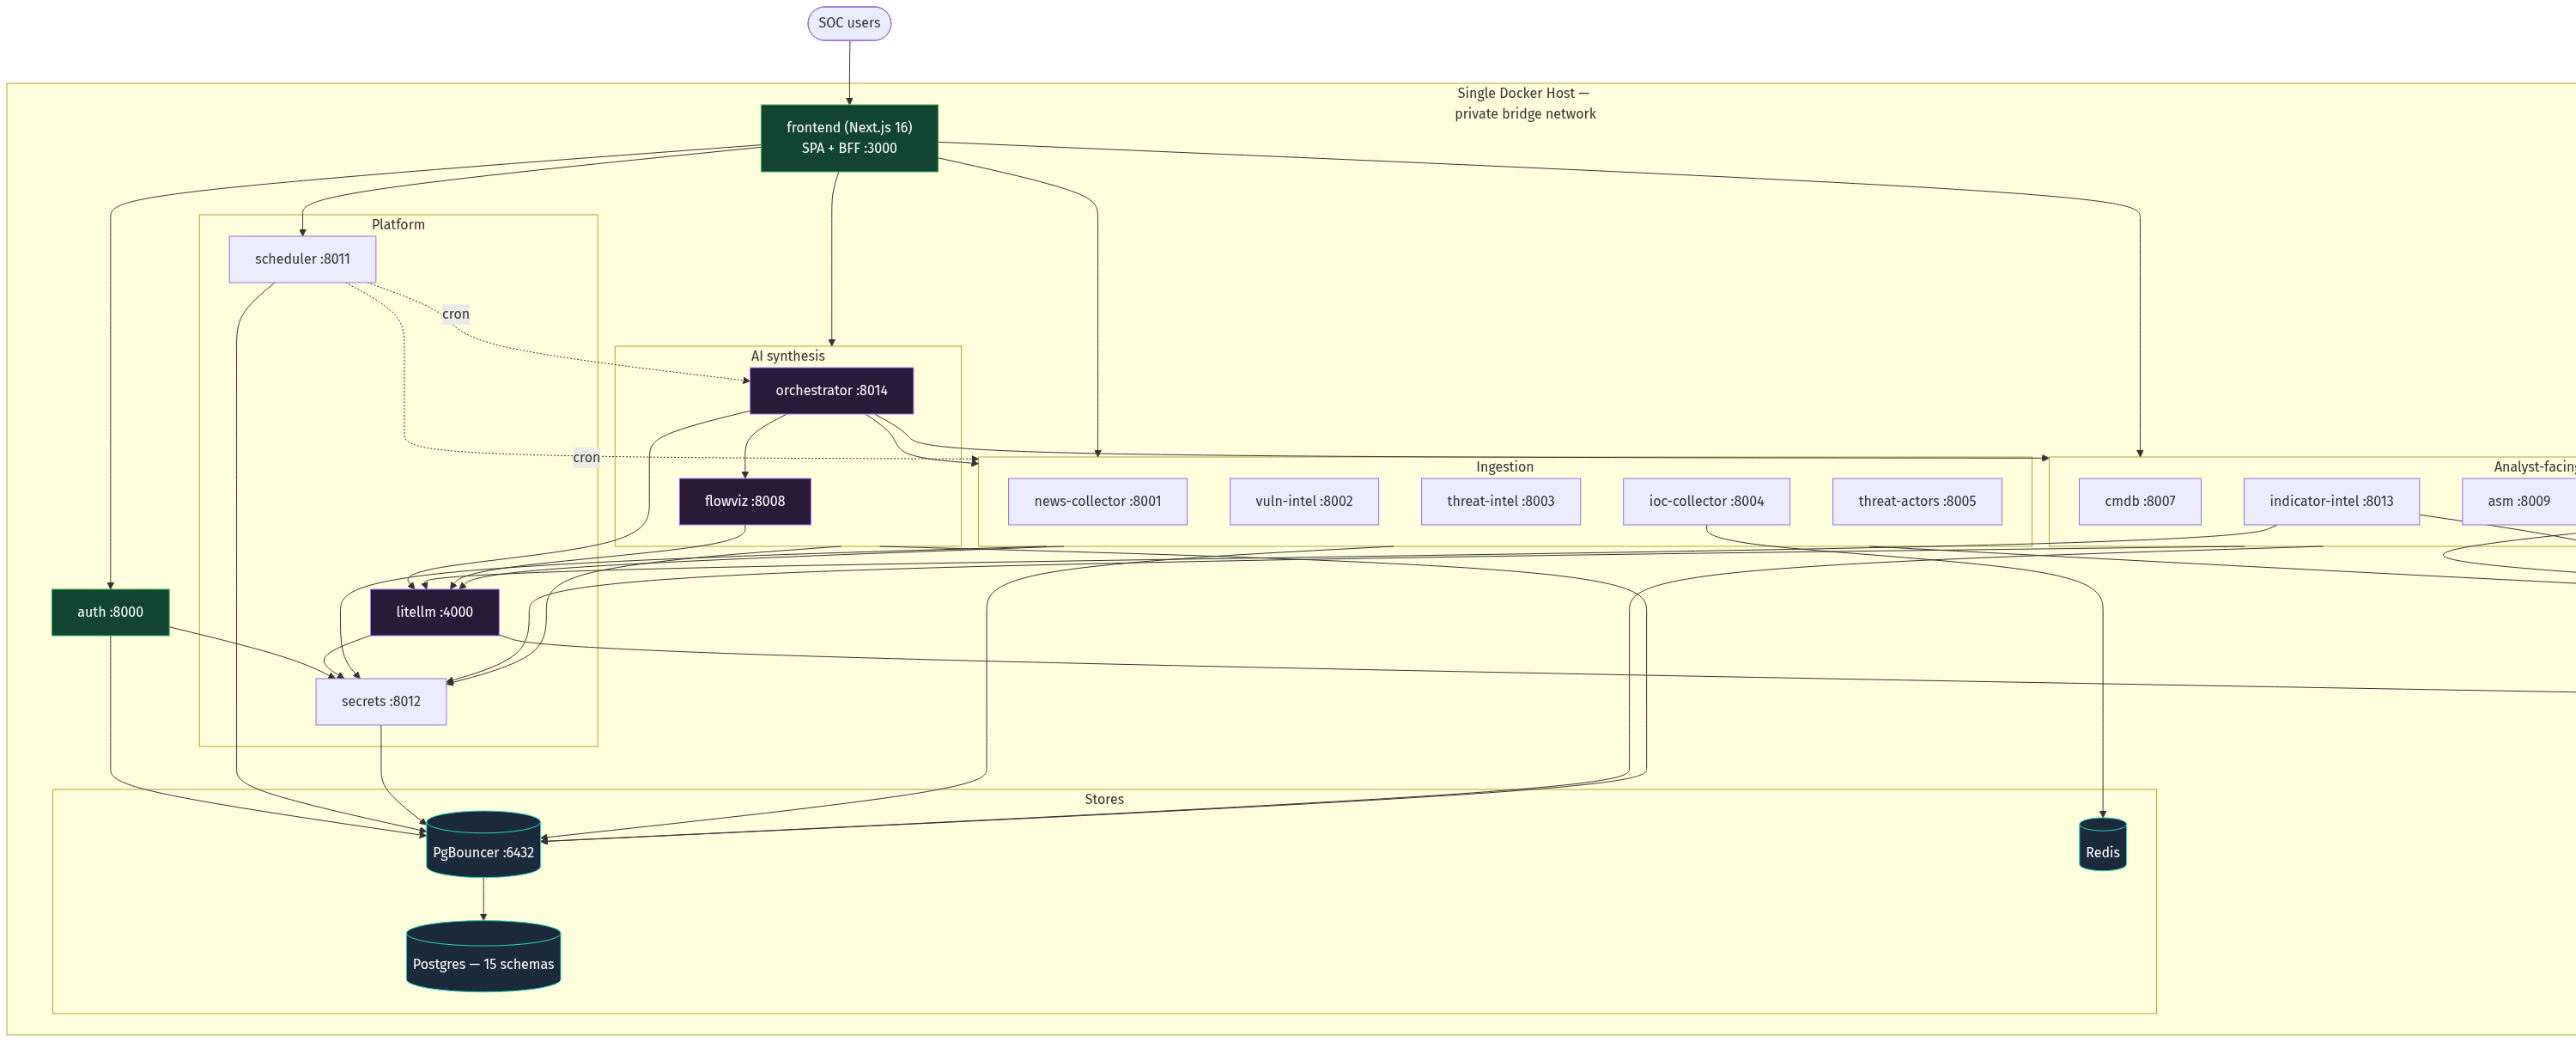
\includegraphics[width=\textwidth]{images/tip/diagrams/05_global_architecture_core.png}
\caption{Global system architecture, core platform topology.}
\label{fig:global-arch}
\end{figure}

\begin{figure}[H]
\centering
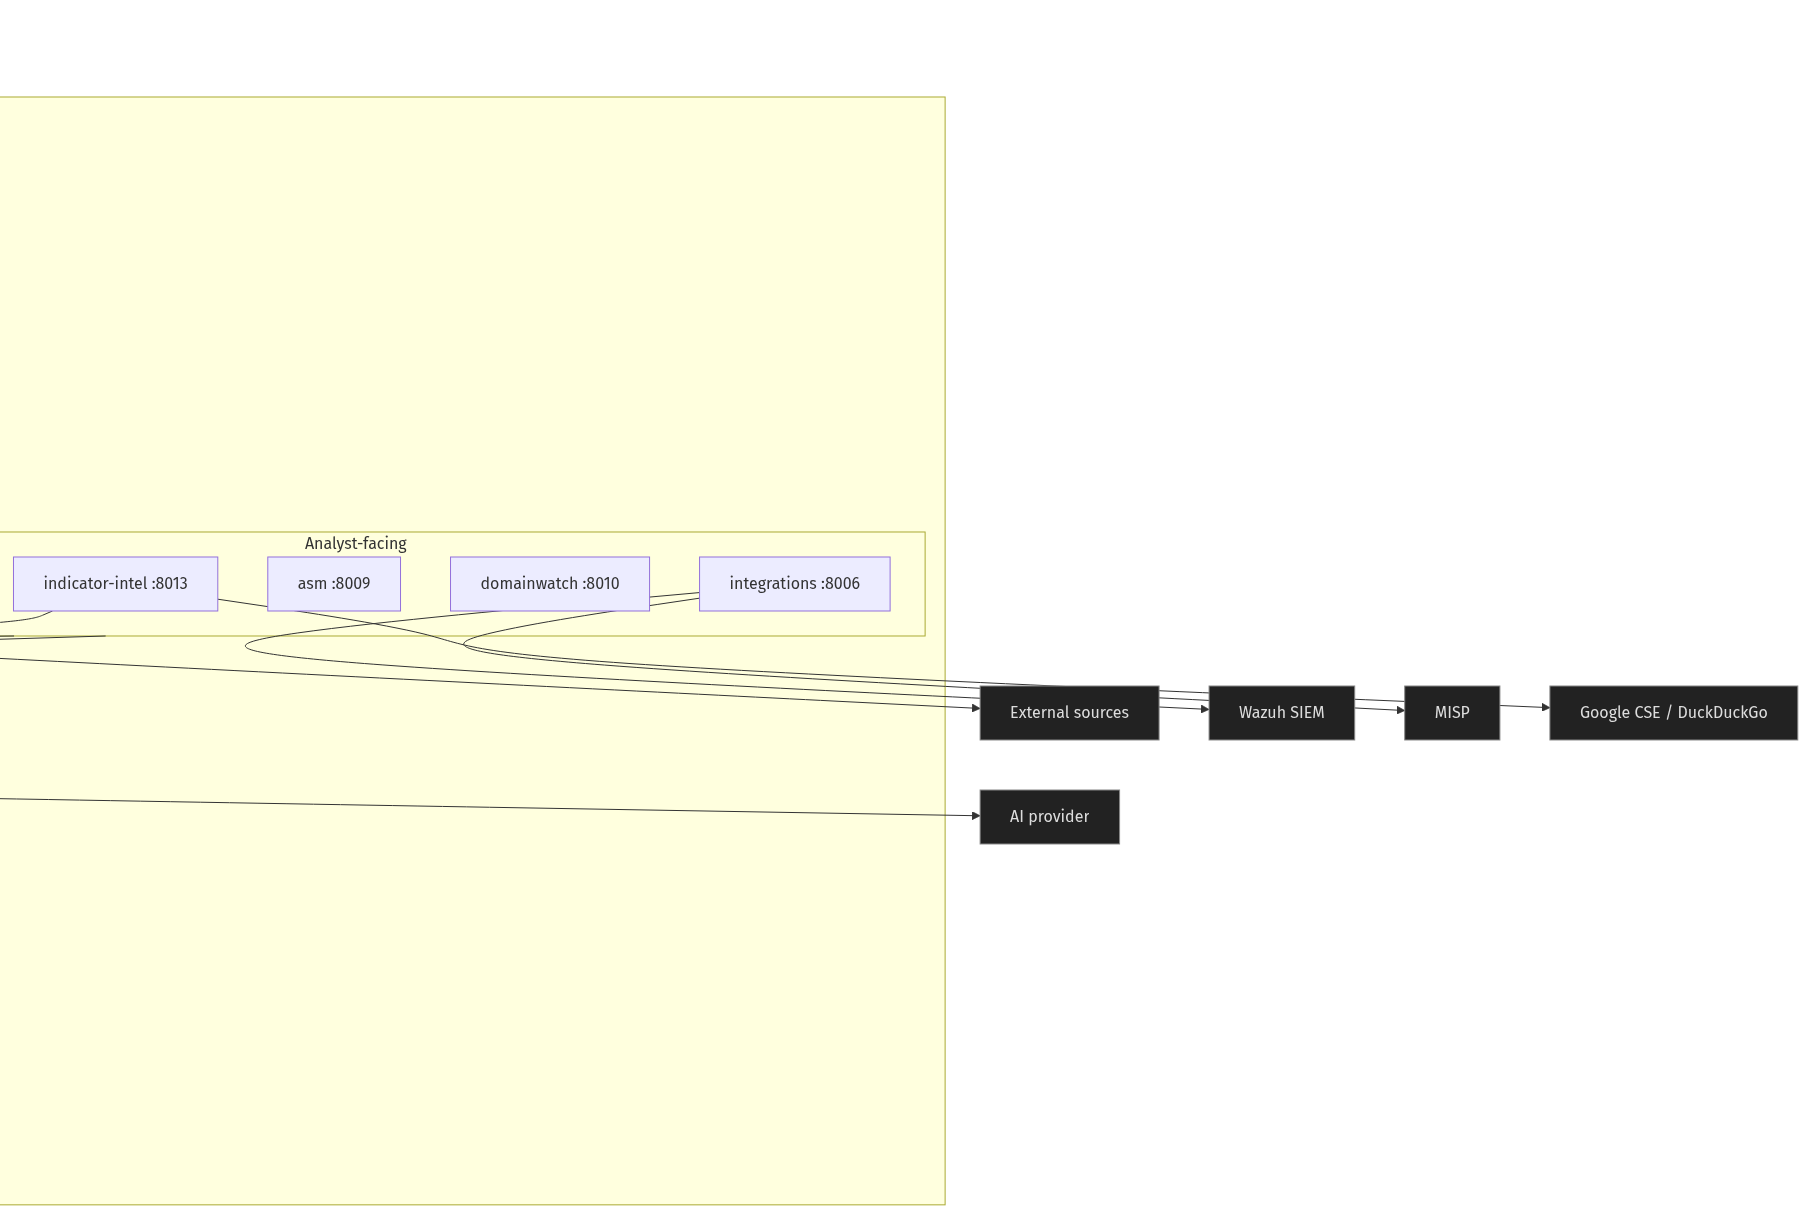
\includegraphics[width=0.92\textwidth]{images/tip/diagrams/05_global_architecture_integrations.png}
\caption{Global system architecture, analyst-facing edge and external integrations.}
\label{fig:global-arch-ext}
\end{figure}

\begin{table}[H]
\centering
\caption{Service catalogue and primary responsibility}
\label{tab:service-catalogue-new}
\renewcommand{\arraystretch}{1.2}
\begin{tabular}{|p{3.2cm}|p{2.2cm}|p{1.5cm}|p{6.0cm}|}
\hline
\textbf{Service} & \textbf{Layer} & \textbf{Port} & \textbf{Primary responsibility}\\
\hline
auth & platform & 8000 & user login, refresh tokens, RBAC, service identity\\
\hline
news-collector & ingestion & 8001 & article feed ingestion and article views\\
\hline
vuln-intel & ingestion & 8002 & CVE, EPSS, KEV refresh and vulnerability views\\
\hline
threat-intel & ingestion & 8003 & public threat reporting, supply-chain and breach context\\
\hline
ioc-collector & ingestion & 8004 & indicator ingestion, normalization, lookup\\
\hline
threat-actors & ingestion & 8005 & actor, ransomware, TTP and tool intelligence\\
\hline
integrations & analyst & 8006 & Wazuh and MISP integration surfaces\\
\hline
cmdb & analyst & 8007 & assets, tags, company profile, organizational context\\
\hline
flowviz & synthesis & 8008 & attack-flow generation and rendering support\\
\hline
asm & analyst & 8009 & passive attack-surface discovery workflows\\
\hline
domainwatch & analyst & 8010 & domain monitoring and screenshot capture\\
\hline
scheduler & platform & 8011 & recurring jobs and run-history management\\
\hline
secrets & platform & 8012 & encrypted secret storage and bootstrap fetch\\
\hline
indicator-intel & analyst & 8013 & deep indicator investigation and dorking workflows\\
\hline
orchestrator & synthesis & 8014 & AI synthesis, reporting, Q\&A, policies, actions\\
\hline
\end{tabular}
\end{table}

\section{Architectural Decomposition}
\subsection{Ingestion Services}
The ingestion layer is responsible for obtaining intelligence from external providers, transforming it into a stable internal shape, and storing it durably. Each service owns one intelligence domain, which limits failure blast radius and keeps external-source logic localized. News, vulnerabilities, indicators, actors, and threat reporting are therefore refreshed independently and can degrade independently.

\subsection{Analyst-Facing Services}
The analyst layer exposes the context required to interpret intelligence operationally. CMDB represents assets and the organization profile. Integrations exposes operational telemetry from Wazuh and MISP. ASM and domainwatch provide exposure-oriented views that complement pure threat feeds. Indicator-intel performs slower, investigation-grade enrichment when a quick IOC verdict is insufficient.

\subsection{Synthesis Services}
The synthesis layer is centred on the orchestrator. It does not ingest raw feeds directly. Instead, it fans out over the other services' HTTP interfaces, assembles context, executes structured AI analysis, and persists outputs such as reports, rankings, and correlations. Flowviz complements this by generating graphable attack-flow structures from textual or analytical inputs.

\subsection{Platform Services}
The platform layer contains the shared control-plane functions: authentication, secret management, scheduling, and AI gatewaying. Centralizing these concerns reduces duplication and keeps high-sensitivity logic in a small number of services.

This four-layer decomposition also reflects a theoretical distinction between data acquisition, context exposure, analytical transformation, and platform governance. The ingestion layer acquires and shapes knowledge. The analyst layer exposes organization-specific context and operational surfaces. The synthesis layer performs cross-domain reasoning. The platform layer governs trust, configuration, and execution. This separation is useful academically because it explains why similarly technical components belong to different layers: the criterion is not implementation language or container image, but role in the knowledge-production process.

\section{Backend Architecture and Shared Service Shape}
All backend services share one construction pattern. The shared factory in \texttt{tip\_common} configures structured logging, correlation-ID middleware, error handlers, and a health endpoint. Startup hooks then initialize per-service state such as database engines, cache clients, secret clients, source-health repositories, AI clients, and scheduler instances. Auth middleware is intentionally not added in the shared factory because services often need to fetch the verification key during startup before requests can be validated.

This pattern is important architecturally because it delivers two forms of consistency at once. Services remain thin and domain-focused, but operational concerns such as logging, correlation, error translation, and settings handling are solved once in the shared layer. Figure~\ref{fig:module-deps} shows the dependency direction between services and shared libraries.

From a software-engineering perspective, this is a deliberate use of an internal platform layer. Instead of expecting each service to rediscover how to log, manage settings, expose health, handle correlation IDs, or map exceptions, the shared packages encode those concerns once and make them cheap to reuse. The result is a service portfolio with lower accidental variation. This matters because in multi-service systems, ungoverned local variation often becomes a larger source of operational fragility than the domain logic itself.

\begin{figure}[H]
\centering
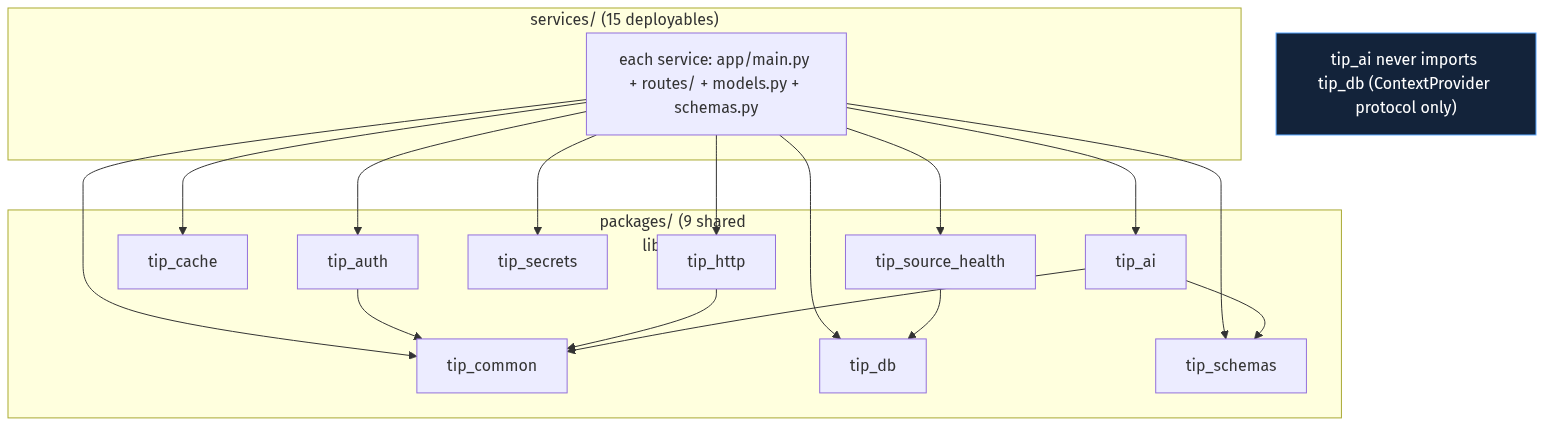
\includegraphics[width=0.92\textwidth]{images/tip/diagrams/14_module_dependencies.png}
\caption{Dependency direction between shared packages and services.}
\label{fig:module-deps}
\end{figure}

\section{Frontend Architecture and the BFF Pattern}
The frontend is a Next.js application using the App Router. Its role is more significant than a simple presentation layer. It serves as the browser-facing entry point and hosts the backend-for-frontend proxy under \texttt{/api/*}. The catch-all BFF route maps path prefixes to backend services and forwards headers, query parameters, and request bodies accordingly.

This design provides three concrete benefits. First, it gives the browser one consistent origin and one consistent API surface. Second, it keeps backend service URLs and routing logic centralized in one place. Third, it allows the frontend to expose aggregate routes such as the dashboard endpoint, which fans out to multiple services in parallel and returns a single response tailored to the user interface.

The frontend stores user state and permissions in a persisted client-side store and uses that state to attach Bearer tokens to BFF requests. This must be stated precisely because it differs from a stricter cookie-only edge model. The current deployment relies on client-held tokens plus a BFF proxy, not on HTTP-only cookie injection.

Theoretically, the BFF layer resolves a representational mismatch. Backend services are designed around domain ownership, not around page composition. A dashboard, for example, is not a natural object in the vulnerability or actor services by themselves. It is a frontend concern that requires aggregated, latency-aware composition. The BFF therefore improves not only security posture but also interface ergonomics. It allows the user interface to evolve without forcing every backend service to become UI-aware.

\section{Request and Communication Patterns}
The platform is deliberately message-light. The dominant coordination mechanism is HTTP, both from browser to BFF and between internal services. Figure~\ref{fig:req-flow} illustrates the main request lifecycle.

\begin{figure}[H]
\centering
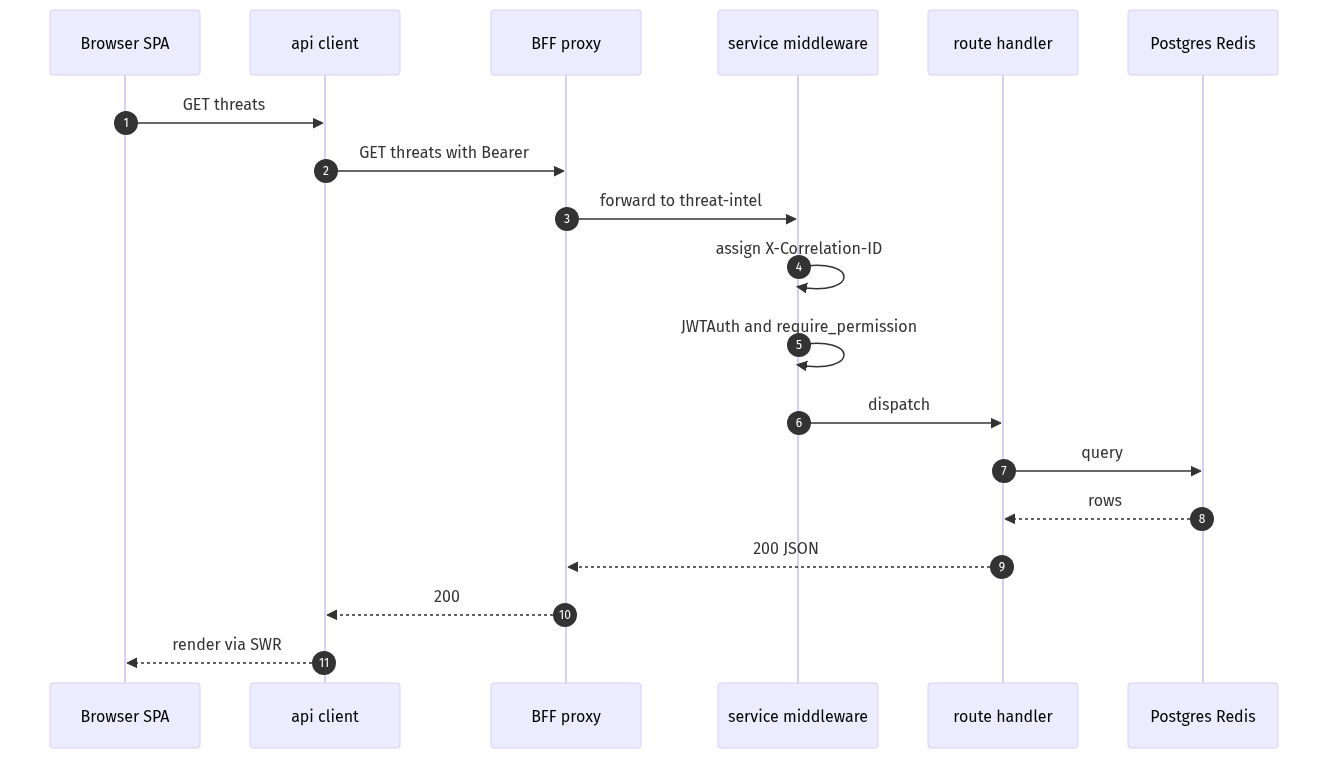
\includegraphics[width=0.92\textwidth]{images/tip/diagrams/05_request_flow.png}
\caption{Request flow from frontend to backend services.}
\label{fig:req-flow}
\end{figure}

Four recurring communication patterns appear across the system.

\subsection{Synchronous Read Paths}
Most read endpoints return stored data directly from Postgres, optionally mediated by Redis for hot lookups. This keeps user-visible latency bounded by local infrastructure rather than external feeds.

\subsection{Scheduler-Triggered Control Paths}
Recurring work is initiated by the scheduler through HTTP POST calls that carry a generated run identifier. Endpoints may complete synchronously or accept work and complete it asynchronously via callback. This pattern preserves a simple control plane while still supporting long-running jobs.

\subsection{Context Fan-Out}
The orchestrator performs multi-leg fan-out calls to assemble the context needed for synthesis. It does not bypass service boundaries by reading their tables directly. This is one of the strongest indicators that the service decomposition is real rather than nominal.

\subsection{Bootstrap and Secret Retrieval}
Services use a pre-authentication bootstrap path to obtain secrets needed before they have a JWT. The same pattern is used to obtain the auth public key and service bootstrap tokens during startup.

Figure~\ref{fig:service-interactions} summarizes the most important inter-service interactions.

\begin{figure}[H]
\centering
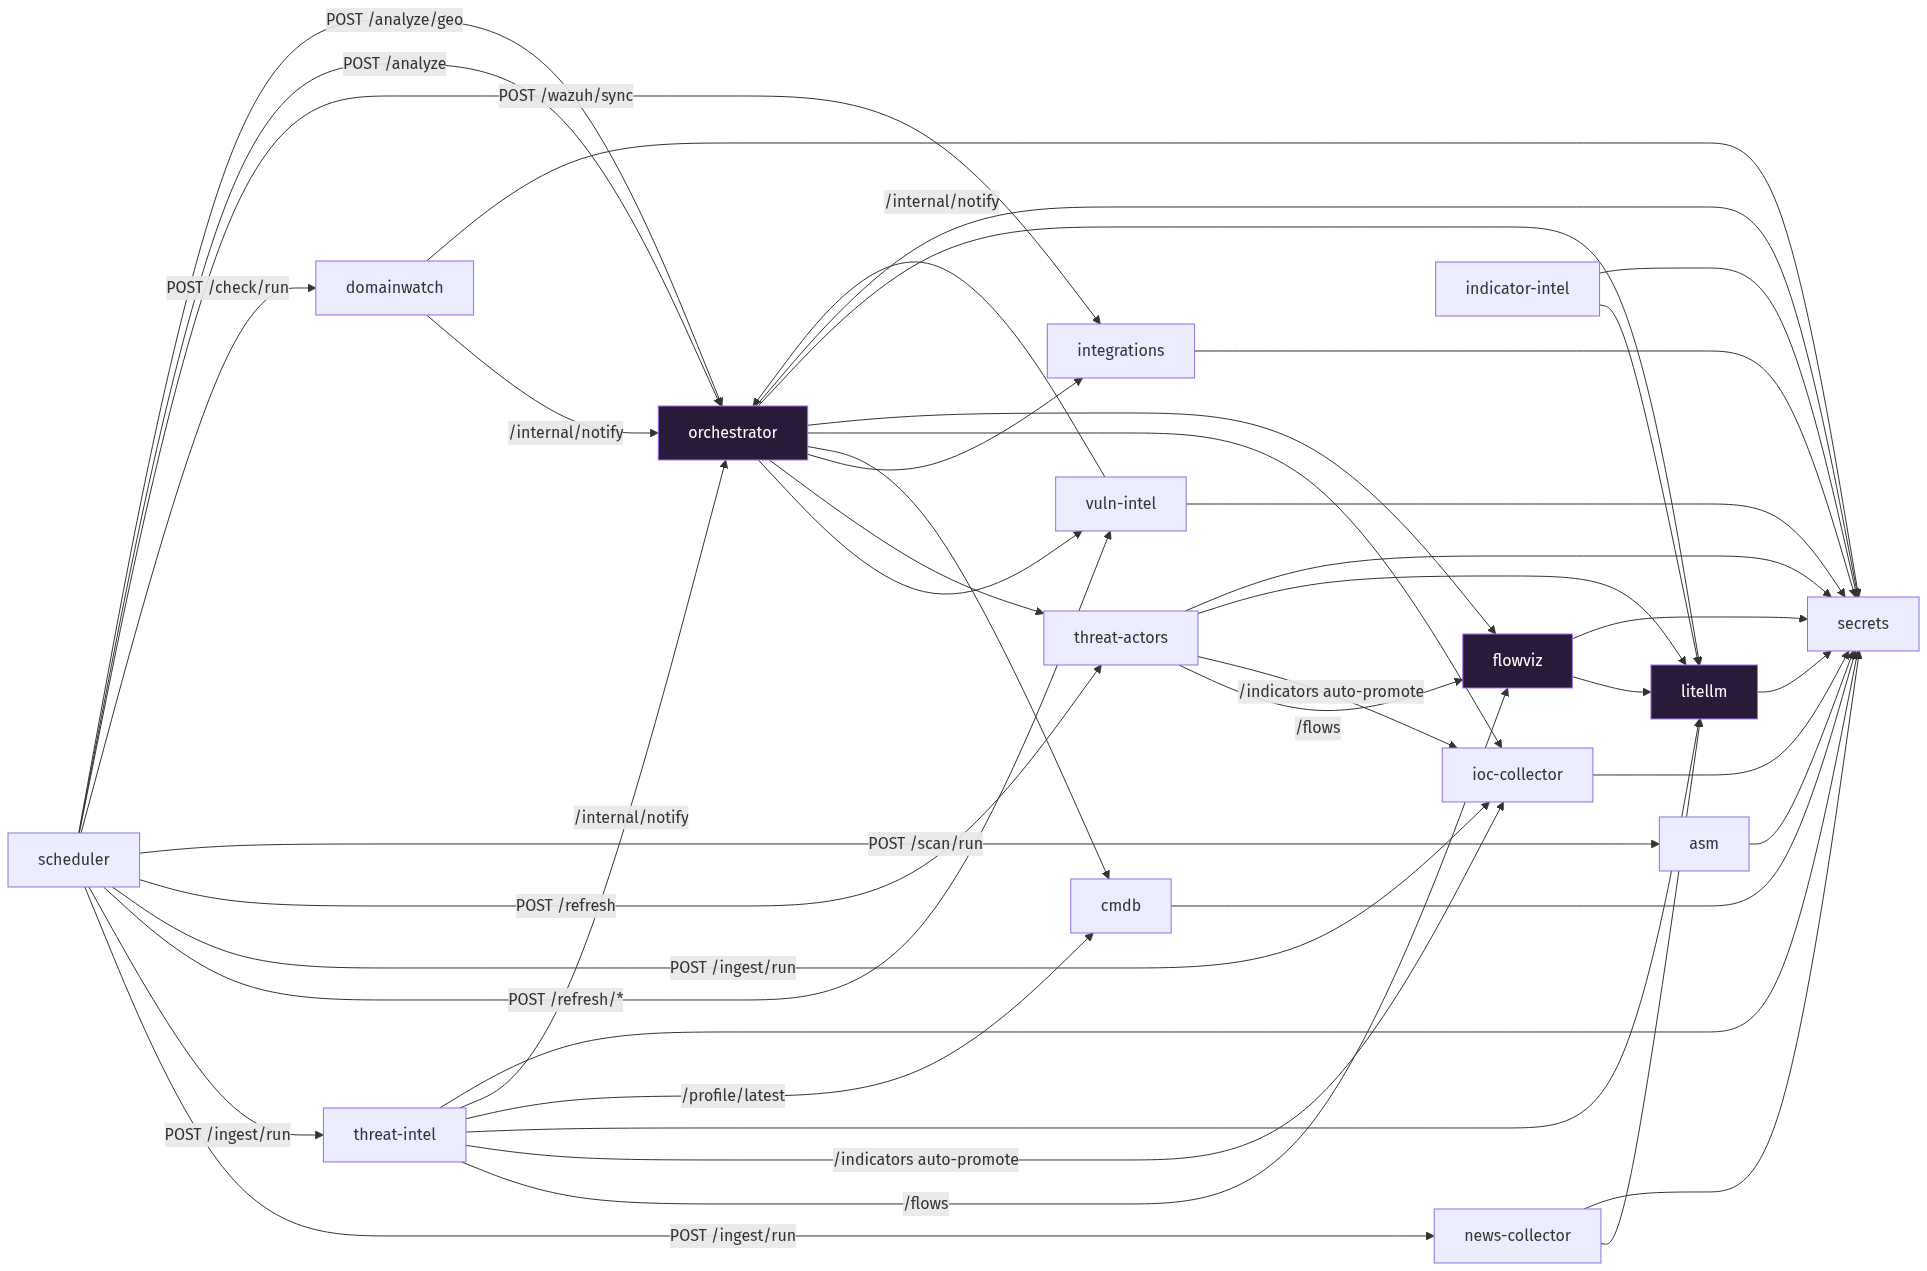
\includegraphics[width=0.95\textwidth]{images/tip/diagrams/05_service_interactions.png}
\caption{Primary inter-service interactions.}
\label{fig:service-interactions}
\end{figure}

\section{Data Architecture}
\subsection{One Database, Many Schemas}
All services share one PostgreSQL database, but logical isolation is maintained by schema partitioning. Each service owns its own schema, migrations, and ORM models. No foreign key crosses a schema boundary. Cross-service relations are resolved through stable identifiers and HTTP APIs rather than joins across tables.

This design is a compromise between operational simplicity and service isolation. A database-per-service model would have increased operational cost significantly for the target deployment. A single shared schema would have undermined modularity. The chosen approach preserves one backup domain and one database process while still allowing per-service ownership.

The database architecture is therefore best understood as a layered compromise. It accepts a shared physical store while preserving logical ownership boundaries. This avoids a common false binary in service-oriented design: either every service gets its own full infrastructure stack, or all services collapse into one undifferentiated data model. The chosen solution preserves the migration path toward stronger physical separation later without paying the operational cost upfront.

\begin{figure}[H]
\centering
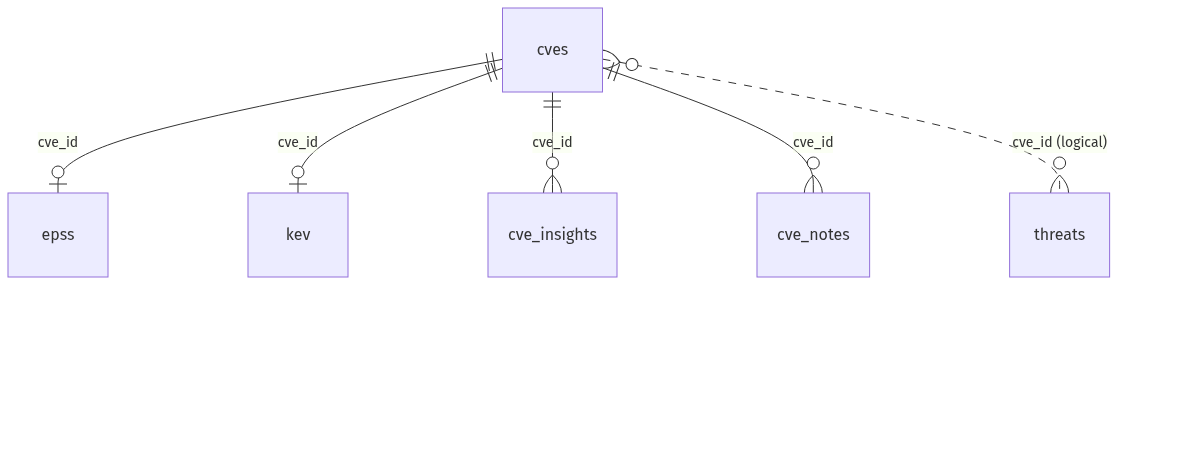
\includegraphics[width=\textwidth]{images/tip/diagrams/07_erd_left.png}
\caption{High-level entity relationship structure across service schemas, part 1.}
\label{fig:erd-new}
\end{figure}

\begin{figure}[H]
\centering
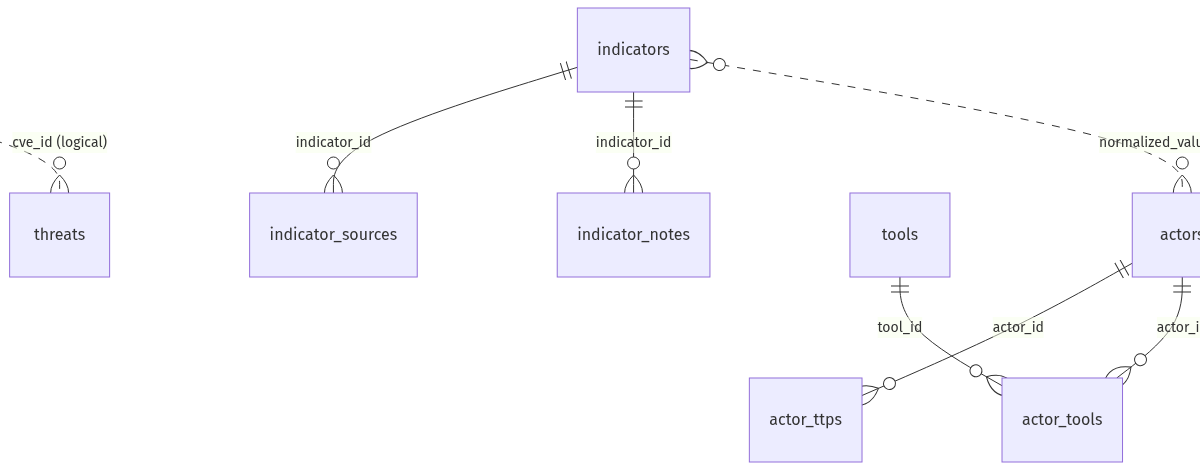
\includegraphics[width=\textwidth]{images/tip/diagrams/07_erd_center.png}
\caption{High-level entity relationship structure across service schemas, part 2.}
\end{figure}

\begin{figure}[H]
\centering
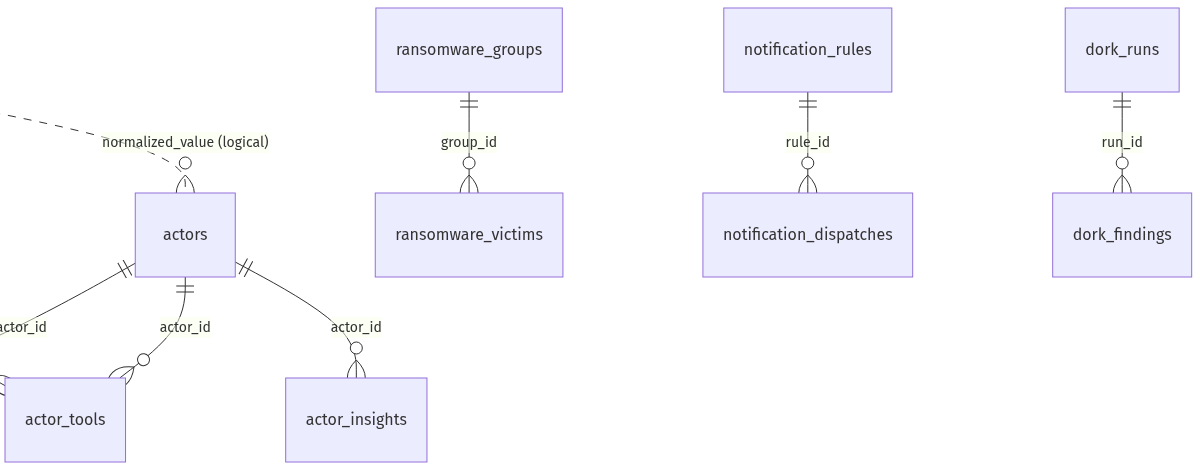
\includegraphics[width=\textwidth]{images/tip/diagrams/07_erd_right.png}
\caption{High-level entity relationship structure across service schemas, part 3.}
\end{figure}

\subsection{PgBouncer and Pooler-Aware Access}
PgBouncer sits between application services and Postgres in transaction-pooling mode. This is not a cosmetic optimisation. It allows fifteen services to share a bounded set of backend connections without exhausting the database. It also imposes constraints on the SQLAlchemy configuration: prepared-statement caching is disabled and connections are pre-pinged and recycled to tolerate pooler behaviour and stale backends.

\begin{figure}[H]
\centering
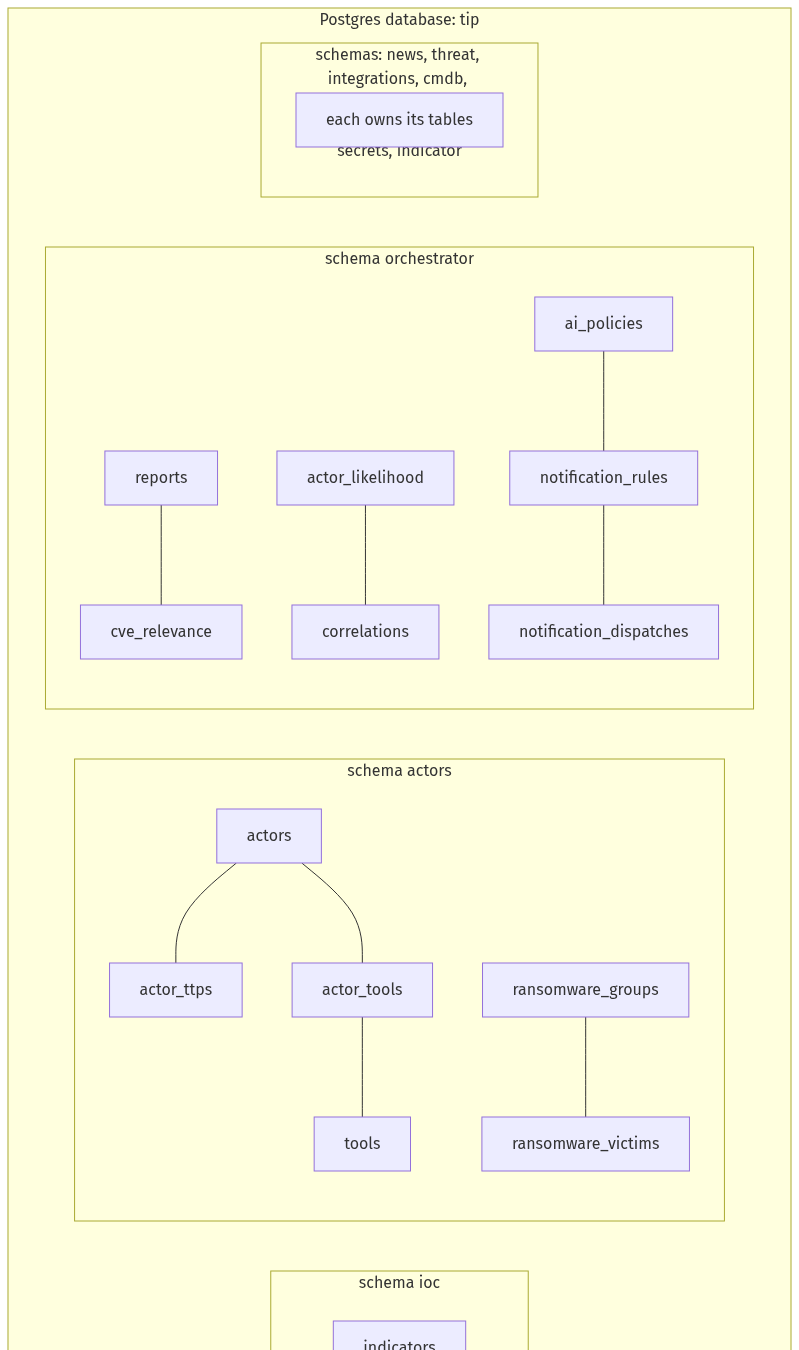
\includegraphics[width=0.74\textwidth]{images/tip/diagrams/07_relational_model_top.png}
\caption{Relational topology with PgBouncer between services and PostgreSQL, upper segment.}
\label{fig:relational-model-new}
\end{figure}

\begin{figure}[H]
\centering
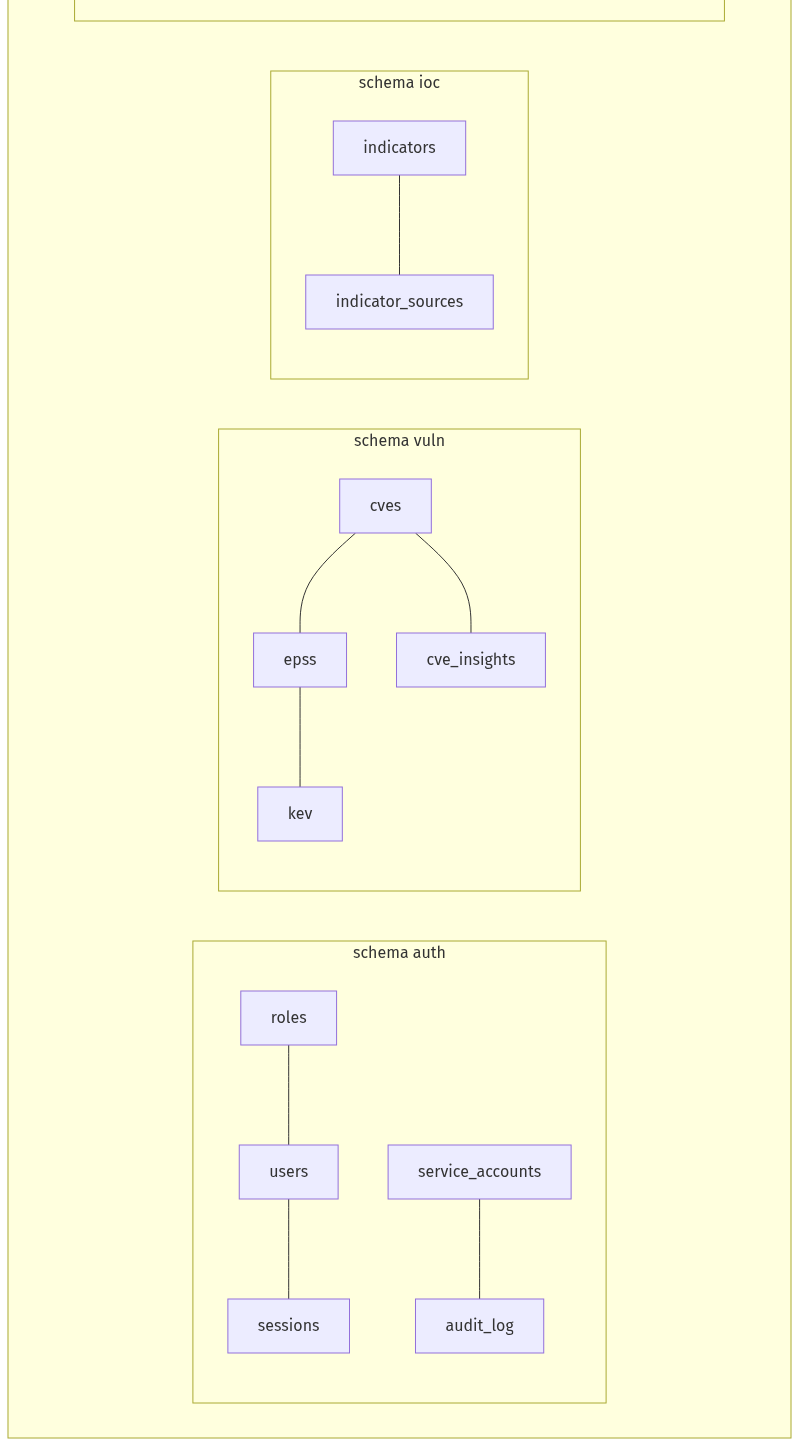
\includegraphics[width=0.74\textwidth]{images/tip/diagrams/07_relational_model_bottom.png}
\caption{Relational topology with PgBouncer between services and PostgreSQL, lower segment.}
\end{figure}

\subsection{JSON for Fidelity, Relational Columns for Queries}
Many records retain upstream payloads in JSON form while also extracting searchable relational fields. This is an important engineering choice. The relational columns support fast query patterns, sorting, and filtering. The JSON payloads preserve source fidelity and support reprocessing without having to fetch historical data again.

This hybrid storage model addresses a common tension in intelligence systems. Purely relational schemas are excellent for structured query and constraint enforcement, but they can be too rigid for heterogeneous and evolving source payloads. Pure document storage preserves source richness but can make common analytical queries and joins inefficient or ambiguous. By combining relational projections with retained upstream JSON, the platform preserves both operational queryability and evidentiary fidelity.

\section{Authentication, Authorization, and Trust Boundaries}
\subsection{Actual Trust Model}
The trust model must be described carefully. The auth service validates user credentials, issues RS256 access tokens and refresh tokens, and exposes role and session administration. However, in the current Docker Compose deployment, most non-auth services inherit \texttt{DISABLE\_AUTH=true} on the private Docker network, while auth itself runs with enforcement enabled. In practice, this means the platform's strongest trust boundary is between the browser-facing layer and the internal service network, not between every pair of internal services.

This is a deliberate simplification, not an implementation accident. It reduces failure modes associated with service-to-service token validation, but it also weakens internal segmentation. Any academic treatment of the platform must present both sides of that tradeoff.

\subsection{RBAC Enforcement}
Where auth is enforced, permissions are checked through a single shared dependency, \texttt{require\_permission}. This keeps authorization logic declarative at route level and makes permission intent visible in code. The auth service's \texttt{/me} route rehydrates the current user state from the database instead of trusting stale JWT claims, which is a stronger pattern than naive claim-only identity handling.

\subsection{Secrets Management}
All secrets except the Fernet key and the shared bootstrap token are stored in the secrets service, encrypted at rest. Services fetch required secrets during startup. Access to secrets is audited. The LiteLLM proxy retrieves provider API keys from the vault at startup, which means downstream analytical services generally hold only the proxy master key rather than direct provider credentials.

From a design-theory perspective, the trust model is intentionally asymmetric. User-originated traffic is handled with much stronger authentication expectations than internal service-to-service traffic in the current deployment profile. This is not the purest possible design, but it is legible and defensible if described honestly. It reduces some operational coupling while preserving a clear future hardening path toward stronger internal verification.

\section{Security Boundary and External Exposure}
The deployment aims to minimize external exposure, but the reality must be stated accurately. The frontend is the intended browser-facing application. However, the compose file also publishes several backend ports for direct access and diagnostics. The architecture should therefore be described as a deployment with a primary edge at the frontend plus additional exposed service ports, not as a perfectly single-port system.

This distinction matters because it affects how the security chapter should reason about hardening, monitoring, and future improvements.

\section{Caching and Source Health as Architectural Components}
Redis is used as a loss-tolerant accelerator rather than as a system of record. Hot-path indicator results, transient AI responses, and source-health state are cached with bounded TTLs. The durable source of truth remains PostgreSQL. The source-health subsystem spans cache and database: Redis provides fast checks for open circuits, while the per-service source-health tables provide durable operator visibility.

This is architecturally important because cache and health state are not treated as incidental implementation details. They are part of the system's control logic. Source health influences whether the platform should continue attempting upstream calls. Cache state influences whether the platform can respond at operational speed. In that sense, both are first-class architectural elements rather than mere optimizations.

\section*{Conclusion}
\addcontentsline{toc}{section}{Conclusion}
The delivered architecture is a modular, HTTP-coordinated, single-host security platform shaped more by operational clarity than by distributed-systems maximalism. Its strongest properties are consistent service construction, clear domain boundaries, schema ownership, explicit control-plane services, and a practical BFF layer. Its most important caveat is that the internal trust model is simpler and more permissive than a strict service-mesh security story would suggest. The next chapter explains the platform technologies and infrastructure stack that make this architecture operationally viable, before the report turns to the service catalogue and implementation mechanics.

\chapter{Infrastructure and Platform Technologies}
\thispagestyle{plain}
\section*{Introduction}
\addcontentsline{toc}{section}{Introduction}
A reader who is not already fluent in modern web and distributed-platform tooling cannot be expected to infer the role of each technology from a deployment diagram alone. This chapter therefore explains the main infrastructural and framework choices used by the platform, the theory behind them, and the specific problem each one solves in this project. The goal is not to catalogue fashionable tools. The goal is to show why each technology exists in the architecture and what engineering pressure it relieves.

\section{Containerization and Environment Reproducibility}
\subsection{What Docker Is}
Docker is a containerization platform that packages an application together with its runtime dependencies, entrypoint, filesystem layers, and environment assumptions into an isolated unit that can be started consistently across machines \cite{docker_docs}. A container is lighter than a full virtual machine because it shares the host kernel, but it still provides process-level and filesystem-level isolation relative to other applications.

\subsection{What Problem Docker Solves in This Project}
The platform contains fifteen backend services, a frontend, a database, a connection pooler, a cache, a LiteLLM gateway, and bootstrap containers. Without containerization, reproducing the runtime environment would require manually installing Python versions, Node tooling, system packages, database services, Redis, browser dependencies for screenshot capture, and correct environment variables on every target host. That approach is fragile and makes deployment drift likely.

In this project, Docker solves three problems simultaneously. First, it makes the build and execution environment reproducible. Second, it isolates service-specific dependencies, which is important because not every service needs the same Python packages or system libraries. Third, it enables the platform to be brought up and torn down predictably as one application stack rather than as a sequence of manual operations.

\subsection{Why Containerization Is Theoretically Appropriate Here}
Containerization is especially suitable when services are largely stateless at process level but depend on externalized state such as databases, caches, and volumes. That is the case for this platform. The services can be rebuilt and restarted independently, while PostgreSQL, Redis, and persistent mounted storage preserve the durable state. This creates a clear separation between application process lifecycle and data lifecycle.

\subsection{Images, Layers, and Immutability}
One of Docker's most important theoretical ideas is immutability of runtime artefacts. A container image is built from filesystem layers. Once built and versioned, that image becomes a reproducible description of the runtime environment. This reduces the risk of configuration drift because deployment changes are expressed as new images rather than as undocumented manual edits on the host.

In this project, that property is particularly valuable because the platform includes heterogeneous services with different runtime needs. Some services need browser-capable environments, others need only Python and HTTP clients, and the frontend needs a Node-based toolchain. Layered images allow each service to carry exactly the dependencies it requires while remaining reproducible.

\subsection{Networks and Volumes}
Docker also provides two abstractions that are especially relevant here: virtual networks and named volumes. Networks create controlled service-to-service communication domains. Volumes preserve state independently of container lifecycle. In the platform, networks express the private service fabric, while volumes preserve data such as PostgreSQL state, Grafana state where applicable, and generated artefacts.

The theoretical value of these abstractions is that they separate communication topology and durable state from process identity. A service can be recreated without redefining either its network placement or its persisted data.

\subsection{Isolation Boundaries and Their Limits}
It is also important to explain what containers do \emph{not} solve. Docker provides process isolation, namespace separation, packaging control, and a cleaner operational boundary than unmanaged host processes. It does not provide the same isolation assumptions as a full hypervisor. Containers still share the host kernel. From a security-theory standpoint, that means containerization improves deployment hygiene and boundary clarity, but it should not be mistaken for a complete trust-separation mechanism.

This distinction matters in the project because the platform is deployed on one host with many cooperating services. The security benefit of Docker here is mainly reproducibility, scoped runtime composition, and reduced dependency sprawl. Stronger hostile-tenant isolation is not the primary deployment goal.

\section{Docker Compose and Single-Host Orchestration}
\subsection{What Docker Compose Is}
Docker Compose is a declarative orchestration tool for defining multi-container applications: images, environment variables, networks, health checks, startup dependencies, volumes, and published ports can be described in one file \cite{docker_compose_docs}. It is not a cluster orchestrator like Kubernetes. Its strength is controlled, comprehensible single-host composition.

\subsection{What Problem Compose Solves in This Project}
The project is explicitly targeted at a small team and a single-host deployment model. That means the relevant problem is not dynamic cluster scaling. It is reliable local orchestration. Compose solves the problem of coordinating many dependent services with one command surface. It ensures the same network topology, dependency ordering, environment wiring, and volume mapping are reproduced each time the stack is started.

\subsection{Why Kubernetes Was Not the Right Default Choice}
From a theoretical perspective, orchestration should match operational scale. Kubernetes would provide stronger scheduling and scaling abstractions, but it would also introduce higher operational complexity, more control-plane components, and a steeper learning burden for a team whose primary problem is intelligence workflow integration, not cluster management. Compose is therefore not a lesser version of a ``real'' architecture here; it is the architecture that best fits the actual deployment constraint.

\subsection{Declarative Infrastructure and Day-Two Operations}
Compose also has methodological value because it is declarative. The topology, health dependencies, environment wiring, volumes, and ports are written down in a machine-readable form. This matters for day-two operations because the running system can be recreated from the same description rather than from operator memory. In other words, Compose is not only a launch tool; it is part of the platform's executable documentation.

\subsection{Dependency Ordering, Health Checks, and Controlled Startup}
Single-host orchestration still has a sequencing problem. Databases must be reachable before dependent services can acquire sessions correctly. Secrets must be available before services that need bootstrap material can complete startup. Frontend routes should not become user-facing before the underlying application surfaces are minimally functional. Compose addresses part of this through dependency and health-check declarations.

The broader theoretical point is that system correctness is not only about steady-state behaviour. It is also about transitional states such as startup, restart, and recovery. A platform that behaves correctly only after manual babysitting is architecturally weaker than one whose startup dependencies are expressed directly in its orchestration layer.

\section{PostgreSQL as the System of Record}
\subsection{What PostgreSQL Is}
PostgreSQL is a relational database system with strong transactional guarantees, rich indexing, JSON support, and mature ecosystem tooling \cite{postgresql_docs}. It is appropriate when data must be queried flexibly, updated safely, and retained durably.

\subsection{What Problem PostgreSQL Solves in This Project}
The platform ingests many entity types: CVEs, EPSS entries, KEV flags, indicators, actor records, reports, sessions, notes, rules, notifications, and more. These entities are not isolated lists. They must be filtered, sorted, joined conceptually, enriched, versioned, and queried through API endpoints. PostgreSQL provides the durable store for this knowledge and allows the system to answer operational queries reliably.

\subsection{Why a Relational Store Is Appropriate}
A purely document-oriented store would preserve source payloads easily but make many cross-entity and filter-driven queries less disciplined. A graph database would model some CTI relationships elegantly but would add operational complexity and still not remove the need for transactional application data. PostgreSQL represents a practical middle ground: relational enough for operational queries and constraints, yet flexible enough through JSON columns to preserve heterogeneous upstream payloads.

\subsection{ACID, Transactions, and Why They Matter Here}
Relational databases remain especially strong when applications need transactional integrity. The classical ACID properties, atomicity, consistency, isolation, and durability, are not abstract textbook ideas in this platform. They matter because updates often affect logically related state: sessions must be created and revoked safely, scheduled job state must transition coherently, and ingest operations must either persist valid records or fail without leaving ambiguous partial state.

Atomicity ensures that a multi-step write is not partially committed in a way that corrupts workflow state. Consistency ensures schema and application constraints continue to hold. Isolation matters when many services operate concurrently over shared infrastructure. Durability ensures that once a record is committed, it persists beyond process failure. These properties are one reason a relational database is so appropriate for the platform's control-plane and knowledge-store responsibilities.

\subsection{MVCC and Concurrent Reads}
PostgreSQL's multi-version concurrency control (MVCC) is also relevant conceptually. MVCC allows readers and writers to coexist with less blocking than simpler locking models. In a platform with many services, read-heavy APIs, and periodic ingest or synthesis writes, this matters because the system cannot afford for common reads to become excessively blocked by ordinary update activity. MVCC is therefore part of the reason PostgreSQL scales acceptably for this mixed read/write intelligence workload.

\subsection{Indexing, Queryability, and Operational Search}
Threat-intelligence data is only useful if it can be searched and filtered quickly. A database in this kind of system is not just archival storage. It is a live query engine. PostgreSQL's indexing capabilities, combined with relational projections of key fields, make it suitable for list views, filtered dashboards, IOC lookups, CVE retrieval, and session or rule management. This is another reason the platform favours structured relational storage for query-relevant fields while preserving upstream JSON for completeness.

\subsection{Constraints as Data-Governance Mechanisms}
Database constraints also deserve explicit attention. Primary keys, foreign keys, unique constraints, and check constraints are not mere implementation details. They are governance mechanisms that prevent invalid system states from becoming durable. In a CTI platform this matters because normalization errors, duplicate identities, malformed relationships, or orphaned records can quietly poison downstream analysis.

At the thesis level, this is one of the reasons relational persistence remains attractive. The database can actively participate in preserving semantic hygiene rather than acting as a passive bag of bytes.

\section{Schema Partitioning and Logical Multi-Tenancy by Service}
The platform keeps one PostgreSQL instance but partitions ownership by schema. This means each service owns its own tables, migrations, and model evolution while still sharing one physical database process. The theory behind this choice is service isolation without unnecessary infrastructure multiplication. It preserves data ownership boundaries, reduces accidental coupling, and still fits the single-host operational model.

Schema partitioning is also useful pedagogically because it exposes service ownership clearly. If every service wrote into one undifferentiated schema, it would become harder to distinguish domain boundaries, migration responsibility, and accidental data coupling. By retaining one schema per service, the platform expresses architectural ownership directly in the database itself.

This design can also be seen as a compromise between strict database-per-service purity and a fully shared relational monolith. It keeps many of the organisational benefits of ownership separation while avoiding the operational cost of provisioning and backing up many independent database instances on one host.

\section{PgBouncer and Connection Management}
\subsection{What PgBouncer Is}
PgBouncer is a lightweight PostgreSQL connection pooler that multiplexes many client-side connections onto a smaller number of backend database connections \cite{pgbouncer_docs}. This is useful when many services each maintain their own local connection pools.

\subsection{What Problem PgBouncer Solves in This Project}
With fifteen services, naive direct connection management can exhaust PostgreSQL's available connections quickly or force extremely conservative pool settings in every service. PgBouncer sits between the services and PostgreSQL so that the aggregate connection footprint remains controlled. This is especially important on a single host, where infrastructure resources are shared tightly.

\subsection{Why This Matters Theoretically}
Connection pooling is not an optimization of convenience. It is a concurrency-governance mechanism. Without it, a multi-service architecture can turn database access into a shared bottleneck or failure amplifier. PgBouncer reduces this risk and makes service scaling behaviour more predictable.

It also changes client assumptions. Transaction-pooling mode means the client should not assume that one logical client session always maps to the same backend server connection. That is why prepared-statement behaviour and connection lifecycle settings matter in the implementation. The theory and the code therefore reinforce each other directly.

\subsection{Why Pooling Matters on a Single Host}
Pooling is sometimes discussed as if it matters only at very large scale. In reality, it matters even more on compact deployments because the database shares CPU, memory, and file-descriptor budgets with everything else. A single-host stack does not have much room for wasteful connection behaviour. PgBouncer therefore supports the project's core operational premise: many cooperating services must remain viable on limited infrastructure.

\section{Redis as a Volatile Performance Layer}
\subsection{What Redis Is}
Redis is an in-memory key-value data store optimized for low-latency access to transient and rapidly changing data \cite{redis_docs}. It is often used for caching, ephemeral coordination state, rate limits, and queues.

\subsection{What Problem Redis Solves in This Project}
The most important Redis use in this platform is hot-path acceleration. IOC lookups need to return quickly enough that analysts do not abandon the interface during triage. Redis also supports source-health state, transient AI-related caching, and other volatile coordination data that would be unnecessarily expensive or noisy to recompute on every access.

\subsection{Why Redis Is Not the Source of Truth}
The project deliberately avoids making Redis authoritative. That is a sound theoretical decision. In-memory state is fast but volatile. The system of record remains PostgreSQL. Redis exists to reduce repeated latency on high-value reads and to store loss-tolerant transient state. This preserves correctness while still improving responsiveness.

\subsection{Cache Semantics and Invalidation}
Caching is often presented as universally beneficial, but it introduces its own consistency questions. A cache only improves system quality when the cost of a stale answer within a bounded window is lower than the cost of recomputing or refetching the answer on every request. In the platform, this is true for hot indicator lookups and certain transient analytical states. It would be less appropriate for every class of mutable platform state.

This is why the cache is used selectively. The project does not try to hide the database behind Redis wholesale. Instead, it treats Redis as a tactical performance layer. The theory is simple but important: cache the high-frequency, loss-tolerant paths; preserve the database as the durable reference.

\subsection{Redis Beyond Caching}
Redis is often used for queues, locks, counters, and ephemeral coordination. In this platform, the main emphasis is on caching and fast volatile state rather than on making Redis the central execution bus. This is itself a design choice. It keeps Redis valuable without allowing too much business correctness to depend on an in-memory store.

\subsection{Redis Data Structures and Access Patterns}
Theoretical discussion of Redis is incomplete if it is reduced to ``a fast cache.'' Redis supports strings, hashes, sets, sorted sets, lists, expiration semantics, and lightweight atomic operations. Different workloads map naturally to different structures. In practice, the value of Redis in a platform like this is not only raw speed but also the ability to encode short-lived, high-frequency access patterns in structures optimized for that kind of workload.

Even when the project uses Redis in a relatively restrained way, understanding these structures clarifies why Redis remains more than ``PostgreSQL, but in memory.'' It is a specialised tool for volatile, low-latency access patterns.

\section{FastAPI and Backend API Construction}
\subsection{What FastAPI Is}
FastAPI is a Python web framework designed around asynchronous request handling, automatic validation through type hints and Pydantic models, and automatic OpenAPI generation \cite{fastapi_docs}. It is especially well suited to API-first services.

\subsection{What Problem FastAPI Solves in This Project}
Every backend service in the platform exposes HTTP endpoints. These endpoints need typed request handling, consistent schema validation, straightforward dependency injection, and good support for asynchronous I/O. FastAPI provides these properties while keeping service code relatively concise. This matters because the codebase contains many services and therefore benefits from a framework that reduces repetitive API plumbing.

\subsection{Why API-First Design Matters Here}
The services are coordinated over HTTP, and the frontend uses a BFF model that depends on predictable API contracts. FastAPI is therefore not just a convenience library. It supports the architectural style of the whole system by making API boundaries explicit and typed.

\subsection{ASGI, Async I/O, and Concurrency}
FastAPI's other major theoretical advantage is that it lives in the ASGI ecosystem. ASGI-based frameworks are well suited to I/O-bound services that spend much of their time waiting for network or database responses rather than saturating CPU cores. That is exactly the dominant pattern in this platform: HTTP calls to upstream sources, database queries, cache access, and inter-service communication.

Asynchronous handling does not make the system magically faster in every respect, but it allows service processes to use waiting time more efficiently. In a multi-service intelligence system that performs many remote calls, this matters materially.

\subsection{Dependency Injection and Route-Level Discipline}
FastAPI also encourages explicit dependency injection at route level. This is theoretically important because it makes critical concerns such as sessions, permissions, and settings visible in the route contract rather than hidden in ambient global state. In a platform with many services and many routes, that visibility improves maintainability and reduces accidental behavioural inconsistency.

\subsection{OpenAPI and Machine-Readable Contracts}
Another major FastAPI strength is automatic OpenAPI exposure. This matters because interface clarity is not only a developer convenience. It is part of service governance. Machine-readable contracts make APIs easier to inspect, test, and reason about. In a thesis context, this is also useful conceptually: it reinforces that service boundaries are formal interfaces rather than informal agreements hidden inside code.

\section{Pydantic and Schema Validation}
Pydantic provides runtime data validation and typed model serialization on top of Python type annotations \cite{pydantic_docs}. In this project it solves two related problems. First, it validates request and response payloads, which reduces schema-shape defects across many services. Second, it provides a structured target format for AI outputs, enabling the platform to validate model responses before using them operationally. In both cases, the underlying theory is the same: typed contracts reduce ambiguity and make failures easier to detect and localize.

Pydantic also supports a useful conceptual unification. The same general modelling discipline can be used at the browser/API boundary, at the service/database boundary, and at the AI/application boundary. This reduces the number of ad hoc data-shape assumptions that the system has to carry.

This is especially valuable for AI-assisted workflows. Large language models can produce syntactically plausible but structurally invalid outputs. Treating AI output as untyped free text would make downstream automation fragile. Pydantic helps turn AI assistance into schema-governed augmentation rather than unchecked generation.

\section{SQLAlchemy and Async Persistence}
SQLAlchemy is the data-access toolkit used by the platform's services \cite{sqlalchemy_docs}. It provides async database sessions, transaction handling, ORM models, and lower-level query support when needed. The key problem it solves here is uniform persistence across many services. Rather than each service inventing its own data-access layer, the platform uses a shared and well-understood abstraction. This improves consistency and reduces accidental implementation variance.

At a theoretical level, an ORM or persistence toolkit is most useful when it standardizes the common parts of data access without hiding so much that correctness becomes opaque. In this platform, SQLAlchemy plays that middle role. It provides model mapping and session handling while still allowing the developer to reason clearly about transactions and query structure.

It also addresses a common multi-service risk: persistence drift. When each service develops its own hand-rolled approach to sessions, retries, error mapping, and model mapping, the platform gradually loses behavioural consistency. SQLAlchemy, especially when paired with shared factories and conventions, helps keep the persistence layer intelligible across the service estate.

\section{Next.js and the Frontend Edge}
\subsection{What Next.js Is}
Next.js is a React-based application framework that supports both frontend rendering and server-side route handling \cite{nextjs_docs}. In this project it is used not only for the user interface but also for the backend-for-frontend proxy layer.

\subsection{What Problem Next.js Solves in This Project}
The platform needs one browser-facing edge that can aggregate backend responses, stabilize routing, and hide internal service topology from the browser. Next.js solves this by allowing the frontend to host the BFF API routes alongside the UI. This is why the frontend is not merely a static client. It is part of the platform's trust and composition model.

\subsection{Why the BFF Matters Theoretically}
The BFF pattern is especially useful when the natural backend domain decomposition does not match the natural page or workflow decomposition of the frontend. That is exactly the case here. A dashboard needs information from several services. So do administrative panels and intelligence-overview screens. Rather than weakening backend service ownership by forcing each service to emit page-shaped payloads, the BFF composes them at the edge.

\subsection{Client State, Server Routes, and Hybrid Application Design}
Next.js also supports a hybrid design in which some logic remains server-side and some remains client-side. This is well suited to the platform because authentication-aware routing, API proxying, and user-interface state persistence do not all belong in the same execution context. The framework therefore supports the architectural reality that the frontend is both user interface and edge logic.

\subsection{Why This Improves Security Posture}
The BFF edge also contributes to security posture. If the browser had to know the full internal topology of backend services and negotiate directly with all of them, the exposed surface would be larger and frontend code would carry more infrastructure knowledge. By centralizing the browser-facing edge, the project reduces that exposure and keeps more control over request shaping, header handling, and route normalization.

\section{LiteLLM as AI Gateway}
\subsection{What LiteLLM Is}
LiteLLM is a gateway and abstraction layer that exposes multiple LLM providers through a largely uniform interface \cite{litellm_docs}. It can centralize model routing, provider credentials, fallbacks, and access patterns.

\subsection{What Problem LiteLLM Solves in This Project}
The project relies on AI-assisted synthesis, but it does not want every service to carry provider-specific SDK logic and secret material. LiteLLM solves that problem by acting as one gateway through which AI-enabled services communicate. This creates one auditable AI egress and centralizes provider management.

\subsection{Why This Matters Architecturally}
The theoretical value of an AI gateway is not only convenience. It is dependency containment. AI providers are volatile dependencies with rate limits, quota failures, and behavioural drift. A gateway prevents those concerns from leaking into every service independently.

The gateway also has governance value. It becomes the single place where provider credentials, fallback ordering, and AI-related observability can be controlled. That is a much stronger design than distributing AI provider secrets and behaviour across many services.

It also creates a stronger abstraction boundary around model choice. Services can ask for a capability or a structured completion path without being tightly coupled to one provider's SDK, request shape, or authentication pattern. That preserves architectural freedom if AI usage evolves later.

\section{APScheduler and Recurring Execution}
APScheduler is a task scheduling library used by the scheduler service to manage recurring jobs \cite{apscheduler_docs}. It solves the problem of controlled, inspectable recurring execution: intelligence feeds need refreshing, synthesis tasks need periodic runs, and some workflows must happen without manual invocation. In this project, scheduling is centralized because recurring execution is part of platform governance, not a hidden responsibility that each service should implement for itself.

Scheduling theory matters here because ``something should run every so often'' is not enough. A schedulable platform also needs visibility into whether the work actually ran, whether it finished, and what happened when it did not. That is why the scheduler is treated as a first-class service rather than as an invisible helper thread in each component.

Another important issue is idempotence. Recurring jobs can overlap, fail midway, or be retried after partial completion. A serious scheduling design therefore has to consider whether a repeated trigger is safe and what state transitions mark a run as started, succeeded, timed out, or failed. The platform's explicit run history and callback model are part of that reasoning.

\section{Secrets Management, Fernet, and Bootstrap Security}
The platform's secrets service encrypts secrets at rest using Fernet and exposes bootstrap-aware retrieval flows. The underlying problem is credential sprawl. Without a central vault, each service would require separate local secret handling, increasing duplication and audit difficulty. The vault model reduces this sprawl and supports explicit access logging. The bootstrap token and master encryption key remain exceptional because they solve the startup trust problem: something outside the vault must exist in order to unlock the vault.

The key theoretical issue here is bootstrap trust. Many designs speak of central secret storage as if it could emerge from nowhere. In reality, every vault has a trust root outside itself. The project's explicit handling of the bootstrap token and encryption key reflects that unavoidable fact rather than obscuring it.

\section{HTTPX and External Source Integration}
Although less visible at the document level, outbound source access depends on a resilient HTTP client layer. HTTPX provides the asynchronous HTTP primitives for source calls \cite{httpx_docs}. The project builds on that client layer with retry, timeout, and circuit-breaker semantics because remote calls in intelligence systems are normal failure boundaries, not simple library calls.

This is especially important in CTI systems because the platform's informational value depends on many dependencies it does not control. Robust outbound HTTP behaviour is therefore not peripheral infrastructure. It is central to platform reliability.

Timeouts, retries, and circuit breakers each solve a different failure mode. Timeouts bound waiting. Retries address transient transport or upstream instability. Circuit breakers prevent one failing dependency from consuming disproportionate execution budget over and over again. Together, they turn external-source access from hopeful best-effort code into governed remote interaction.

\section{Why These Technologies Form a Coherent Stack}
The platform stack is coherent because each layer answers a different engineering question. Docker and Compose answer how the system is packaged and run. PostgreSQL and PgBouncer answer how durable data is stored and how concurrency is governed. Redis answers how hot-path latency is reduced without compromising durable correctness. FastAPI, Pydantic, and SQLAlchemy answer how services expose and validate API-driven domain logic. Next.js answers how the browser edge is stabilized. LiteLLM answers how AI capability is centralized and bounded. APScheduler answers how recurring work is owned and made observable.

The important academic point is that these technologies are not interchangeable decoration. Their roles correspond directly to the platform's quality requirements: reproducibility, operability, bounded trust, low triage latency, structured contracts, and resilience under partial failure.

\section*{Conclusion}
\addcontentsline{toc}{section}{Conclusion}
This chapter clarified the infrastructural and framework choices that make the platform viable. Docker and Compose provide reproducible multi-service operation. PostgreSQL and PgBouncer provide durable, governable persistence. Redis accelerates volatile hot-path state. FastAPI, Pydantic, and SQLAlchemy provide typed service construction. Next.js provides the browser-facing edge and BFF composition layer. LiteLLM centralizes AI access. APScheduler centralizes recurring work. Each technology is justified not by trend, but by the specific problem it solves inside this project. The next chapter shifts from platform technologies to the service layer itself and explains the role, utility, and capability of every service in the delivered system.

\chapter{Service Catalogue, Capabilities, and Utility}
\thispagestyle{plain}
\section*{Introduction}
\addcontentsline{toc}{section}{Introduction}
The system architecture chapter explained how the platform is organized structurally. This chapter answers a different question: what does each service actually do, why does it exist, and what capability would be lost if it were removed? That question matters because a microservice architecture is only justified when each service has a legible responsibility and contributes meaningfully to the overall workflow.

\section{Reading the Service Layer Correctly}
A common mistake when reading a multi-service codebase is to assume that every service is equally central or equally user-visible. In reality, the services play different roles. Some ingest external knowledge. Some expose analyst workflows. Some provide cross-cutting platform functions. Some synthesize higher-order outputs from already-collected data. The value of the platform lies not in the mere number of services, but in how these roles combine.

\section{Platform Services}
\subsection{auth}
The auth service is the identity authority of the platform. It verifies credentials, issues RS256 access and refresh tokens, exposes role and session management, and provides the public-key material needed for request validation where auth is enforced. Its utility is foundational: without it, the platform has no coherent user identity or permission model.

The main problem auth solves is centralized trust establishment. Rather than every service managing user credentials independently, one service becomes the authority for identity, sessions, and role-based access control. This reduces duplication and keeps the highest-sensitivity authentication logic localized.

\subsection{secrets}
The secrets service stores encrypted credentials and exposes controlled retrieval flows, including startup bootstrap retrieval. Its capability is not merely secret storage; it is governed secret storage with audit visibility. Without it, credentials would be dispersed across environment files and service configuration, making rotation and audit materially weaker.

\subsection{scheduler}
The scheduler owns recurring execution. It decides when jobs start, records run history, distinguishes between accepted and completed work, and receives asynchronous completion callbacks. Its utility is governance over time-dependent behaviour. Without it, recurring ingest and synthesis would either be manual or duplicated inconsistently across services.

\subsection{LiteLLM gateway}
Although not one of the fifteen business services, the LiteLLM gateway is operationally critical. It centralizes AI-provider access so that downstream services interact with one stable interface rather than many provider-specific APIs. Its utility is dependency containment, auditable AI egress, and easier model fallback.

\section{Ingestion Services}
\subsection{news-collector}
The news-collector service ingests and stores article-style intelligence from feeds and external reporting sources. Its capability is the transformation of fast-moving narrative reporting into queryable internal knowledge. This matters because many threat developments first appear as reporting rather than as neatly structured indicators or vulnerability entries.

In the project, news-collector solves the problem of analyst scatter. Instead of requiring the analyst to monitor many feed readers and research sites manually, the service creates a local article corpus that can later be summarized, searched, and cross-referenced by the synthesis layer.

\subsection{vuln-intel}
The vuln-intel service ingests CVEs and associated exploit-prioritization signals such as EPSS and KEV state. Its capability is not just storage of vulnerability records, but the creation of a vulnerability knowledge base that can be ranked against organizational context.

This service exists because vulnerability information has its own source cadence, schema patterns, and analytical logic. Collapsing it into a generic ingest service would blur one of the platform's most important prioritization workflows. Without vuln-intel, the system would lose its organization-aware vulnerability ranking capability.

\subsection{threat-intel}
The threat-intel service handles broader public threat reporting, supply-chain context, and breach-related information. It occupies the space between narrowly structured technical artefacts and higher-level strategic reporting. Its utility is to capture intelligence that does not fit neatly into pure CVE, IOC, or actor categories but still matters operationally.

\subsection{ioc-collector}
The ioc-collector service ingests, normalizes, deduplicates, and serves indicator data. This is one of the most operationally important services because IOC lookup is the platform's hot path for front-line analyst triage.

The core problem it solves is consistency of observable identity. An IOC is only useful in cross-source reasoning if the same underlying value maps to one canonical representation. The service therefore provides both data acquisition and normalization discipline. Without it, the platform would lose one of its most visible analyst-time-saving capabilities.

\subsection{threat-actors}
The threat-actors service maintains the platform's actor, ransomware, tool, and TTP knowledge. Its utility is durable adversary context. Many operational questions require more than an indicator verdict; they require understanding which actor families are plausible, which tools they use, and what techniques characterize them.

This service solves the problem of adversary memory. Without it, actor knowledge would remain external and disconnected, forcing analysts to reconstruct context from public references repeatedly.

\section{Analyst-Facing Services}
\subsection{integrations}
The integrations service connects the platform to operational tooling such as Wazuh and MISP. Its capability is bidirectional boundary management between the local intelligence platform and external operational systems.

The service solves the problem of isolation from the existing security stack. A threat-intelligence platform that cannot interface with operational systems risks becoming a parallel workflow rather than an integrated one. Integrations keeps the platform relevant to day-to-day SOC work.

\subsection{cmdb}
The CMDB service stores assets, tags, and the company profile used by downstream prioritization and synthesis logic. Its capability is contextual grounding. It tells the rest of the platform what the organization actually is, what technologies it uses, and which exposures matter most.

This service is crucial because many intelligence tasks are meaningless without local context. A CVE is not urgent simply because it exists. It becomes urgent when it intersects with real local technology and exposure. CMDB makes that intersection representable.

\subsection{asm}
The ASM service supports passive attack-surface discovery workflows. Its role is to translate the organization's external footprint into queryable internal context. This helps bridge the gap between external intelligence and the organization's actual exposed assets.

Without ASM, the platform would know more about the global threat environment than about the organization's own externally visible posture. That would weaken prioritization quality.

\subsection{domainwatch}
The domainwatch service performs domain monitoring and screenshot capture. Its utility lies in tracking brand-adjacent and web-exposure changes that may indicate impersonation, typosquatting, phishing preparation, or attack-surface change.

It solves a narrower but real problem: domains and hosted surfaces evolve over time, and those changes are not always captured by general vulnerability or indicator feeds.

\subsection{indicator-intel}
The indicator-intel service performs deep investigation rather than fast lookup. It gathers broader context from local and passive sources, runs investigative enrichment, and returns a richer synthesized assessment.

Its utility is the separation of triage from investigation. Fast lookup and deeper investigation have different latency budgets and different information depth. By separating them, the platform supports both workflows without compromising either.

\section{Synthesis Services}
\subsection{orchestrator}
The orchestrator is the analytical brain of the platform. It does not own raw source ingest. Instead, it gathers context from other services, performs AI-assisted synthesis, and persists higher-order outputs such as vulnerability relevance rankings, actor likelihood assessments, reports, and correlations.

Its utility is cross-domain reasoning. Without the orchestrator, the platform would still collect intelligence, but much of the higher-order synthesis that differentiates it from a simple repository would disappear. The orchestrator is what transforms many domain-specific knowledge stores into one decision-support surface.

\subsection{flowviz}
The flowviz service generates attack-flow style visual representations from structured analytical inputs. Its capability is explanatory rendering: it makes analytical relationships visible in a way that is easier to consume than raw text alone.

This matters because some intelligence outputs are more understandable when represented as sequence or graph structures. Flowviz therefore improves analyst comprehension and presentation quality, especially for multi-step attack reasoning.

\section{How the Services Work Together}
The services are most useful when read as a capability pipeline.

Ingestion services acquire and normalize external knowledge. Analyst-facing services contribute local context and operational interfaces. Platform services provide identity, secrets, scheduling, and bounded AI access. Synthesis services transform stored context into ranked and human-usable outputs. The frontend and BFF then present those outputs as one coherent application surface.

This means no single service, except perhaps auth or secrets at the control-plane level, is intended to solve the whole problem alone. The platform's value comes from composition: the right information is collected, normalized, contextualized, synthesized, and delivered through a workflow that analysts can actually use.

\section{Capability Matrix by Service}
\begin{table}[H]
\centering
\caption{Service utility and primary capability}
\label{tab:service-capabilities}
\renewcommand{\arraystretch}{1.2}
\begin{tabular}{|p{3.0cm}|p{3.8cm}|p{4.6cm}|}
\hline
\textbf{Service} & \textbf{Primary capability} & \textbf{Problem solved in the project}\\
\hline
auth & identity and RBAC & centralized trust, sessions, user permissions\\
\hline
secrets & encrypted secret storage & secret sprawl, weak rotation, poor auditability\\
\hline
scheduler & recurring execution governance & unmanaged periodic tasks and invisible job state\\
\hline
news-collector & article ingest & scattered narrative reporting\\
\hline
vuln-intel & vulnerability intelligence & generic CVE lists without local prioritization context\\
\hline
threat-intel & broader threat reporting & unstructured external threat context\\
\hline
ioc-collector & normalized indicator ingest and lookup & slow manual IOC correlation and inconsistent observables\\
\hline
threat-actors & actor and ransomware knowledge & missing durable adversary context\\
\hline
integrations & operational system bridging & disconnected TI and SIEM/sharing workflows\\
\hline
cmdb & local asset and profile context & lack of organization-specific relevance grounding\\
\hline
asm & exposure discovery & weak view of the organization's external footprint\\
\hline
domainwatch & domain monitoring & limited visibility into domain and brand-related exposure\\
\hline
indicator-intel & deep indicator investigation & shallow verdicts without contextual depth\\
\hline
orchestrator & AI-assisted synthesis & absence of cross-domain prioritization and reporting\\
\hline
flowviz & visual attack-flow generation & poor readability of multi-step analytical outputs\\
\hline
\end{tabular}
\end{table}

\section*{Conclusion}
\addcontentsline{toc}{section}{Conclusion}
Each service in the platform exists to solve a distinct but related problem. Some collect knowledge, some ground it in local context, some govern the platform, and some synthesize high-level outputs from stored intelligence. This service-level view is important because it demonstrates that the architecture is not service-heavy for its own sake. The decomposition corresponds to real capability boundaries, operational workflows, and trust concerns. With those roles now made explicit, the next chapter can return to implementation detail without forcing the reader to infer what each service is supposed to contribute.

\chapter{Detailed Service Architectures}
\thispagestyle{plain}
\section*{Introduction}
\addcontentsline{toc}{section}{Introduction}
The previous service-catalogue chapter established what each service is for. This chapter goes deeper: it explains how each service is architected internally, what inputs it consumes, what state it owns, what outputs it exposes, and how it contributes to the wider execution model. The aim is to make every service legible to a reader who did not build the system.

\section{A Common Architectural Template}
Although the services differ in responsibility, they share one structural template. Each service is built from a common factory, exposes health and domain routes, obtains required runtime dependencies during startup, and then serves either read-heavy, write-heavy, ingest-heavy, or synthesis-heavy workloads. This template reduces accidental variation. What differs from service to service is the domain logic, dependency set, and data ownership.

\section{Control-Plane Services}
\subsection{auth Architecture}
The auth service contains four architectural concerns: credential verification, token issuance, role and permission modelling, and session lifecycle management. Its inbound surface consists of login, refresh, profile, and administrative identity routes. Its owned state includes users, roles, sessions, service accounts, and audit records. Its outbound dependencies are limited compared with many other services: it needs the database, the secrets service for key material at startup, and the surrounding platform for network reachability.

Architecturally, auth is intentionally more security-dense than the average service. It is the issuer of trust artefacts for the rest of the platform. This is why it remains a distinct service rather than being folded into the frontend or shared platform code. It creates a clean trust anchor that the rest of the system can reason about.

Its internal flow can be described as a credential-to-claim pipeline. Credentials arrive, are checked against stored identity material, authorization context is assembled from roles and permissions, tokens are issued with bounded lifetime, and session state is recorded for later revocation or audit. This pipeline matters because authentication is not a single boolean decision. It is a sequence of transformations from user-supplied proof to platform-usable trust claims.

\subsection{secrets Architecture}
The secrets service is structured around encrypted persistence, controlled read/write flows, bootstrap-aware access, and access logging. Its inbound surface contains both ordinary vault operations and the special bootstrap retrieval path. Its owned state is highly sensitive: encrypted secret values and access audit trails. Its core internal logic revolves around decrypt-on-read, encrypt-on-write, authorization policy, and traceability.

Architecturally, secrets is a platform-local security boundary. The rest of the system depends on it for startup and for the controlled concentration of sensitive material. That makes its design less about UI or domain richness and more about minimal trusted responsibility.

The service also expresses a clear separation between secret custody and secret use. Most services need to consume credentials, but they should not become long-term stores of those credentials. The secrets service centralizes custody so that the rest of the platform can remain dependent consumers rather than proliferating vault logic everywhere.

\subsection{scheduler Architecture}
The scheduler service is organized around job definitions, run history, trigger dispatch, callback completion, and timeout/watchdog logic. It receives scheduled time as its main input, translates that into HTTP-triggered work, and records lifecycle state. Its owned data includes jobs, schedules, and run history. Its main outbound dependencies are the services it triggers.

The scheduler solves a coordination problem rather than a data-modelling problem. Its value lies in being the authoritative owner of recurring execution state. That is why callback semantics and watchdog behaviour matter so much to its architecture.

Internally, it behaves like a small control system. It decides when work becomes eligible, dispatches that work outward, waits for acknowledgements or completions, and records enough state to classify the result. This makes it different from a simple cron-like launcher. It owns execution accountability, not just timing.

\section{Ingestion-Service Architectures}
\subsection{news-collector Architecture}
The news-collector service is architected as a source-ingest and article-persistence pipeline. It reads from configured feeds, normalizes article metadata, stores article records, and exposes article list/detail views for downstream consumption. Its owned state is primarily articles and any supporting enrichment or analyst-facing metadata tied to them.

Its internal architecture emphasizes source diversity and partial failure handling. Different feeds can fail independently without collapsing the article corpus. This makes news-collector a classic ingest service: many external dependencies, one internal representation, and read-oriented downstream usage.

The important architectural move is normalization before persistence. External feeds often disagree on fields, timestamps, and structure. By translating them into one local article model, the service makes downstream querying and synthesis possible without forcing every consumer to understand every upstream variant.

\subsection{vuln-intel Architecture}
The vuln-intel service is organized around vulnerability acquisition, exploit-likelihood enrichment, known-exploited enrichment, persistence, and query exposure. It receives structured vulnerability feeds and transforms them into one internal vulnerability domain. Its owned state includes CVEs, EPSS, KEV relationships, notes, and relevance-related outputs.

Architecturally, vuln-intel is one of the most important enrichment services because its outputs feed both direct analyst workflows and orchestrator synthesis. It sits at the boundary between raw external disclosure and contextual prioritization.

Its internal flow is additive rather than merely ingestive. A CVE record is not only stored; it is linked to exploit-likelihood evidence, to known-exploitation status where applicable, and to analyst-usable context. This is what turns a disclosure feed into a prioritization service.

\subsection{threat-intel Architecture}
The threat-intel service collects broader reporting related to breaches, supply-chain incidents, and strategic threat developments. It is less rigidly structured than vuln-intel or ioc-collector because its sources are semantically broader. That means its architecture relies more on transformation and categorization than on one tightly typed source format.

Its main utility architecturally is to keep non-CVE, non-IOC, non-actor threat knowledge inside the same platform rather than leaving it in disconnected research workflows.

This broader semantic scope means classification quality matters as much as transport reliability. The service has to translate heterogeneous narrative reporting into categories that remain usable by the rest of the platform without pretending that all such reporting is as structurally clean as vulnerability data.

\subsection{ioc-collector Architecture}
The ioc-collector service combines ingest and low-latency serving. Internally, it is structured around indicator normalization, deduplication, source corroboration, persistence, and cache-aware lookup. Its inbound inputs are indicator-bearing sources. Its outbound value is primarily the IOC lookup path and any stored indicator intelligence consumed by other services.

The architectural tension inside ioc-collector is between ingest completeness and lookup speed. The service must normalize and store indicators carefully, but it must also expose them fast enough for operational triage. That is why it is coupled more tightly than many other services to Redis and to canonical identity logic.

Its most important internal architectural idea is canonicalization. If one IP address, domain, URL, or hash can appear in slightly different syntactic forms across sources, the service must reduce those forms to stable local identity. Without that, corroboration becomes unreliable and caching becomes wasteful.

\subsection{threat-actors Architecture}
The threat-actors service owns adversary-centric knowledge: actors, TTP relationships, tools, ransomware groups, and related profiles. Its architecture revolves around durable adversary modelling rather than high-frequency lookup. It ingests or curates actor-related intelligence and exposes it in forms useful both to analysts and to the orchestrator.

This service is important architecturally because it holds the behavioural memory of the platform. Without it, actor-related synthesis would depend too heavily on transient external lookups.

It therefore plays a knowledge-consolidation role. Where other services focus on current events or direct observables, threat-actors maintains the longer-lived behavioural entities that allow current observations to be interpreted in relation to recurring adversaries.

\section{Analyst-Facing Service Architectures}
\subsection{integrations Architecture}
The integrations service acts as a controlled edge between the local platform and operational systems such as Wazuh and MISP. Internally, it must manage external credentials, mapping between external and local entities, and read or write flows that keep the rest of the platform insulated from integration-specific details.

Its architectural value lies in anti-corruption. Other services should not need to understand Wazuh-specific or MISP-specific mechanics. Integrations absorbs that complexity and exposes a local platform-facing interface.

This means the service is architecturally adapter-heavy. Much of its value lies not in owning rich internal business state, but in translating identity, payload shape, and workflow meaning across system boundaries.

\subsection{cmdb Architecture}
The CMDB service is organized around asset inventory, tagging, organization profile, and local context modelling. It owns state that is not directly imported from threat feeds but is necessary to interpret them. Its outputs are therefore disproportionately important relative to its apparent simplicity.

Architecturally, CMDB is the service that gives the platform local referential meaning. It turns a generic intelligence platform into an organization-aware intelligence platform.

Its core architectural role is contextual anchoring. Threat intelligence without local asset context remains informative but not decisional. The CMDB closes that gap by defining what the organization actually has, how it is classified, and therefore why certain findings should matter more than others.

\subsection{asm Architecture}
The ASM service is oriented around discovery of external-facing organizational surface. It combines external lookup logic with local persistence of discovered assets, scopes, or exposure-related artefacts. It complements CMDB by keeping the local asset view tied to observable external footprint rather than only declared inventory.

This produces a useful architectural tension with CMDB: one service describes intended or known internal context, while the other describes what can be externally observed. That tension is valuable because discrepancies between declared and observed surface are often themselves security-relevant.

\subsection{domainwatch Architecture}
Domainwatch is organized around monitored domain entities, change detection, screenshot capture, and persistence of observed state. Its architecture mixes scheduled execution with observation persistence and read-facing analyst workflows. It is narrower than ASM but deeper on one exposure type: domain-visible surface.

Architecturally, domainwatch is an example of a vertical service. It goes deep on one category of external signal instead of trying to become a generic discovery engine. That focus keeps its data model and execution model coherent.

\subsection{indicator-intel Architecture}
Indicator-intel is architected as an investigative rather than ingest-heavy service. It takes a candidate indicator, fans out across passive or locally stored sources, performs deeper enrichment, and returns a synthesized result. It therefore has more orchestration character than ioc-collector, even though both operate in the indicator domain.

Architecturally, it exists to protect the fast path from becoming the deep path. It keeps slow, context-rich enrichment from contaminating the latency expectations of basic lookup.

Its internal flow is therefore deliberately fan-out then synthesize: gather broader context, normalize returned evidence, weigh that evidence into an investigation result, and expose the result without forcing the IOC lookup surface to inherit that cost.

\section{Synthesis-Service Architectures}
\subsection{orchestrator Architecture}
The orchestrator has the most cross-domain architecture in the platform. It consumes context from many services, assembles analytical prompt context, requests structured model outputs through the AI gateway, validates them, and persists results such as actor likelihood, vulnerability relevance, correlations, and reports.

Its internal architecture can be thought of as a staged synthesis pipeline. Each stage consumes a specific slice of already-ingested knowledge, transforms it into a structured analysis request, validates the returned structure, and writes durable output. This staged structure matters because it allows partial analytical success and localized failure handling.

The orchestrator is also where the distinction between information access and decision support becomes most visible. It does not primarily store raw intelligence. It produces judgment-support artefacts from it.

That makes the orchestrator the platform's main semantic transformation engine. Most other services move or normalize data. The orchestrator interprets it, ranks it, correlates it, and emits higher-level analytical products. Its architecture therefore has to be more defensive around input quality, validation, and partial failure than a conventional CRUD service.

\subsection{flowviz Architecture}
Flowviz is built around transformation from structured analytical content into renderable attack-flow representations. Its architecture is simpler than that of the orchestrator but still significant. It provides a specialized explanatory capability that other services would be poorly structured to own.

Its deeper architectural role is representational specialization. Instead of forcing every analytical service to understand how to generate human-legible flow diagrams, the platform isolates that concern in one service dedicated to transforming structured attack information into visual narrative form.

\section{Cross-Service Architectural Patterns}
Several architectural patterns recur across all services.

The first is startup-based dependency acquisition. Services initialize engines, caches, secrets, and optional AI or source-health clients before serving requests. The second is explicit data ownership. Services own their schemas and do not query each other's tables directly. The third is HTTP-based cooperation. Cross-service interaction occurs through APIs rather than implicit shared persistence. The fourth is bounded optional capability. Only services that need AI, source health, or specific integrations acquire those capabilities. The fifth is graceful degradation. Services are expected to survive partial dependency failure where possible.

These patterns are what make the service portfolio feel like one engineered system rather than many unrelated applications.

Another recurring pattern is asymmetry of criticality. Not every service is equally central. Auth, secrets, scheduler, vuln-intel, ioc-collector, cmdb, and orchestrator carry different classes of architectural weight. This asymmetry is healthy when understood explicitly because it helps explain where redundancy, hardening, and operational attention would matter most in future production evolution.

\section{Per-Service Architecture Matrix}
To make the service layer fully legible, Table~\ref{tab:service-architecture-matrix} summarizes each service through the same four architectural lenses: primary inputs, owned state, principal outputs, and failure impact.

\begin{table}[H]
\centering
\caption{Per-service architectural reading}
\label{tab:service-architecture-matrix}
\renewcommand{\arraystretch}{1.18}
\begin{tabular}{|p{2.4cm}|p{3.0cm}|p{3.0cm}|p{2.9cm}|p{2.1cm}|}
\hline
\textbf{Service} & \textbf{Primary inputs} & \textbf{Owned state} & \textbf{Primary outputs} & \textbf{Failure impact}\\
\hline
auth & login credentials, refresh requests, admin identity actions & users, roles, sessions, service accounts & JWTs, user profiles, role/session administration & high at trust boundary\\
\hline
secrets & secret write/read requests, bootstrap retrieval requests & encrypted secret values, access logs & decrypted secrets, metadata, audit trail & high at startup and key access\\
\hline
scheduler & clock time, job definitions, completion callbacks & schedules, run history, timeout state & trigger calls, run-state visibility & medium to high on automation cadence\\
\hline
news-collector & RSS/Atom and article-like feeds & article corpus and related metadata & article APIs, source article base for synthesis & medium on narrative freshness\\
\hline
vuln-intel & CVE, EPSS, KEV sources & vulnerability corpus, exploitability context & CVE APIs, relevance inputs to orchestrator & high on prioritization quality\\
\hline
threat-intel & breach, supply-chain, strategic reporting sources & broader threat records & threat-reporting APIs and synthesis context & medium on strategic context\\
\hline
ioc-collector & indicator-bearing feeds and lookups & normalized indicators, corroboration state & fast IOC verdicts, stored indicator data & high on triage speed\\
\hline
threat-actors & actor, ransomware, TTP-oriented sources & actor profiles, tools, TTP relationships & actor APIs and ranking context & medium to high on adversary context\\
\hline
integrations & Wazuh/MISP interactions, integration credentials & integration mappings and fetched external operational state & operational enrichments and bridge workflows & medium on ecosystem connectivity\\
\hline
cmdb & asset and organization-profile edits & assets, tags, company profile & context APIs for relevance and ranking & high on contextual correctness\\
\hline
asm & scope definitions and passive-discovery logic & discovered external surface state & ASM views and contextual exposure inputs & medium on exposure awareness\\
\hline
domainwatch & monitored domain set, screenshot or watch jobs & monitored domain state, visual/domain observations & domain monitoring views and alerts & medium on domain-risk visibility\\
\hline
indicator-intel & investigation requests for specific indicators & persisted investigation results where applicable & deep investigative assessments & low to medium on deep-analysis richness\\
\hline
orchestrator & stored context from many services, AI requests & reports, rankings, correlations, policies & synthesized intelligence outputs & high on strategic analytical value\\
\hline
flowviz & structured attack-flow inputs & generated flow representations and metadata & visual attack-flow outputs & low to medium on explainability\\
\hline
\end{tabular}
\end{table}

\section{Per-Service Failure Modes and Containment}
A useful way to understand architecture is to ask how each service fails.

Auth failure primarily affects login, identity validation, and token refresh. Secrets failure primarily affects startup and secret-dependent operations. Scheduler failure affects recurring execution visibility and automation cadence. Ingest-service failure reduces freshness or source completeness. Indicator-intel failure reduces deep investigation quality but should not remove quick lookup. Orchestrator failure reduces synthesized outputs but should not stop ingestion. Flowviz failure reduces visual explanation capability but not core intelligence storage.

This failure analysis is important because it shows that the service boundaries are meaningful. They are not only code organization boundaries; they are degradation boundaries.

Seen another way, the architecture is designed so that not every failure becomes a platform-wide stop condition. Some failures degrade trust, some degrade freshness, some degrade context, and some degrade explainability. That separation is one of the strongest arguments in favour of the chosen service decomposition.

\section{Why Service Detail Matters in the Thesis}
A thesis that simply states ``there are fifteen services'' leaves too much interpretive work to the reader. Service detail matters because it allows the reader to evaluate whether the architecture is justified, whether responsibilities are coherent, and whether the system's claims about modularity and bounded trust are credible. This chapter therefore turns architectural boxes into understandable engineering units.

\section*{Conclusion}
\addcontentsline{toc}{section}{Conclusion}
Each service in the platform has a distinct internal logic, dependency profile, and failure role. Auth establishes trust. Secrets concentrates sensitive material. Scheduler owns time-based execution. The ingestion services transform external knowledge into local state. The analyst-facing services ground that state in local context and operational workflows. The synthesis services turn stored intelligence into ranked and human-usable analytical outputs. Seen at this level of detail, the platform's service architecture is not an arbitrary decomposition. It is a structured attempt to align code ownership, data ownership, dependency boundaries, and operational utility.

\chapter{Data Model, API Design, and Frontend Workflows}
\thispagestyle{plain}
\section*{Introduction}
\addcontentsline{toc}{section}{Introduction}
The platform is not only a collection of services. It is also a structured data system, an API surface, and a set of user workflows. This chapter examines those three aspects together because they are tightly linked. The data model determines what can be known and queried. The API design determines how that knowledge is exposed and manipulated. The frontend workflows determine how users actually encounter and exploit the platform's capabilities.

\section{Data Modelling Principles}
The data model is shaped by four principles: service ownership, canonical identity, durable history, and contextual enrichment.

Service ownership means each service owns its own schema and tables. Canonical identity means entities that must be correlated across sources, such as indicators or CVEs, need stable identifiers or normalized values. Durable history means the platform should preserve enough information to support later reprocessing and review. Contextual enrichment means raw source data should be supplemented with fields and relationships that make operational reasoning possible.

These principles explain why the platform stores both structured relational fields and retained upstream JSON payloads, why it distinguishes entity families by service domain, and why some tables exist not to mirror an upstream feed directly but to support local intelligence work, such as notes, reports, rankings, or notification rules.

\section{Key Entity Families}
The system's stored knowledge can be grouped into several entity families.

The vulnerability family includes CVEs, EPSS records, KEV state, and AI-generated or analyst-generated relevance artefacts. The indicator family includes normalized indicators, source-level corroboration, and investigation-related artefacts. The actor family includes actors, their tools, TTP associations, ransomware groups, and victims. The orchestration family includes reports, actor-likelihood outputs, correlations, policies, and notification rules or dispatches. The identity family includes users, roles, sessions, service accounts, and audit records. The contextual family includes assets, tags, company profile, scopes, and configuration needed to interpret the rest of the knowledge base.

This grouping matters because it shows that the database is not just a passive sink of external feed data. It contains both imported intelligence and locally generated analytical state.

\section{Why the Data Model Is Hybrid}
A purely normalized relational design would make some ingestion tasks cumbersome because external sources evolve and often emit irregular payloads. A purely document-oriented design would weaken query discipline and make common filters or joins harder to reason about. The platform therefore uses a hybrid model: extract the fields needed for query, sorting, and linkage; preserve the broader upstream payload where fidelity matters.

This hybrid strategy is especially appropriate in threat-intelligence systems, where upstream schemas are heterogeneous and sometimes unstable. It allows the platform to remain query-efficient without discarding useful source context.

\section{API Design Principles}
The API layer follows five practical principles: resource orientation, typed validation, predictable status behaviour, service-local ownership, and edge composition.

Resource orientation means endpoints expose stable domain entities and workflows rather than arbitrary backend internals. Typed validation means request and response bodies are governed by Pydantic schemas. Predictable status behaviour means client code can distinguish ordinary success, validation failure, authorization failure, asynchronous acceptance, and backend error without guessing. Service-local ownership means each service exposes only its own data and behaviour. Edge composition means the frontend BFF may aggregate service responses into UI-shaped payloads without forcing backend services to become page-specific.

\section{The API Contract and Why It Matters}
The API contract is one of the most important architectural stabilizers in the platform. Backend services can evolve internally, but as long as their externally consumed contracts remain predictable, the frontend and neighbouring services can remain stable. In a multi-service system, this matters as much as database design. Poor contract discipline can make a service architecture feel more fragile than a monolith.

FastAPI and Pydantic help solve this problem by making schemas explicit and close to code. This does not remove the need for discipline, but it makes interface structure far more visible.

\section{Request Classes in the Platform}
The platform exposes several distinct classes of request.

The first class is CRUD-oriented domain requests: create, read, update, or list assets, users, rules, tags, or other managed entities. The second class is lookup requests, especially IOC lookup, where low latency is central. The third class is investigative requests, which may trigger broader enrichment or multi-source fan-out. The fourth class is synthesis requests, which either return persisted analytical outputs or trigger new analysis. The fifth class is control-plane requests, such as login, secret bootstrap, scheduler control, or health checks.

Recognizing these request classes is useful because they imply different implementation patterns. Not every endpoint should be optimized or validated the same way.

\section{Pagination, Sorting, and Filter Semantics}
A platform that ingests many entity types must avoid returning uncontrolled result sets. Pagination, sorting, and filtering are therefore not cosmetic API features. They are part of the usability and performance model. The shared helper functions and route patterns used across services indicate a deliberate attempt to keep list behaviour predictable.

This matters especially for analyst workflows. When entities such as CVEs, indicators, articles, or actors grow in number, interface usefulness depends heavily on how well the API supports ordered and filtered retrieval.

\section{Error Handling and Operator-Facing Correctness}
The platform's error design is intentionally structured. Errors are not merely log lines or ad hoc exceptions. They are translated into a consistent response shape. This is important because in a service-oriented platform, error contracts are part of correctness. The frontend and neighbouring services need to distinguish validation errors from permission failures, transient upstream issues from persistent local faults, and synchronous success from asynchronous acceptance.

The shared error-handling layer reduces accidental inconsistency in this area. That is a non-trivial engineering benefit because inconsistent error behaviour across fifteen services would quickly degrade both debugging quality and user trust.

\section{The BFF as Workflow Composer}
The BFF layer is crucial to how the frontend works. It is not merely a security proxy. It is also a workflow composer. A dashboard page, for example, often needs data from multiple backend services. It would be a mistake to force each backend service to know about the dashboard's exact payload needs. Instead, the BFF collects and reshapes the relevant data into one UI-oriented response.

This separation improves both backend cohesion and frontend simplicity. It also gives the browser one logical API surface instead of exposing every internal service contract directly.

\section{Frontend State and Interaction Model}
The frontend combines server-facing BFF routes with client-side state for authentication, permissions, and user-interface coordination. Persisted auth state makes user sessions survive refreshes. The typed client layer ensures requests remain consistent. Permission-sensitive navigation prevents users from encountering actions or pages that they are not supposed to use.

This is important from a workflow perspective because a security platform is used repeatedly under pressure. If the interface forgets state too easily, requires repeated low-value re-entry, or exposes an incoherent navigation surface, the analyst's actual working speed declines even if the backend is technically strong.

\section{Representative User Workflows}
\subsection{Login and Session Establishment}
The first workflow is identity establishment. The user logs in through the frontend, the BFF relays the request to auth, the auth service issues tokens, and the frontend stores the relevant auth state for future requests. This workflow matters because it establishes the platform's primary trust boundary.

\begin{figure}[H]
\centering
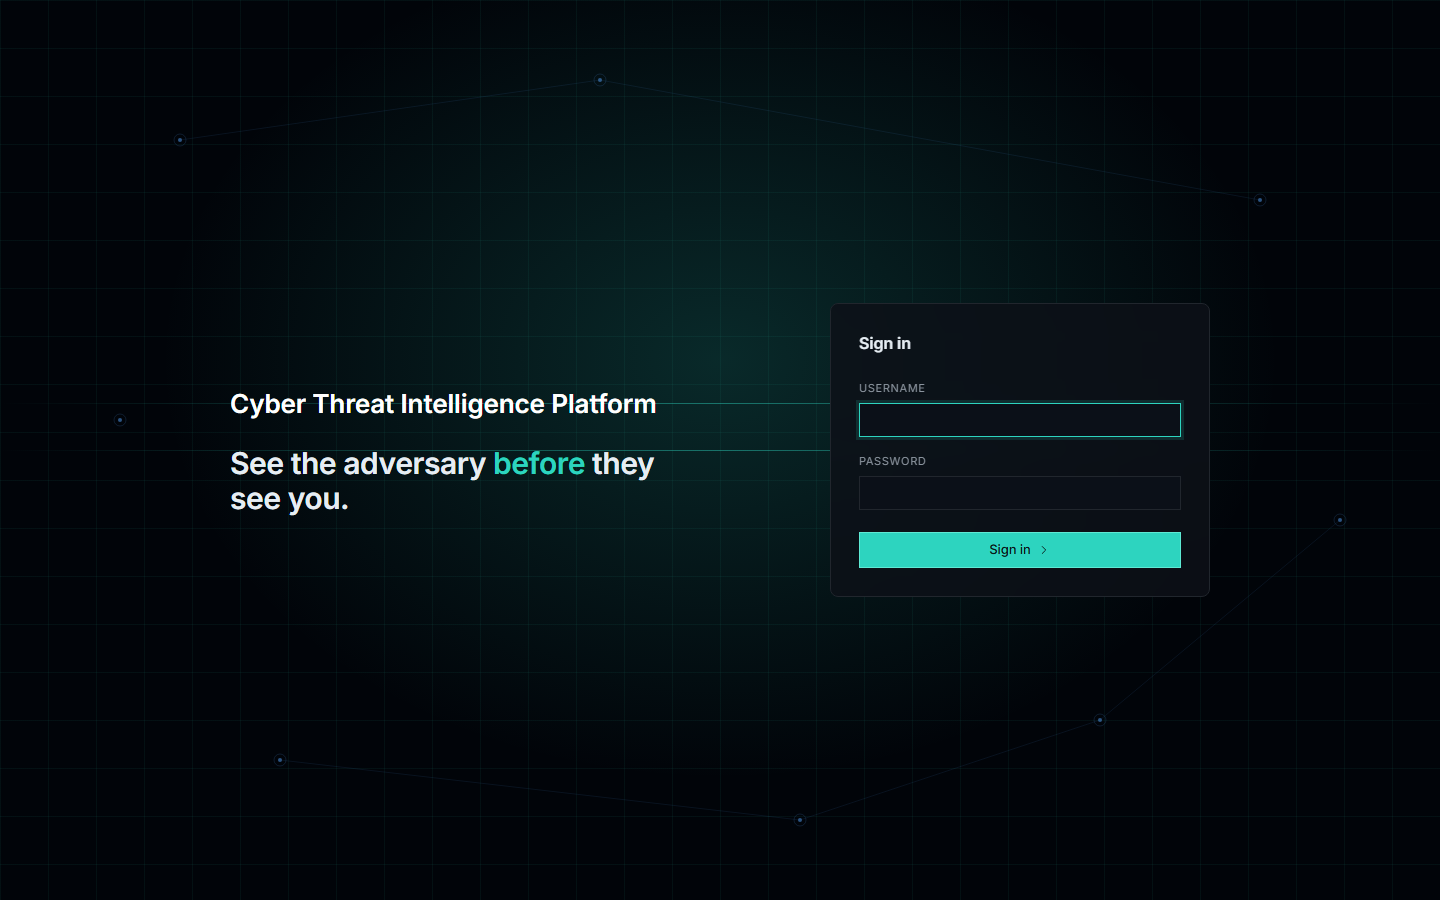
\includegraphics[width=0.82\textwidth]{images/tip/shots/01_login.png}
\caption{Login workflow entry point.}
\label{fig:login-workflow}
\end{figure}

\subsection{Dashboard Consumption}
The dashboard workflow is an aggregation workflow. The user expects a single situational view, but the backend knowledge required to produce that view comes from many services. The BFF therefore collects and reshapes the relevant data before returning it to the page.

\begin{figure}[H]
\centering
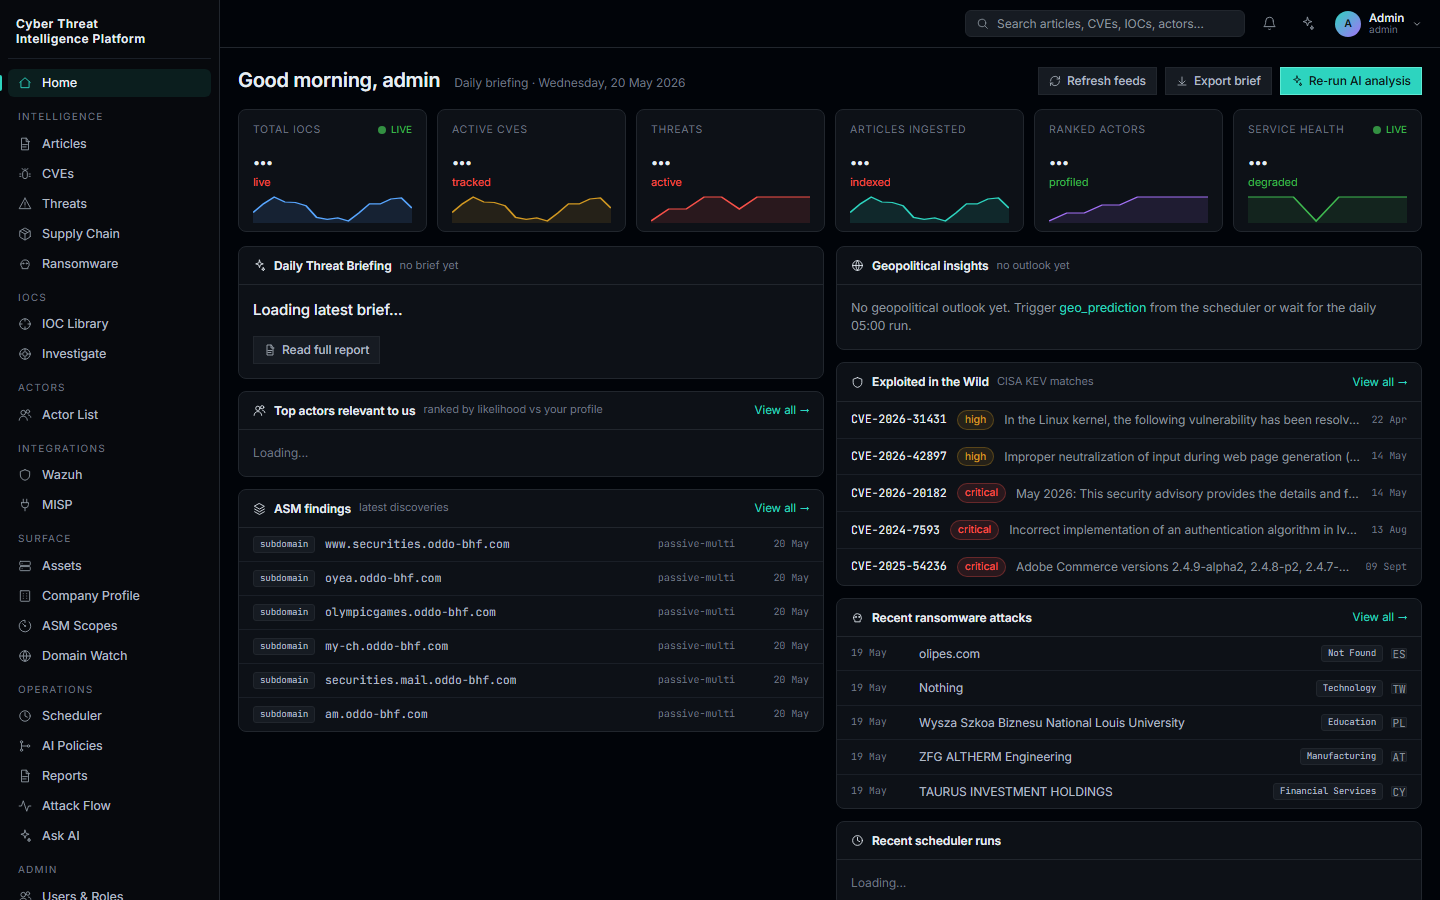
\includegraphics[width=0.9\textwidth]{images/tip/shots/02_dashboard.png}
\caption{Dashboard workflow as a composed intelligence surface.}
\label{fig:dashboard-workflow}
\end{figure}

\subsection{Article Review and Enrichment}
Article browsing and article detail workflows show how narrative reporting is converted into locally usable intelligence. The analyst can move from a list of ingested articles to deeper detail and associated insights.

\begin{figure}[H]
\centering
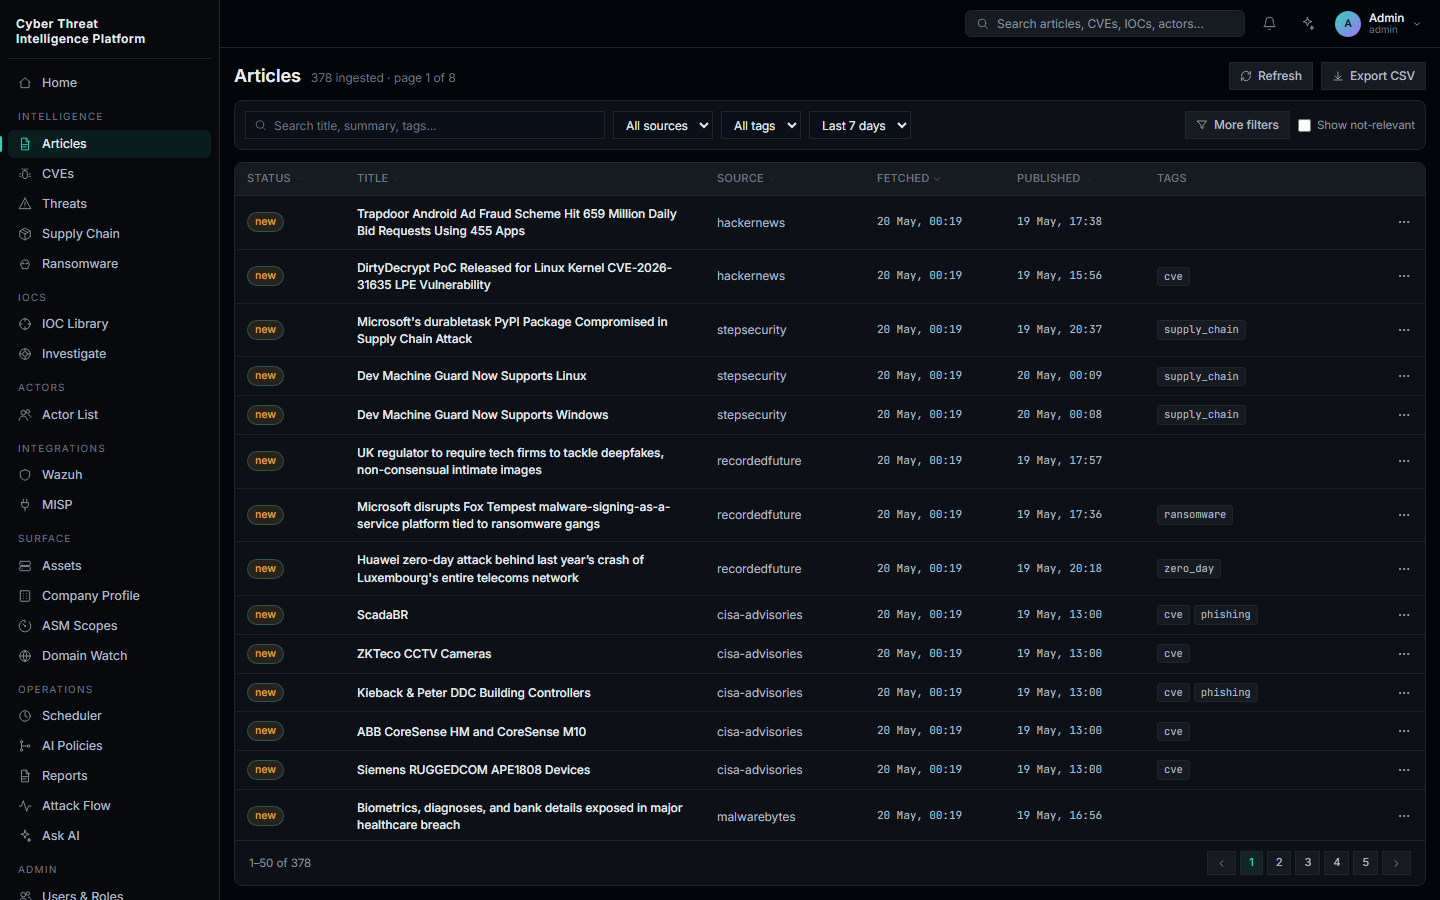
\includegraphics[width=0.9\textwidth]{images/tip/shots/03_articles_list.png}
\caption{Article-list workflow.}
\label{fig:article-list-workflow}
\end{figure}

\begin{figure}[H]
\centering
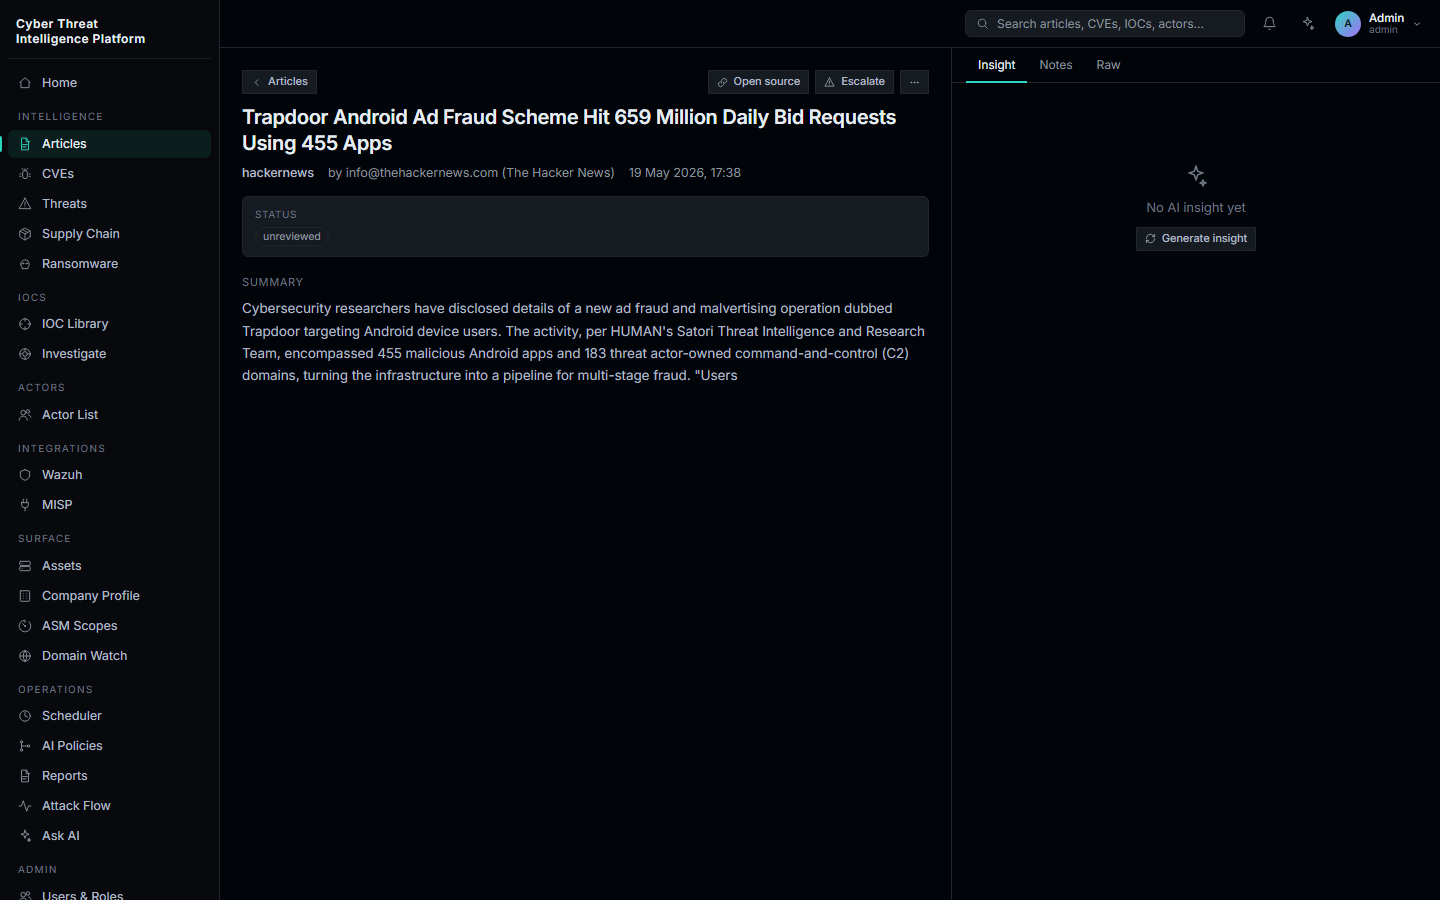
\includegraphics[width=0.9\textwidth]{images/tip/shots/04_article_detail.png}
\caption{Article-detail workflow.}
\label{fig:article-detail-workflow}
\end{figure}

\subsection{Vulnerability Prioritization Workflow}
The CVE list and CVE detail views represent one of the platform's most important analytical surfaces. They do not merely expose a feed. They provide a context in which vulnerabilities can be interpreted relative to exploitability and local relevance.

\begin{figure}[H]
\centering
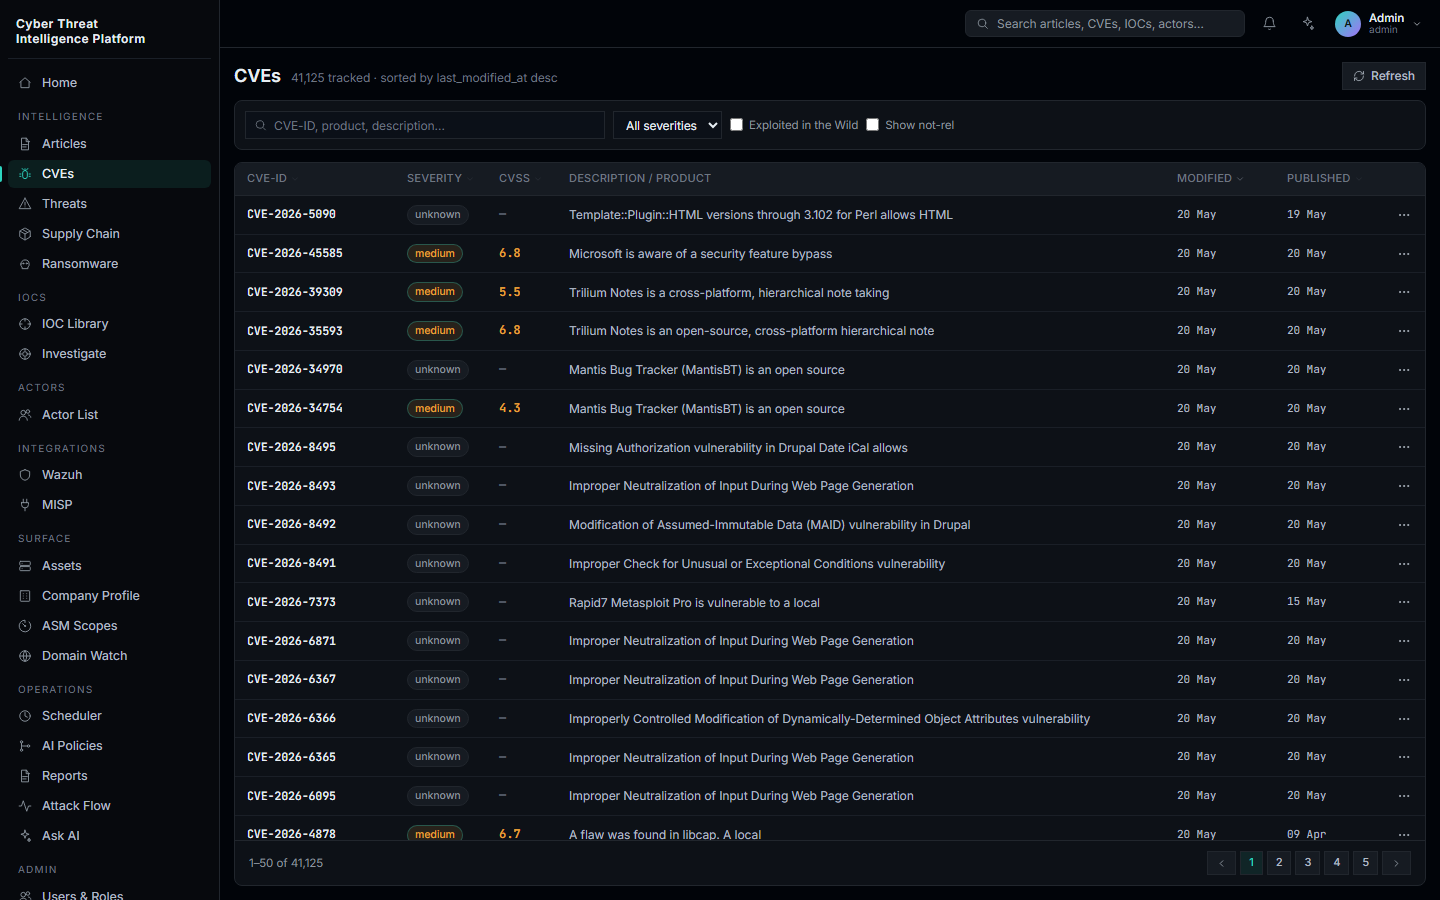
\includegraphics[width=0.88\textwidth]{images/tip/shots/06_cves_list.png}
\caption{Vulnerability-list workflow.}
\label{fig:cves-list-workflow}
\end{figure}

\begin{figure}[H]
\centering
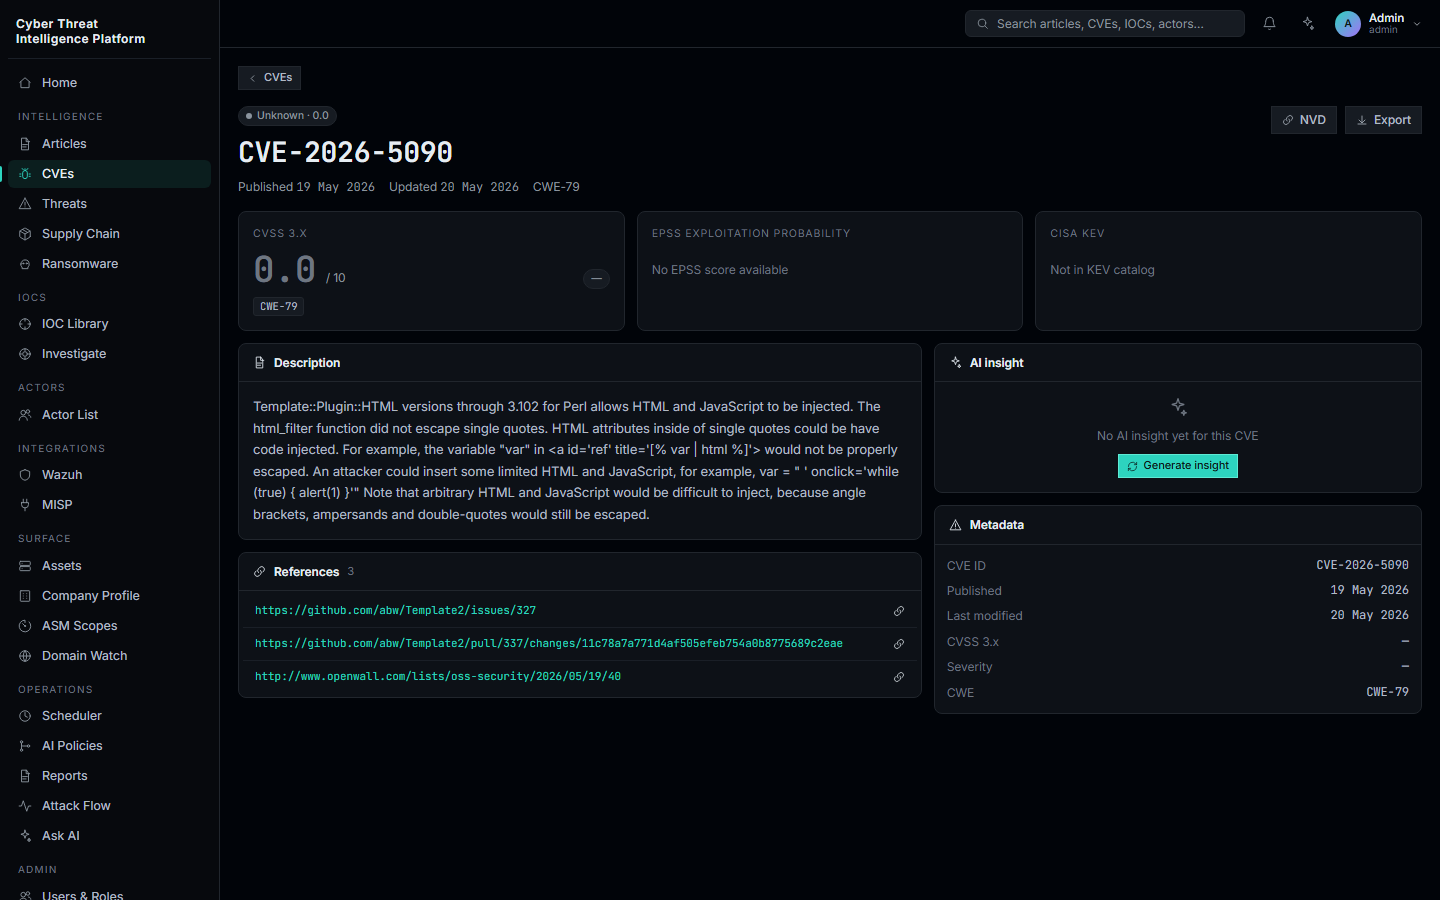
\includegraphics[width=0.88\textwidth]{images/tip/shots/07_cve_detail.png}
\caption{Vulnerability-detail workflow.}
\label{fig:cve-detail-workflow}
\end{figure}

\subsection{Threat and Actor Exploration}
Threat exploration workflows support higher-level intelligence interpretation. Analysts can move from lists of threats or actors to profiles, TTP associations, and AI-generated analytical tabs.

\begin{figure}[H]
\centering
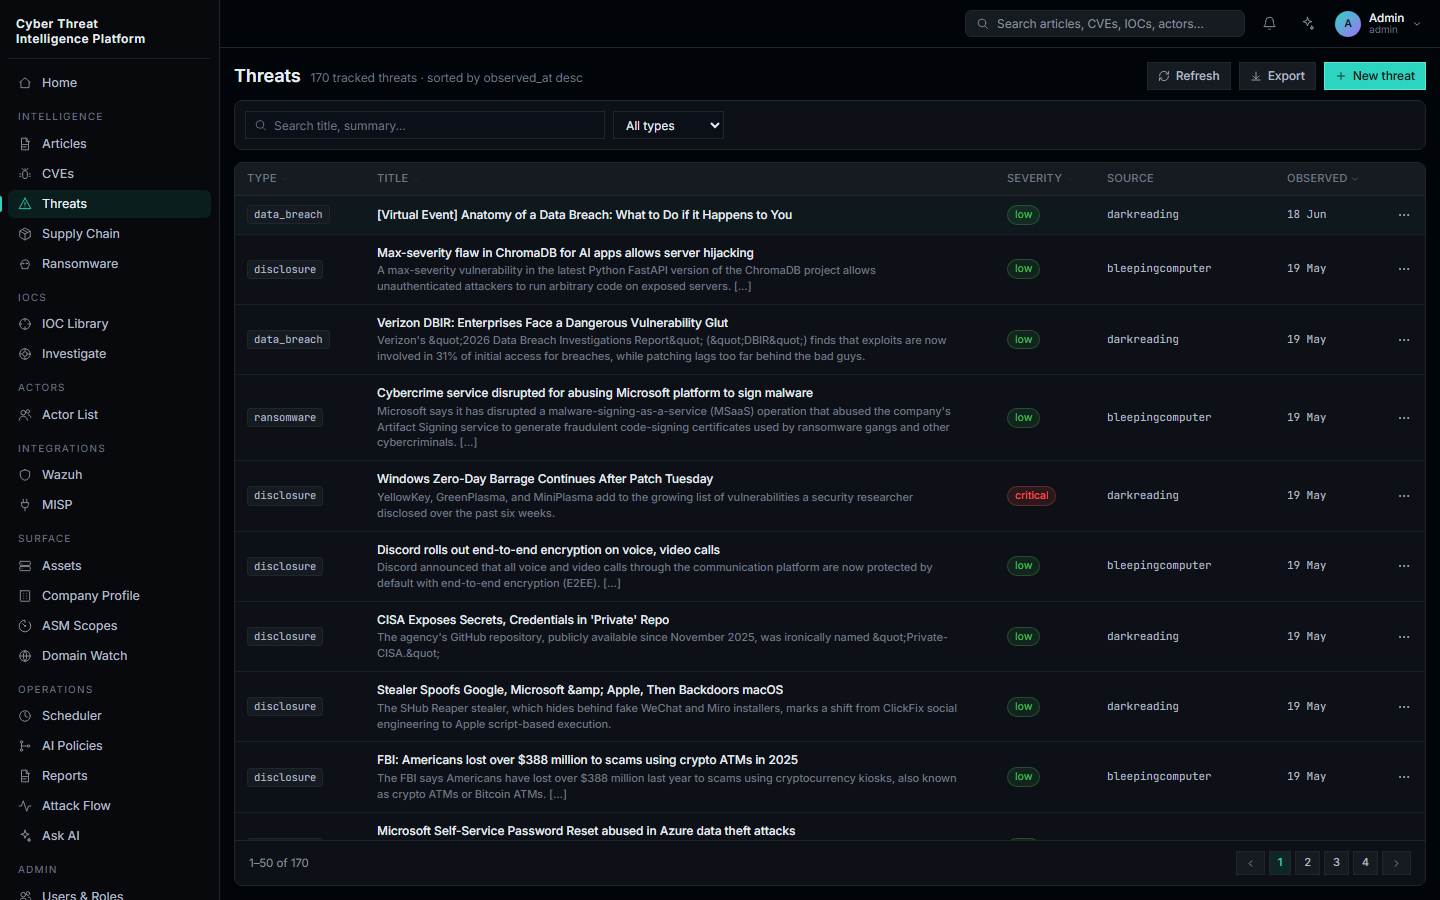
\includegraphics[width=0.88\textwidth]{images/tip/shots/08_threats_list.png}
\caption{Threat-list workflow.}
\label{fig:threat-list-workflow}
\end{figure}

\begin{figure}[H]
\centering
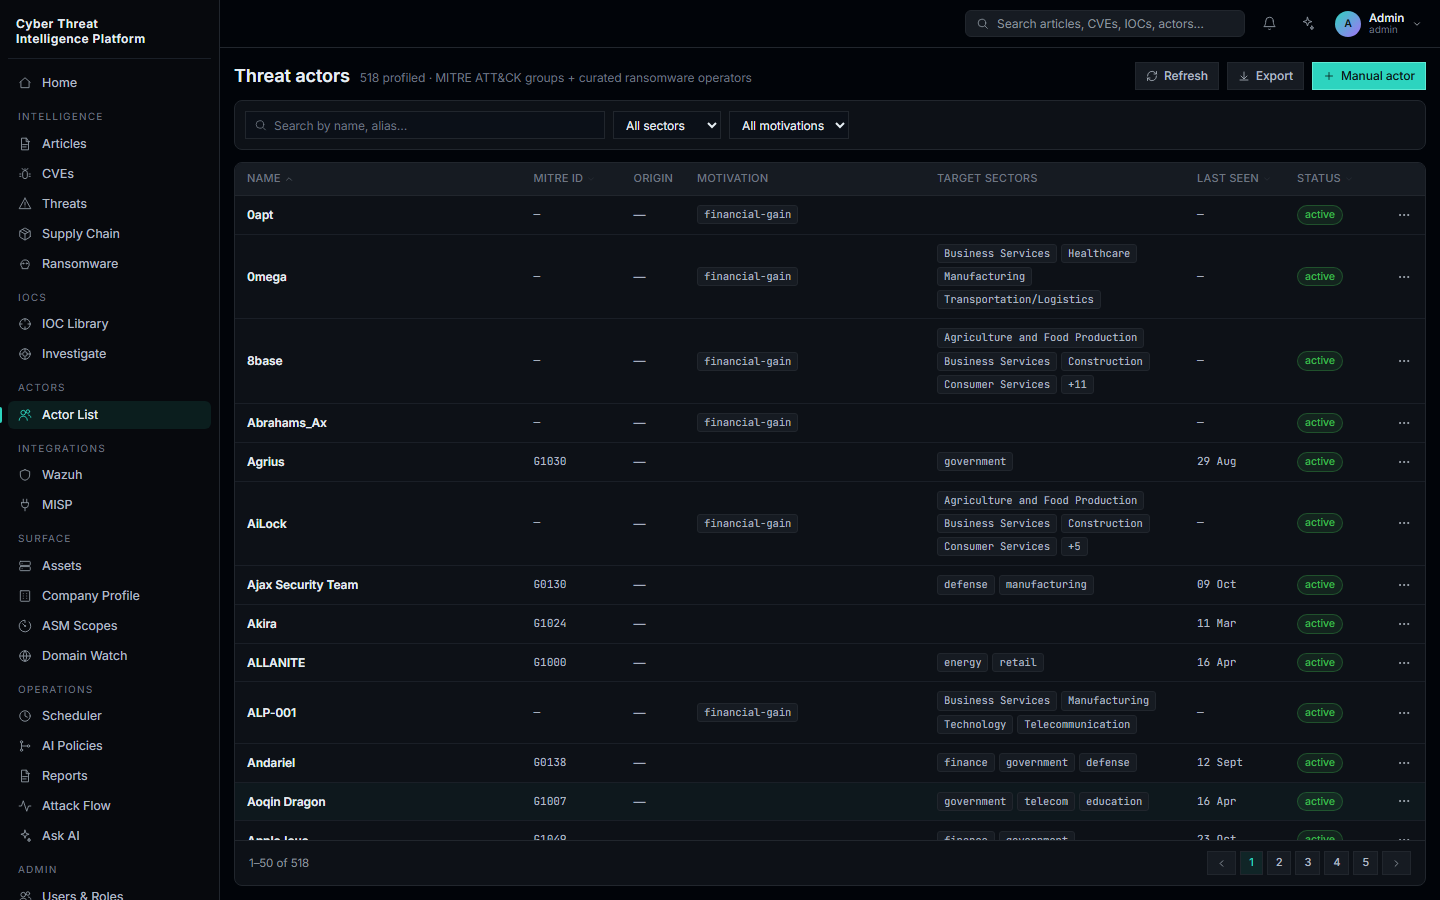
\includegraphics[width=0.88\textwidth]{images/tip/shots/18_actors_list.png}
\caption{Threat-actor list workflow.}
\label{fig:actors-list-workflow}
\end{figure}

\begin{figure}[H]
\centering
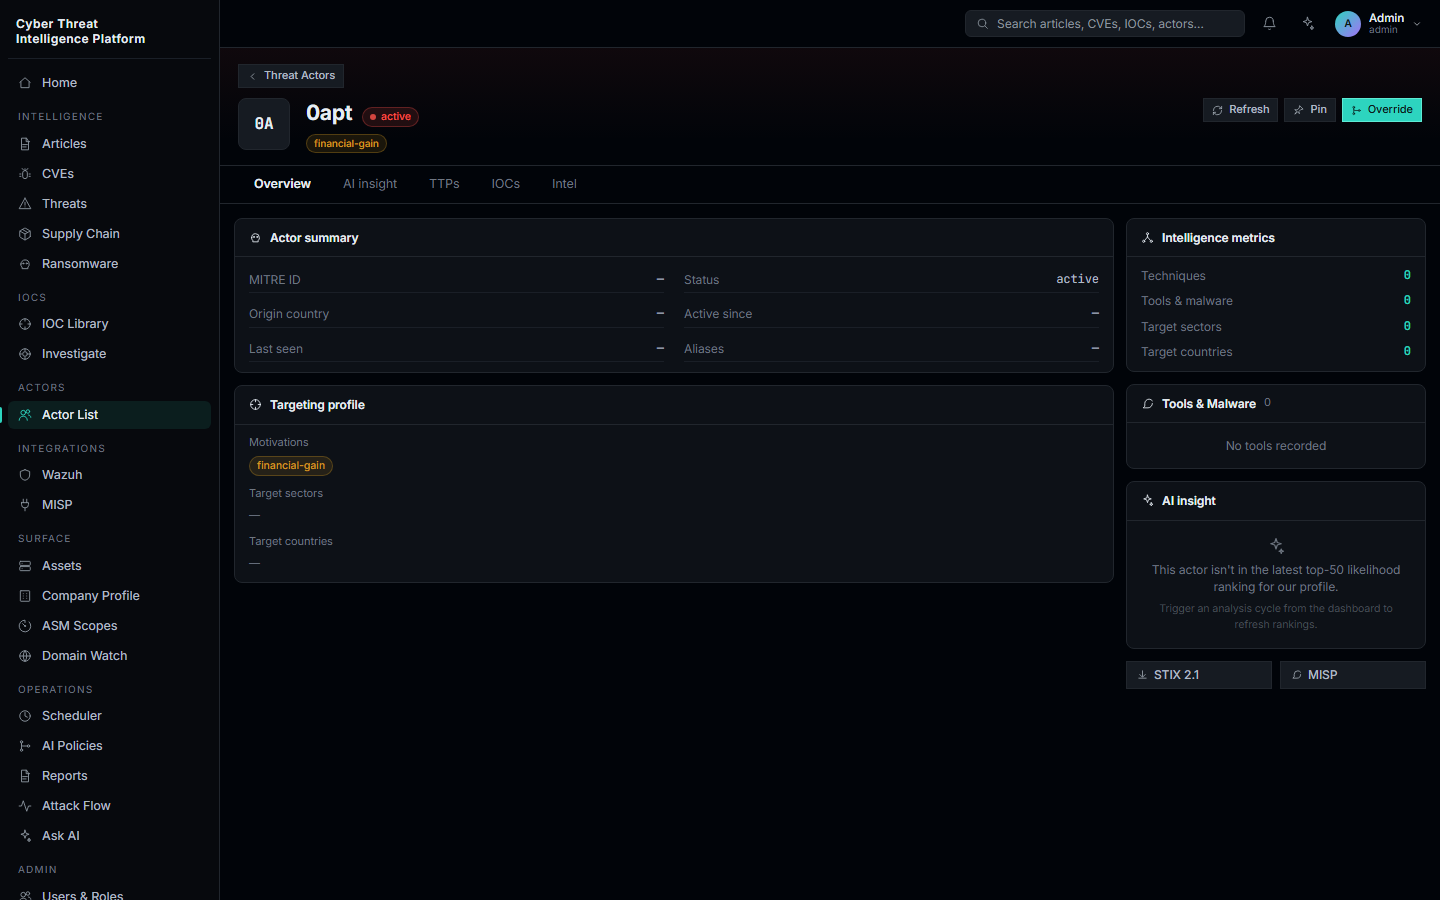
\includegraphics[width=0.88\textwidth]{images/tip/shots/19_actor_profile_overview.png}
\caption{Threat-actor profile workflow.}
\label{fig:actor-profile-workflow}
\end{figure}

\subsection{IOC Investigation Workflow}
The IOC workflow demonstrates the platform's dual-path design particularly well. The analyst can move from quick lookup to deeper investigation, with the latter using broader local and passive context.

\begin{figure}[H]
\centering
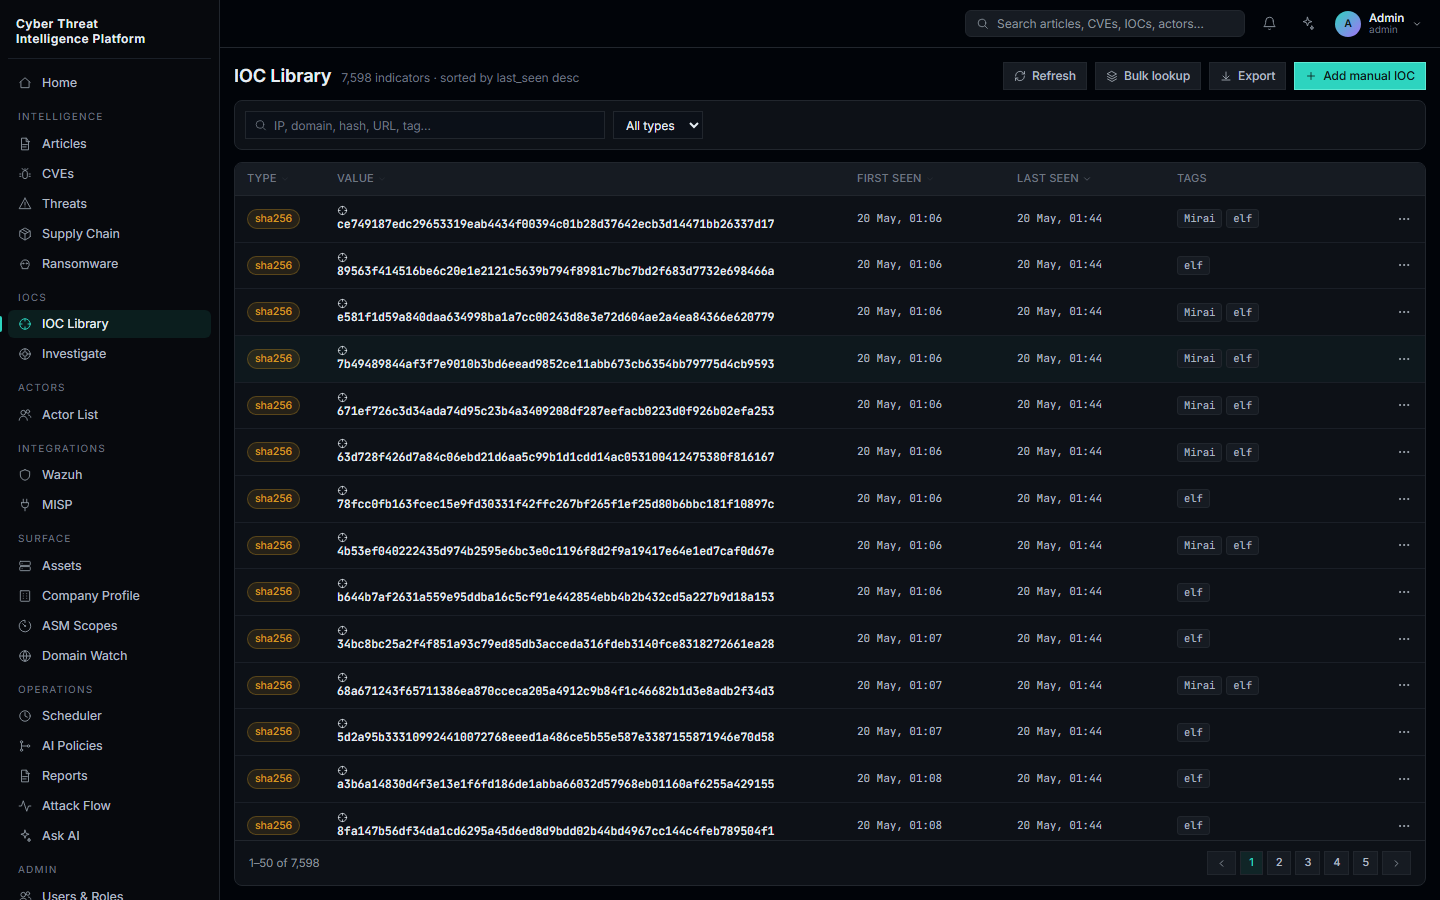
\includegraphics[width=0.88\textwidth]{images/tip/shots/13_iocs_library.png}
\caption{IOC-library workflow.}
\label{fig:ioc-library-workflow}
\end{figure}

\begin{figure}[H]
\centering
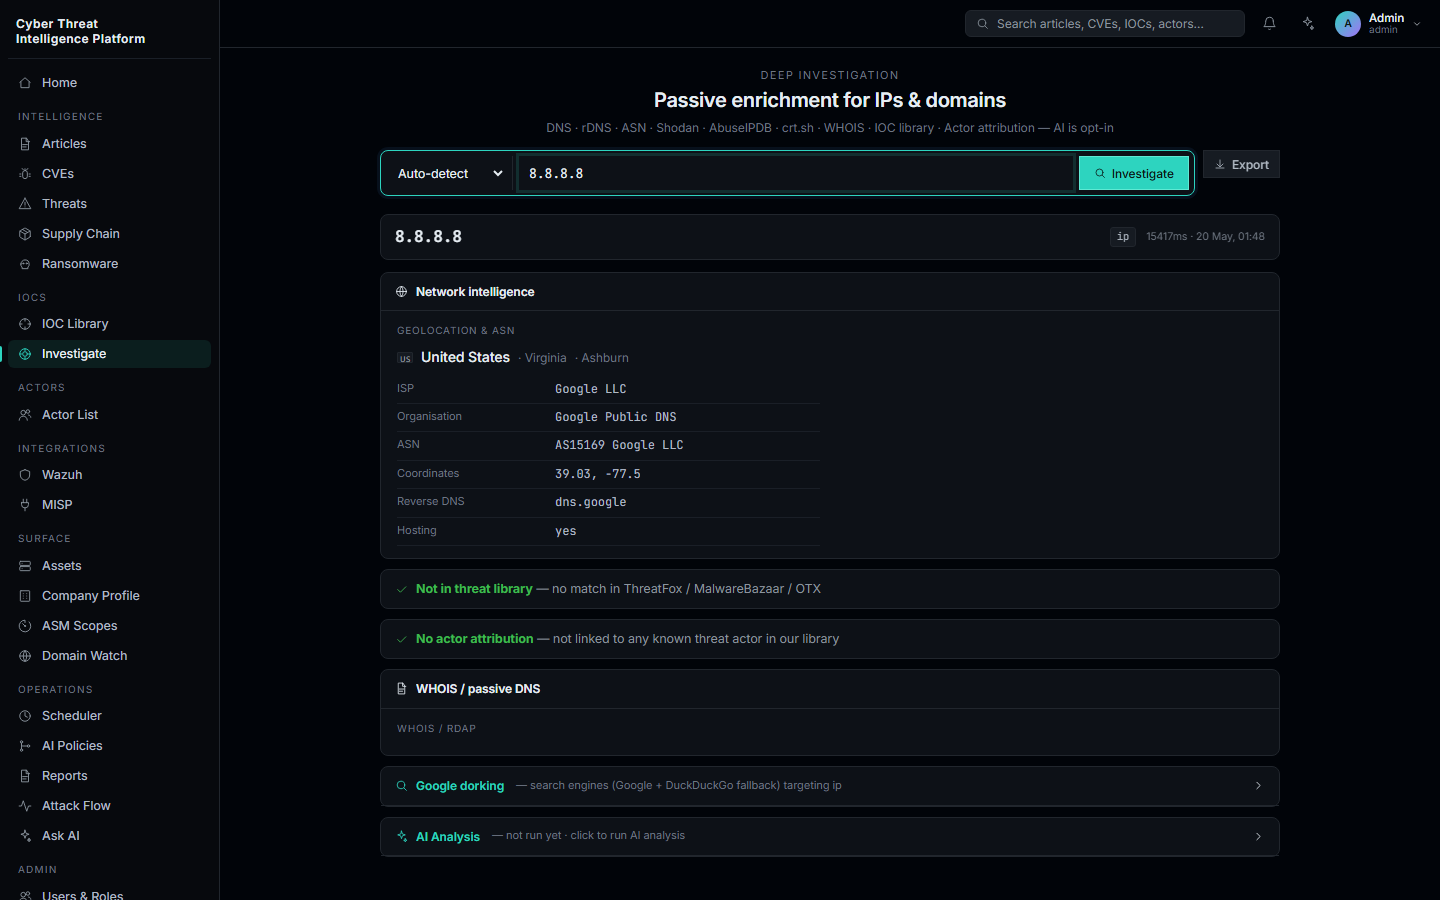
\includegraphics[width=0.88\textwidth]{images/tip/shots/16_ioc_investigate_result.png}
\caption{Deep IOC-investigation workflow.}
\label{fig:ioc-investigation-workflow}
\end{figure}

\subsection{Asset and Organization Context Workflow}
The asset and company-profile workflow is what allows the platform to move beyond generic feed consumption. It gives the system a local referent: which technologies, profiles, and exposures are actually relevant to the organization.

\begin{figure}[H]
\centering
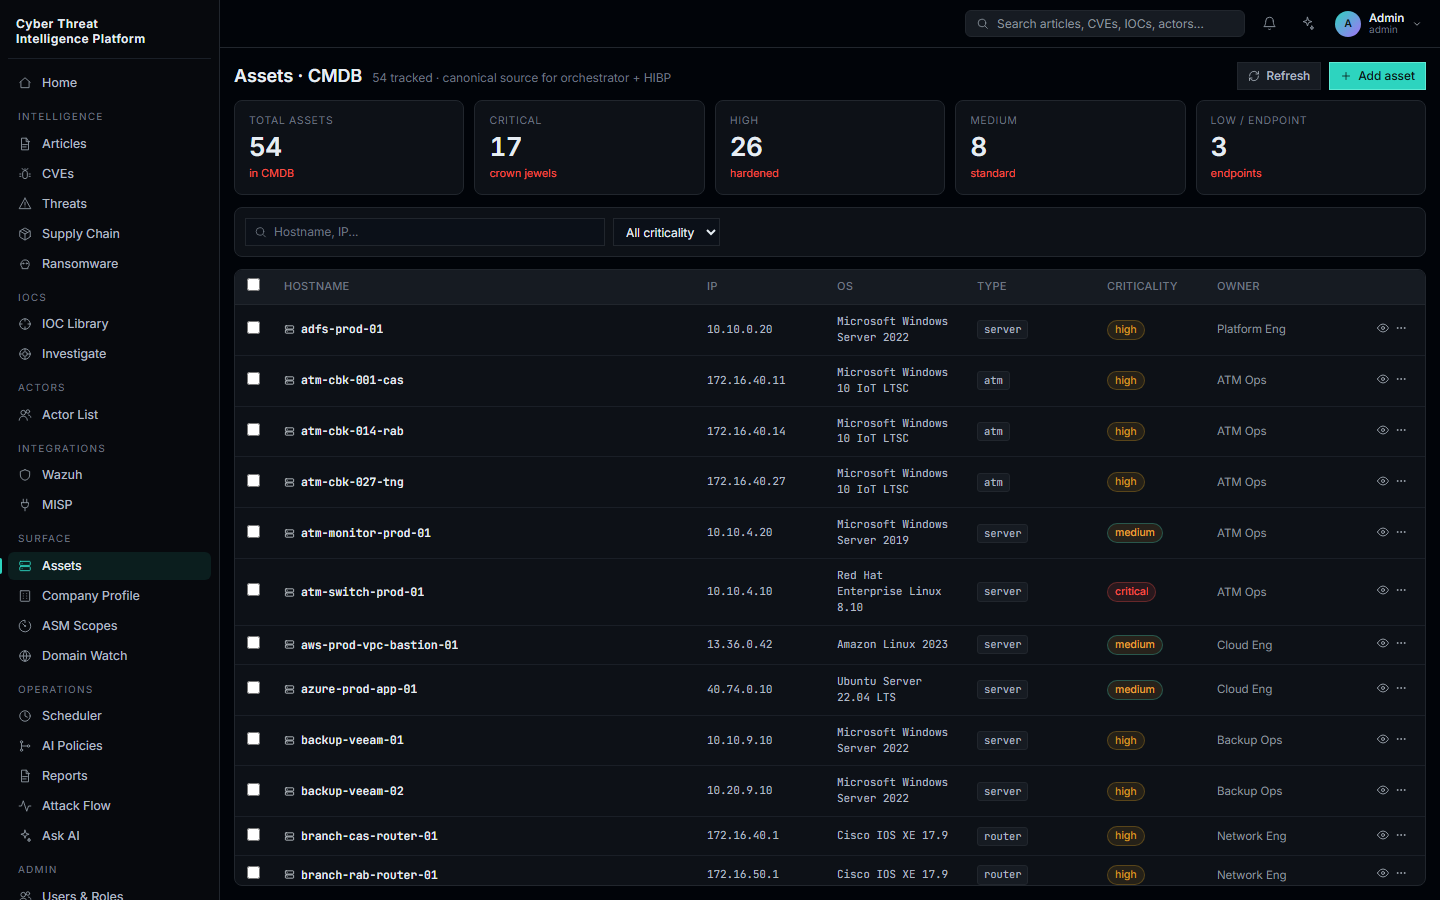
\includegraphics[width=0.88\textwidth]{images/tip/shots/22_assets_list.png}
\caption{Asset-list workflow.}
\label{fig:assets-list-workflow}
\end{figure}

\begin{figure}[H]
\centering
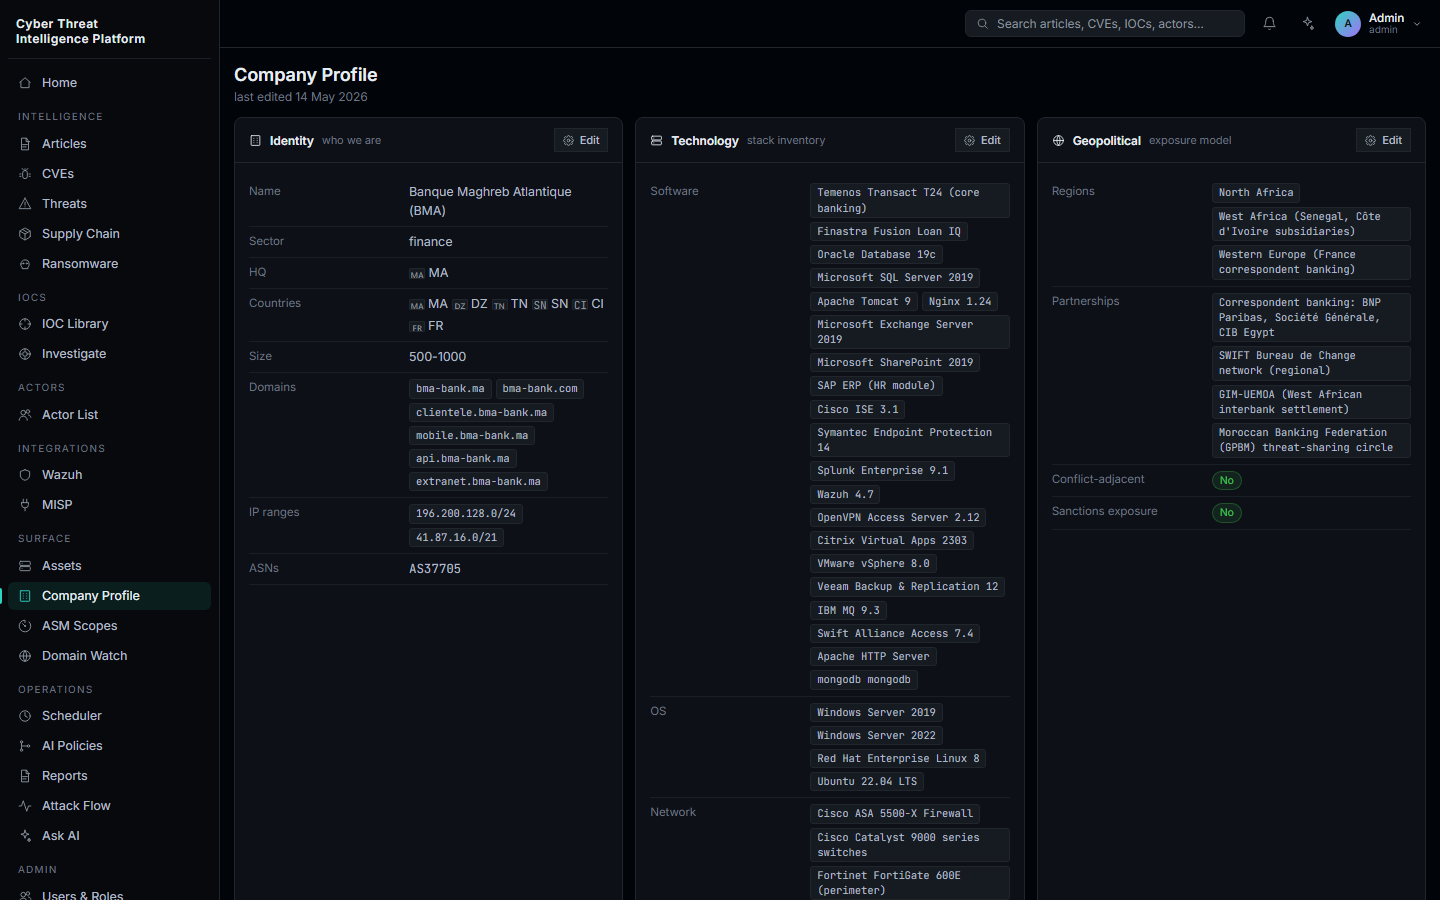
\includegraphics[width=0.88\textwidth]{images/tip/shots/23_assets_company_profile.png}
\caption{Company-profile workflow.}
\label{fig:company-profile-workflow}
\end{figure}

\subsection{Reports, Policies, and Administrative Workflows}
The reports, AI policies, settings, and administration pages show that the platform is not just an analyst sandbox. It is also a managed operational system with governance surfaces.

\begin{figure}[H]
\centering
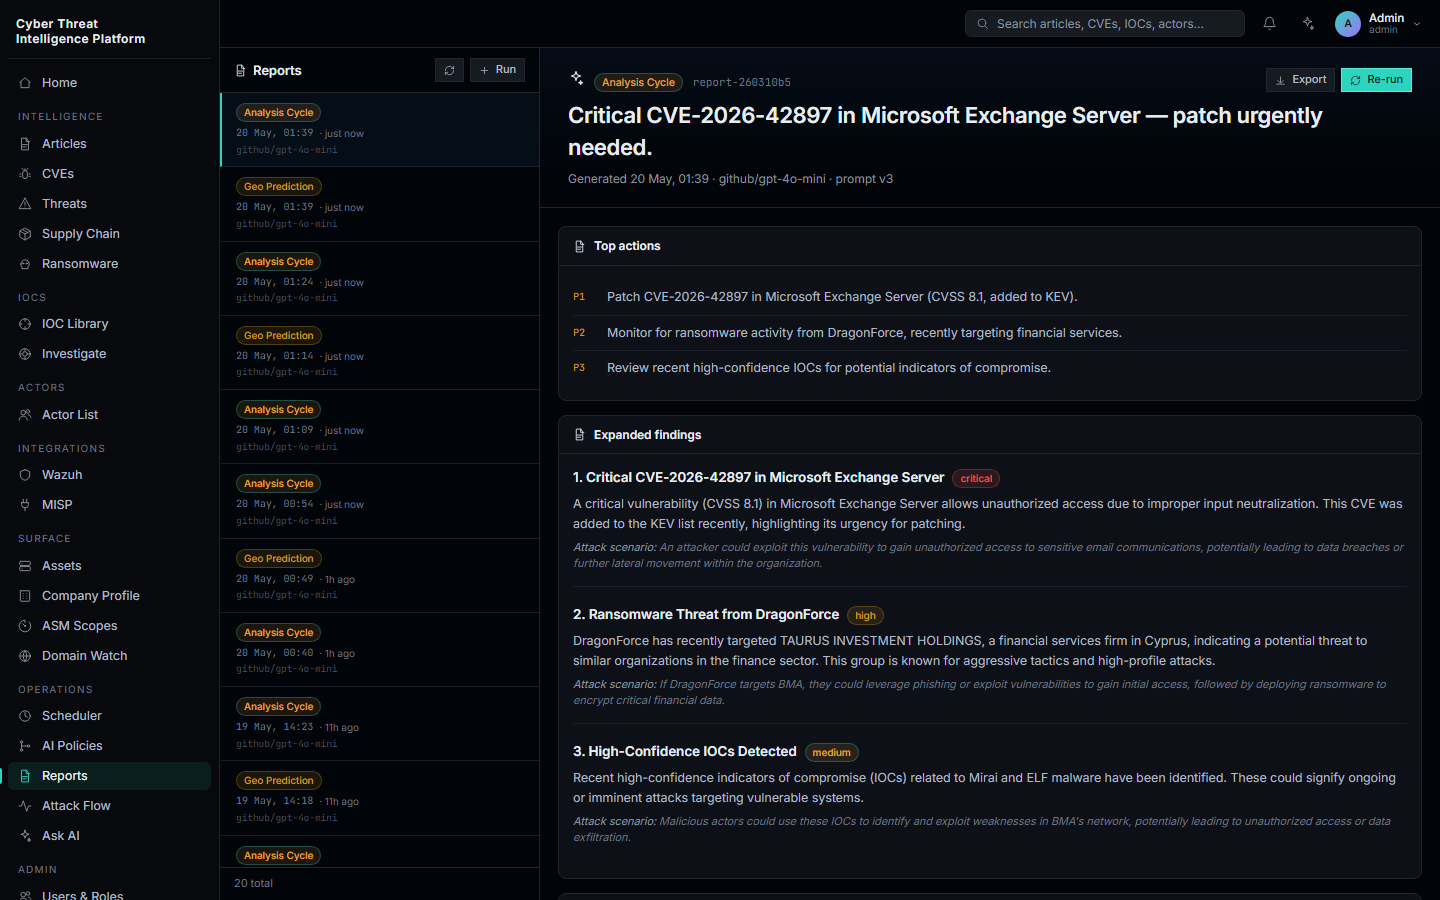
\includegraphics[width=0.88\textwidth]{images/tip/shots/31_reports.png}
\caption{Reports workflow.}
\label{fig:reports-workflow}
\end{figure}

\begin{figure}[H]
\centering
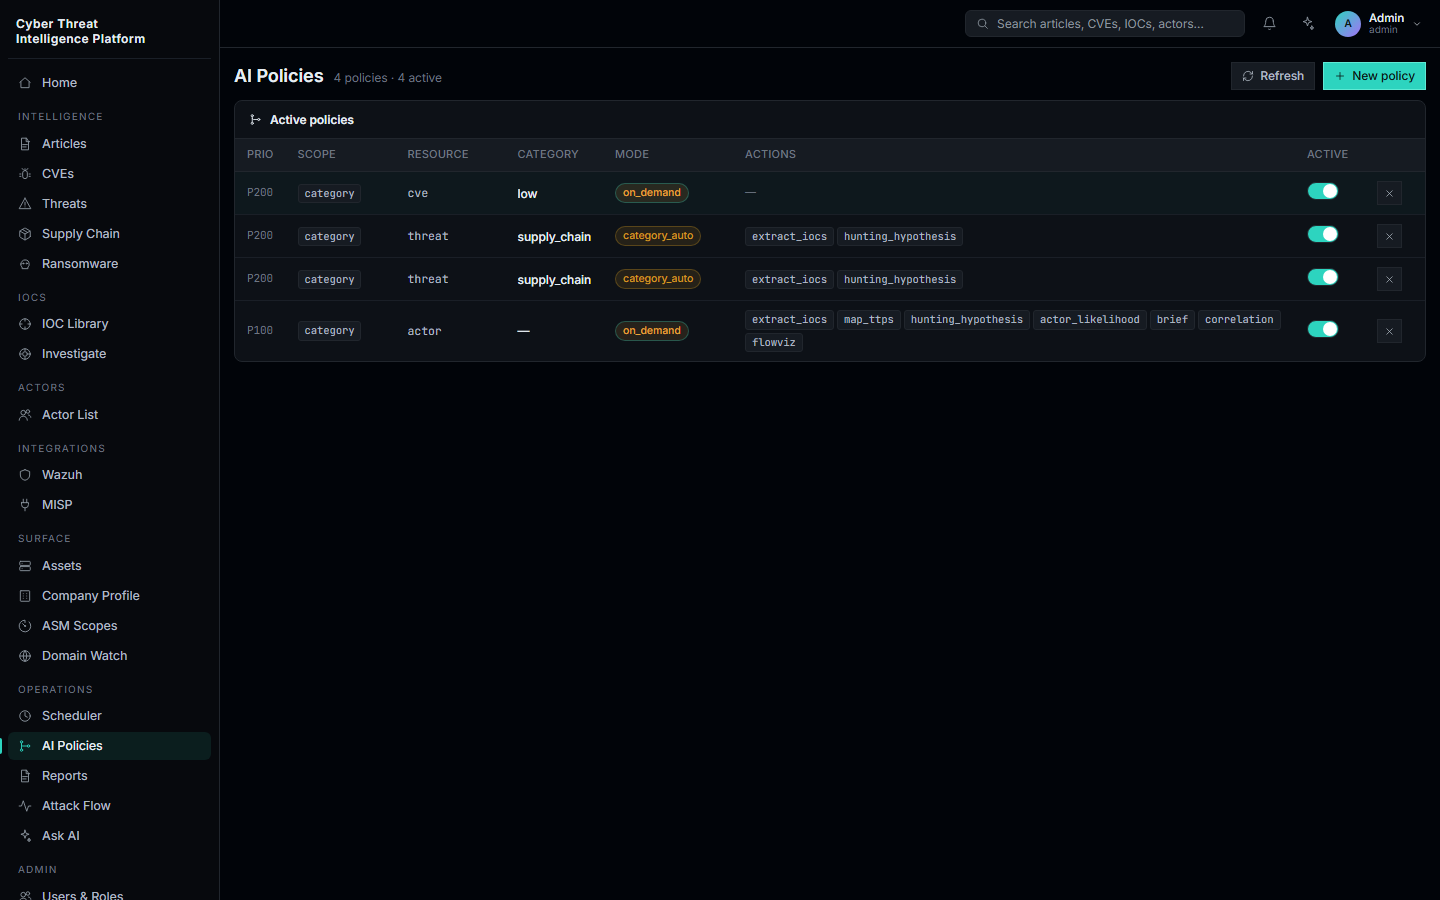
\includegraphics[width=0.88\textwidth]{images/tip/shots/30_ai_policies.png}
\caption{AI-policy workflow.}
\label{fig:ai-policy-workflow}
\end{figure}

\begin{figure}[H]
\centering
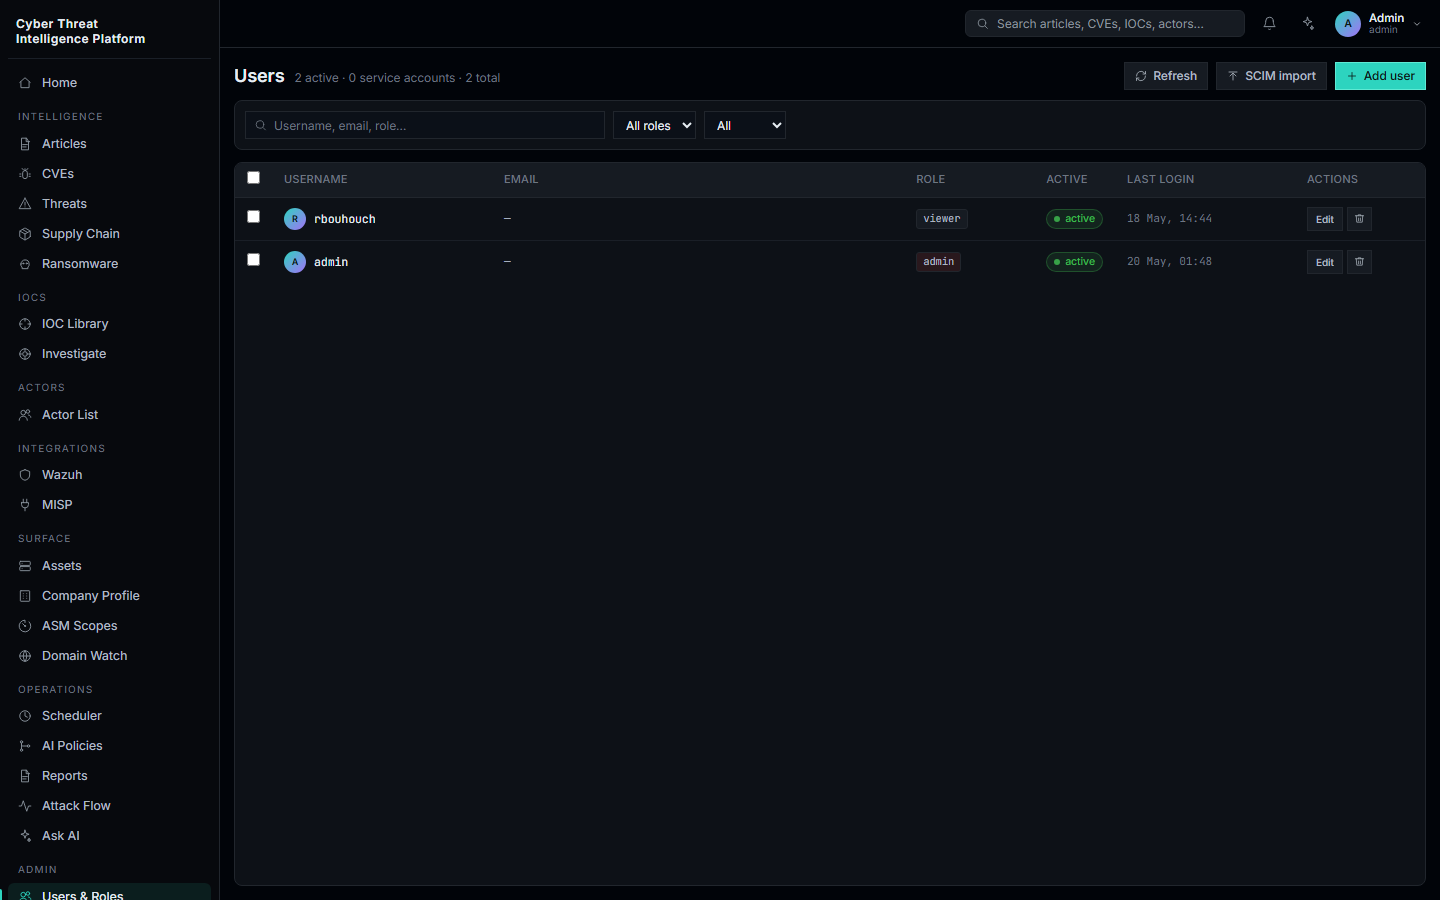
\includegraphics[width=0.88\textwidth]{images/tip/shots/34_admin_users.png}
\caption{Administrative user-management workflow.}
\label{fig:admin-users-workflow}
\end{figure}

\section{Why the Frontend Matters Architecturally}
It is tempting to treat the frontend as presentation only and therefore secondary in an architecture chapter. That would be a mistake here. The frontend determines how quickly analysts can convert platform capability into operational action. It also hosts the BFF, which means it participates directly in routing, aggregation, and edge trust. In this system, the frontend is therefore part of the architecture, not merely a decorative layer over it.

\section*{Conclusion}
\addcontentsline{toc}{section}{Conclusion}
The platform's data model, API design, and frontend workflows form one coherent chain. The data model defines what can be stored and correlated. The API layer defines how that knowledge is exposed and governed. The frontend defines how analysts and managers actually consume and act on the result. Understanding all three is necessary to understand why the platform works as an operational tool rather than only as a backend service collection.

\chapter{Implementation, Runtime Behaviour, and Operations}
\thispagestyle{plain}
\section*{Introduction}
\addcontentsline{toc}{section}{Introduction}
This chapter explains how the architecture executes in practice. It covers the shared backend skeleton, the runtime startup sequence, database and cache usage, asynchronous workflows, AI-assisted analysis paths, deployment mechanics, observability, resilience, performance characteristics, and representative features exposed through the user interface.

\section{Implementation Philosophy}
Implementation choices in this project were not made solely for code elegance. They were driven by a recurring tension between correctness, latency, operability, and dependency fragility. A useful way to read the implementation is therefore to distinguish essential complexity from accidental complexity. Essential complexity comes from the problem domain itself: many feeds, many entity types, partial failure, context-sensitive prioritization, and AI-assisted summarization. Accidental complexity comes from avoidable inconsistency, duplicate infrastructure logic, ad hoc configuration, and uncontrolled side effects.

Much of the repository's engineering discipline is aimed at reducing accidental complexity. Shared factories, shared libraries, uniform transaction boundaries, and explicit startup hooks do not make the domain simpler, but they do make the codebase more predictable. That predictability is academically relevant because it is one of the main preconditions for maintainability in a multi-service system.

\section{The Shared Backend Skeleton}
The most important implementation pattern in the repository is that all services share one application factory. The factory sets up structured logging, correlation IDs, health checks, and error handling; each service then adds its own routers and startup hooks.

\begin{lstlisting}[caption={Shared service factory excerpt},label={lst:factory-new}]
def create_service_app(*, settings, title, description="",
                       on_startup=None, on_shutdown=None):
    configure_logging(settings.service_name, settings.log_level)
    app = FastAPI(title=title, version="0.1.0", lifespan=lifespan)
    app.add_middleware(CorrelationIdMiddleware)
    register_error_handlers(app)
    @app.get("/health")
    async def health():
        return {"status": "ok", "service": settings.service_name}
    return app
\end{lstlisting}

The omission is as important as the inclusion: JWT middleware is not wired in the factory because key retrieval happens during startup. This small decision prevents premature configuration coupling between service import time and runtime secret availability.

The broader implementation lesson is that lifecycle order matters. In distributed applications, it is often incorrect to assume that everything required by request-time logic is already available at import time. The repository explicitly models startup as a separate phase in which secrets, keys, pools, caches, and clients are acquired. This yields a more accurate program structure than pretending initialization and steady-state request handling are the same kind of work.

\section{Startup Lifecycle and Runtime State}
The per-service startup flow follows a repeatable pattern: initialize the async SQLAlchemy engine, create or obtain a session factory, attach a Redis cache if the service uses one, construct a secrets client when startup secrets are required, build AI clients only in services that need them, create source-health repositories only in services that talk to external sources, then wire auth bootstrap.

Figures~\ref{fig:runtime-flow-new} and \ref{fig:runtime-flow-bottom} summarize the sequence.

\begin{figure}[H]
\centering
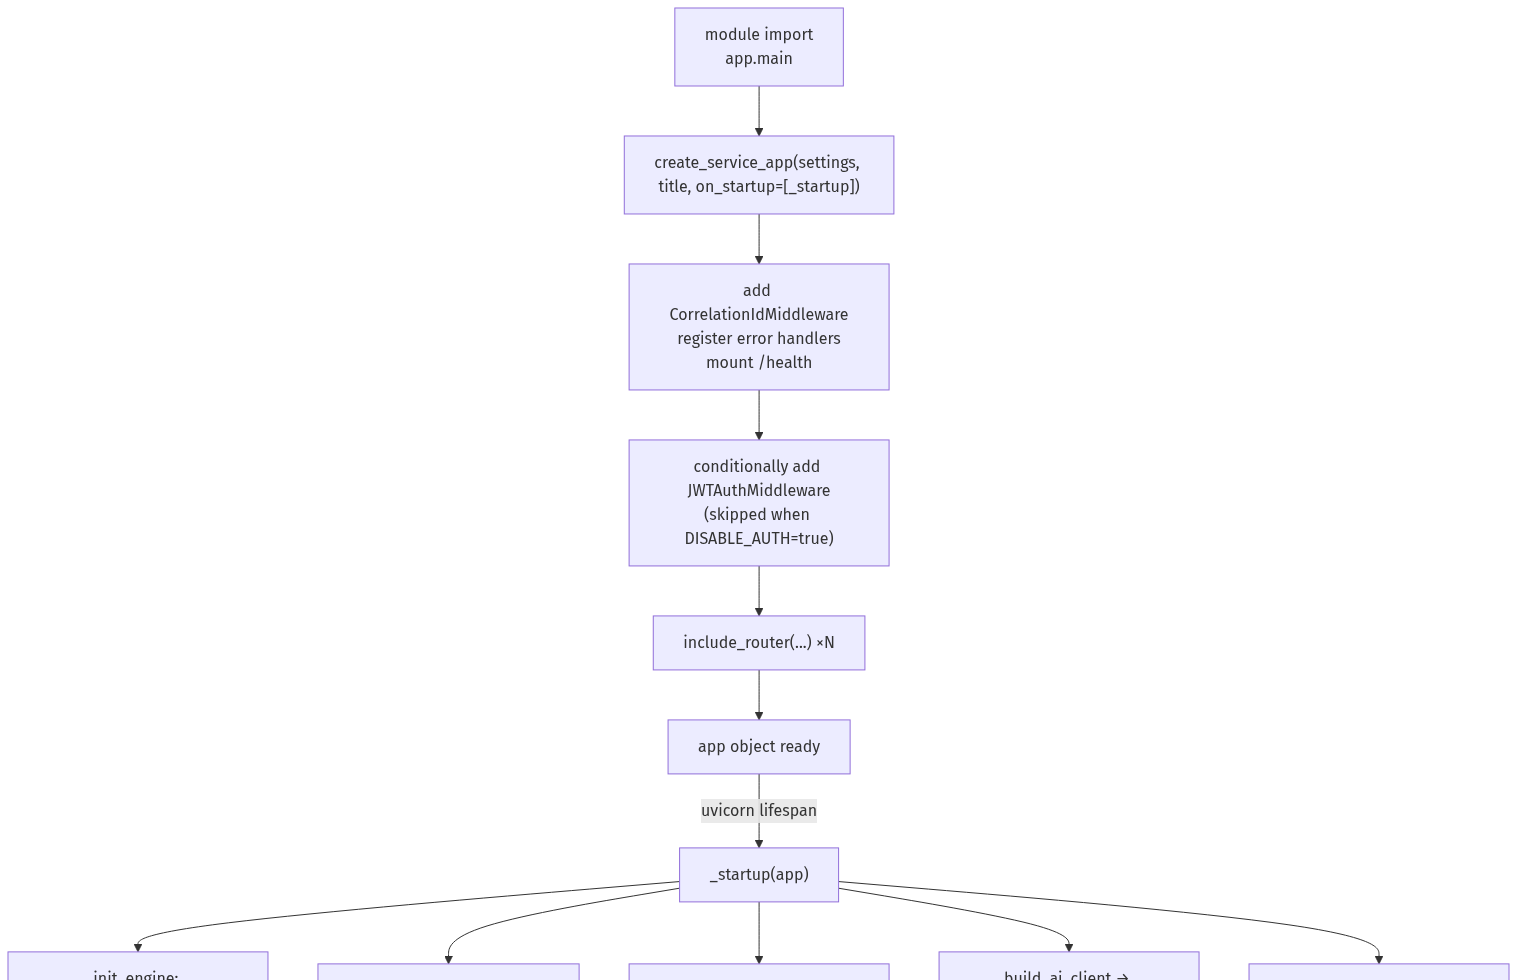
\includegraphics[width=0.92\textwidth]{images/tip/diagrams/10_runtime_flow_top.png}
\caption{Service runtime flow from startup hooks to request handling, upper segment.}
\label{fig:runtime-flow-new}
\end{figure}

\begin{figure}[H]
\centering
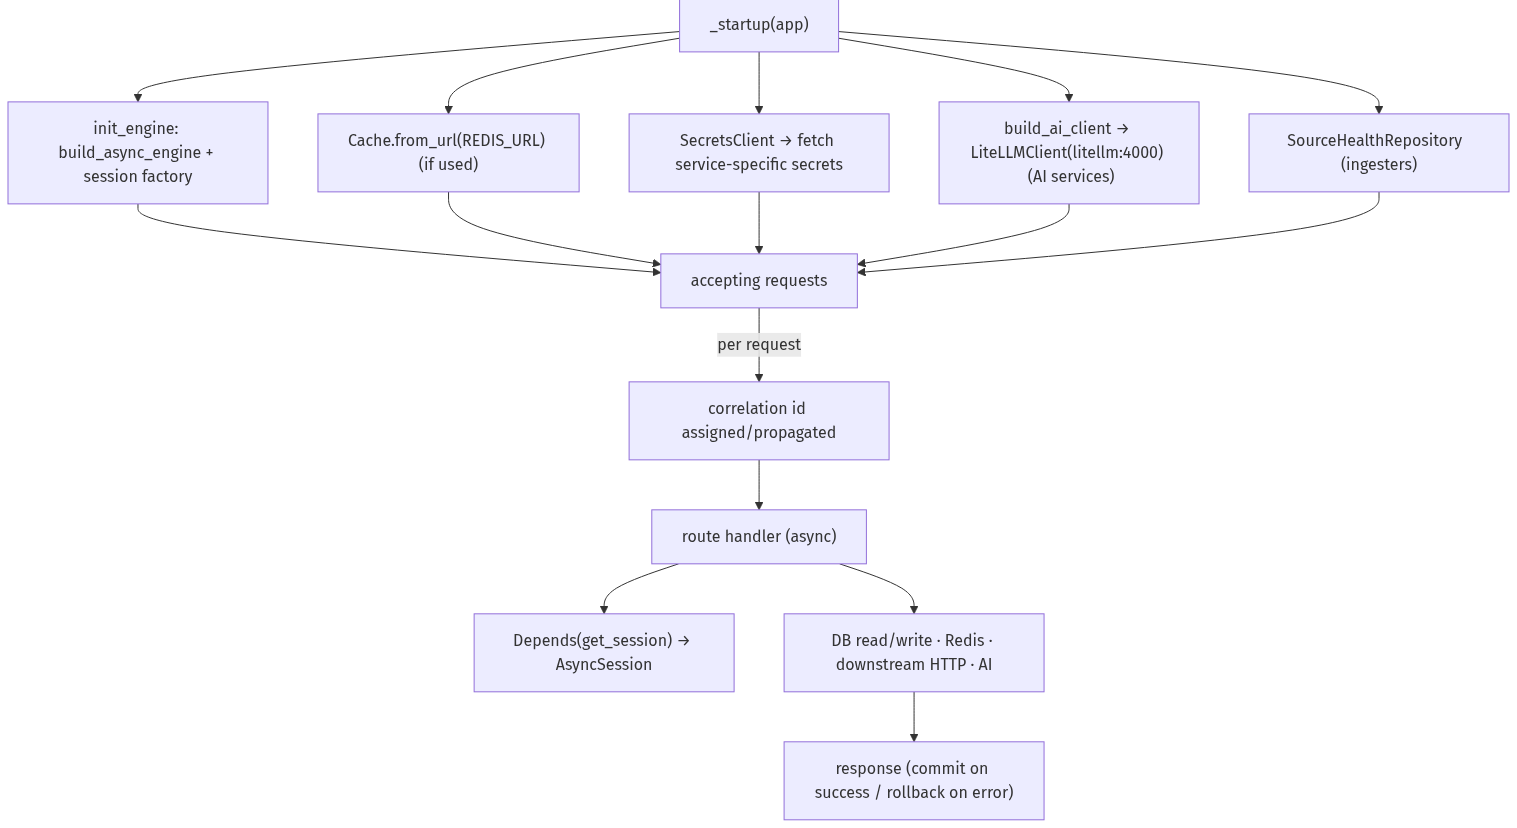
\includegraphics[width=0.92\textwidth]{images/tip/diagrams/10_runtime_flow_bottom.png}
\caption{Service runtime flow from startup hooks to request handling, lower segment.}
\label{fig:runtime-flow-bottom}
\end{figure}

This pattern offers a useful compromise. Shared operational concerns are centralized, but runtime capability remains opt-in. A simple CRUD-style service does not carry the cost of the full AI stack, while an ingest service can attach health tracking and resilient HTTP without duplicating infrastructure code.

From a software design perspective, this is a form of capability-based composition. A service acquires only the runtime components needed for its actual role. This reduces unnecessary transitive complexity and limits the number of active failure paths in simpler services. It also makes the service graph easier to reason about because optional capabilities are visible during startup rather than hidden in always-on global state.

\section{Database Access and Transaction Boundaries}
Database access is implemented with async SQLAlchemy sessions wrapped in a dependency that commits on success and rolls back on failure.

\begin{lstlisting}[caption={Per-request transaction boundary},label={lst:session-new}]
async def get_session(factory):
    async with factory() as session:
        try:
            yield session
            await session.commit()
        except Exception:
            await session.rollback()
            raise
\end{lstlisting}

This implementation has two notable consequences. First, route handlers stay focused on domain logic rather than transaction management. Second, service-wide behaviour is consistent, which matters in a multi-service monorepo where inconsistent transaction boundaries would be difficult to reason about.

There is also an important correctness property here. By placing commit and rollback responsibility in one shared dependency, the repository reduces the risk of partially applied request logic caused by handler-local transaction management. In practical terms, this means the developer is less likely to forget to commit, over-commit, or leak transaction scope across unrelated operations.

\section{Resilient Outbound Communication}
Every external call is assumed to be fallible. The shared resilience layer provides retry policy, retryability rules, timeout handling, and circuit-state integration with source health. The retry policy itself is intentionally modest: three attempts, exponential backoff, and jitter.

\begin{lstlisting}[caption={Retry policy for external source calls},label={lst:retry-new}]
@dataclass
class RetryPolicy:
    max_attempts: int = 3
    base_delay: float = 1.0
    backoff: float = 2.0
    jitter: float = 0.25
\end{lstlisting}

The architecture treats partial success as normal. Ingestion tasks gather concurrent source calls and record source-level failures rather than aborting the entire cycle on the first upstream error. This is one of the clearest examples of the repository's availability-first design philosophy.

This also illustrates a fundamental distributed-systems idea: failure is not exceptional at system scale. It is expected. The role of implementation patterns such as retries, backoff, and circuit state is not to create the illusion of perfect reliability. It is to shape how failure manifests, to keep it bounded, visible, and recoverable.

\section{Asynchronous Workflows and Scheduler Semantics}
The platform uses asynchronous execution in three distinct ways.

\subsection{Concurrent I/O Fan-Out}
Independent upstream calls are executed concurrently with \texttt{asyncio.gather}. This is used both in ingestion cycles and in multi-source investigative workflows.

\subsection{Background Task Continuation}
Long-running operations return quickly and complete in the background. The orchestrator's analysis cycle and some vulnerability backfill paths use this pattern so that endpoints can acknowledge work without holding an HTTP request open unnecessarily.

\subsection{Scheduler Callback Completion}
Scheduler-triggered jobs use a run identifier so asynchronous tasks can call back into the scheduler when they actually finish. This is an important implementation refinement: it prevents the scheduler from treating \texttt{202 Accepted} as implicit success. The platform therefore records long-running jobs as \texttt{running} until the callback arrives or the watchdog times them out.

Figure~\ref{fig:async-new} captures these execution patterns.

\begin{figure}[H]
\centering
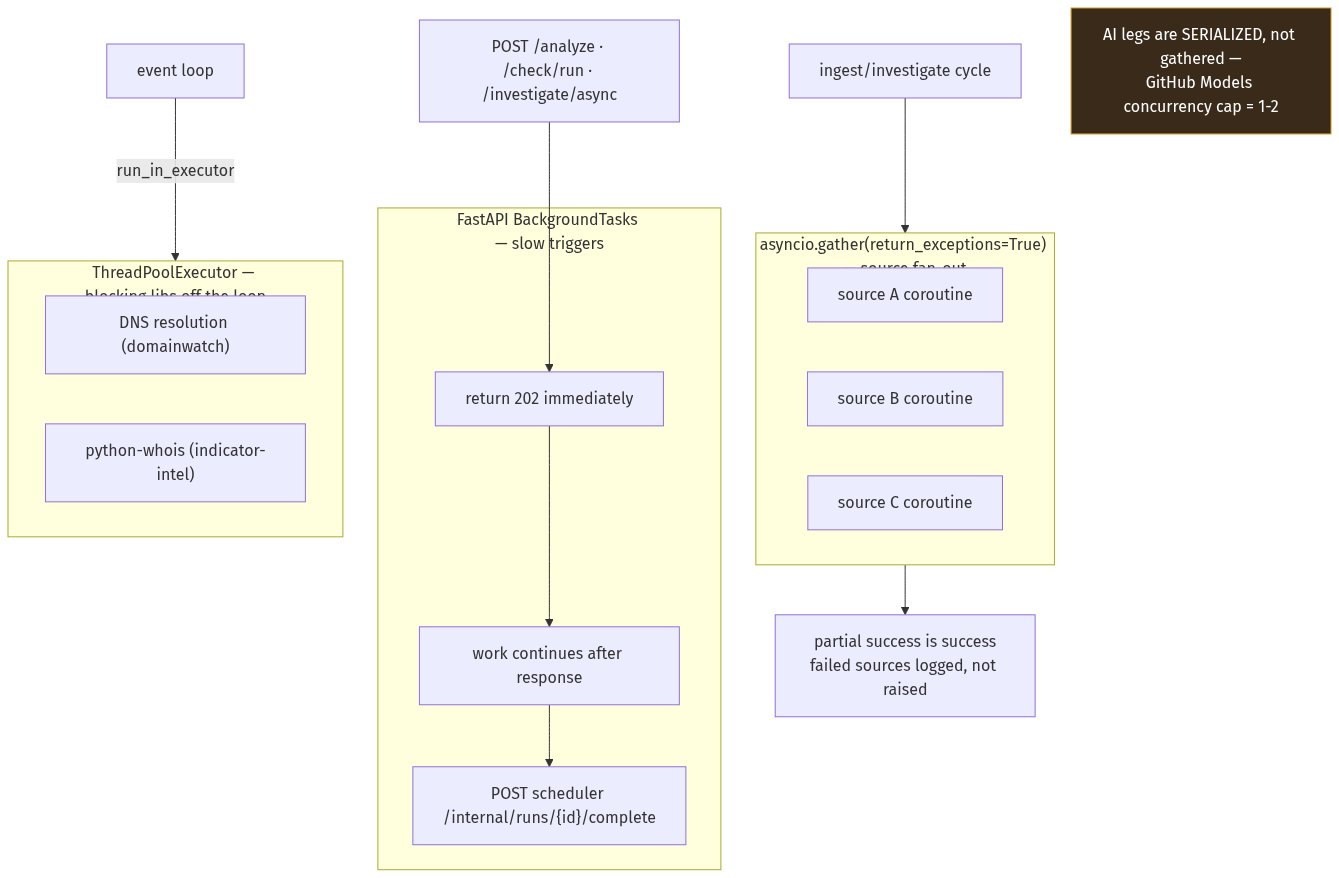
\includegraphics[width=0.92\textwidth]{images/tip/diagrams/10_async_execution.png}
\caption{Asynchronous execution patterns in the platform.}
\label{fig:async-new}
\end{figure}

\section{AI-Assisted Security Workflows}
AI is integrated into the platform as a bounded analytical layer rather than as a universal dependency.

This boundary is central to the implementation's soundness. AI systems are high-variance dependencies: they can fail, drift, hallucinate, or hit quota limits independently of the rest of the application. Treating them as ordinary synchronous business-logic calls would therefore contaminate ingestion, CRUD paths, and operator workflows with unnecessary volatility. By isolating AI behind a gateway and keeping it off the ingestion hot path, the implementation converts an unreliable external capability into a contained optional subsystem.

\subsection{Gatewayed AI Access}
All AI-capable services talk to a LiteLLM proxy instead of holding provider-specific credentials directly. This centralizes provider keys, creates one auditable outbound AI surface, and makes fallback routing a proxy concern rather than a per-service concern.

\subsection{Typed Structured Outputs}
AI calls that are expected to produce machine-usable results are validated against Pydantic schemas. This is one of the most technically mature aspects of the implementation. Instead of trusting a free-form string, the platform requests JSON-compatible outputs, validates them, and retries once on validation failure. The result is that orchestration code deals with typed objects rather than brittle prompt text.

The theoretical significance of this choice is larger than it first appears. It is an example of interface hardening. Instead of allowing a probabilistic model to define its own output format on each call, the application constrains the interaction contract. This reduces downstream ambiguity and makes it possible to distinguish three different failure classes clearly: provider failure, invalid structure, and semantically weak but structurally valid content. Only the last class still requires human review, which is exactly where it belongs.

\subsection{The Orchestrator Analysis Cycle}
The orchestrator performs a four-step cycle over already-ingested data: CVE relevance ranking, actor likelihood ranking, detection correlation, and executive briefing. A separate geo-prediction job runs on its own cadence. Each step persists outputs independently, which means one late-stage failure does not discard earlier successful analysis. This is a sound operational decision for quota-limited and failure-prone external model dependencies.

\subsection{Deep Indicator Investigation}
The indicator-intel service performs a more forensic-style workflow. It gathers context from passive and locally stored sources, performs dorking and enrichment, and returns a synthesized view rather than a single-source verdict. The feature is slower than the hot lookup path by design and is therefore architecturally separated from it.

This separation is conceptually important because it acknowledges two different temporal modes of security work. Triage requires speed and bounded latency. Investigation requires breadth and tolerates more delay in exchange for richer context. Trying to satisfy both with one endpoint often produces a poor compromise. The repository instead implements a dual-path design: a fast verdict path and a deeper enrichment path.

\section{Representative Features and Their Realization}
\subsection{The Dashboard}
The dashboard is not a static page backed by one service. It is powered by a frontend aggregation route that fans out to multiple backend services in parallel, then reshapes the result into one UI-oriented payload. This is a good use of the BFF pattern because it keeps composition logic close to the interface without forcing backend services to expose dashboard-specific payloads.

\begin{figure}[H]
\centering
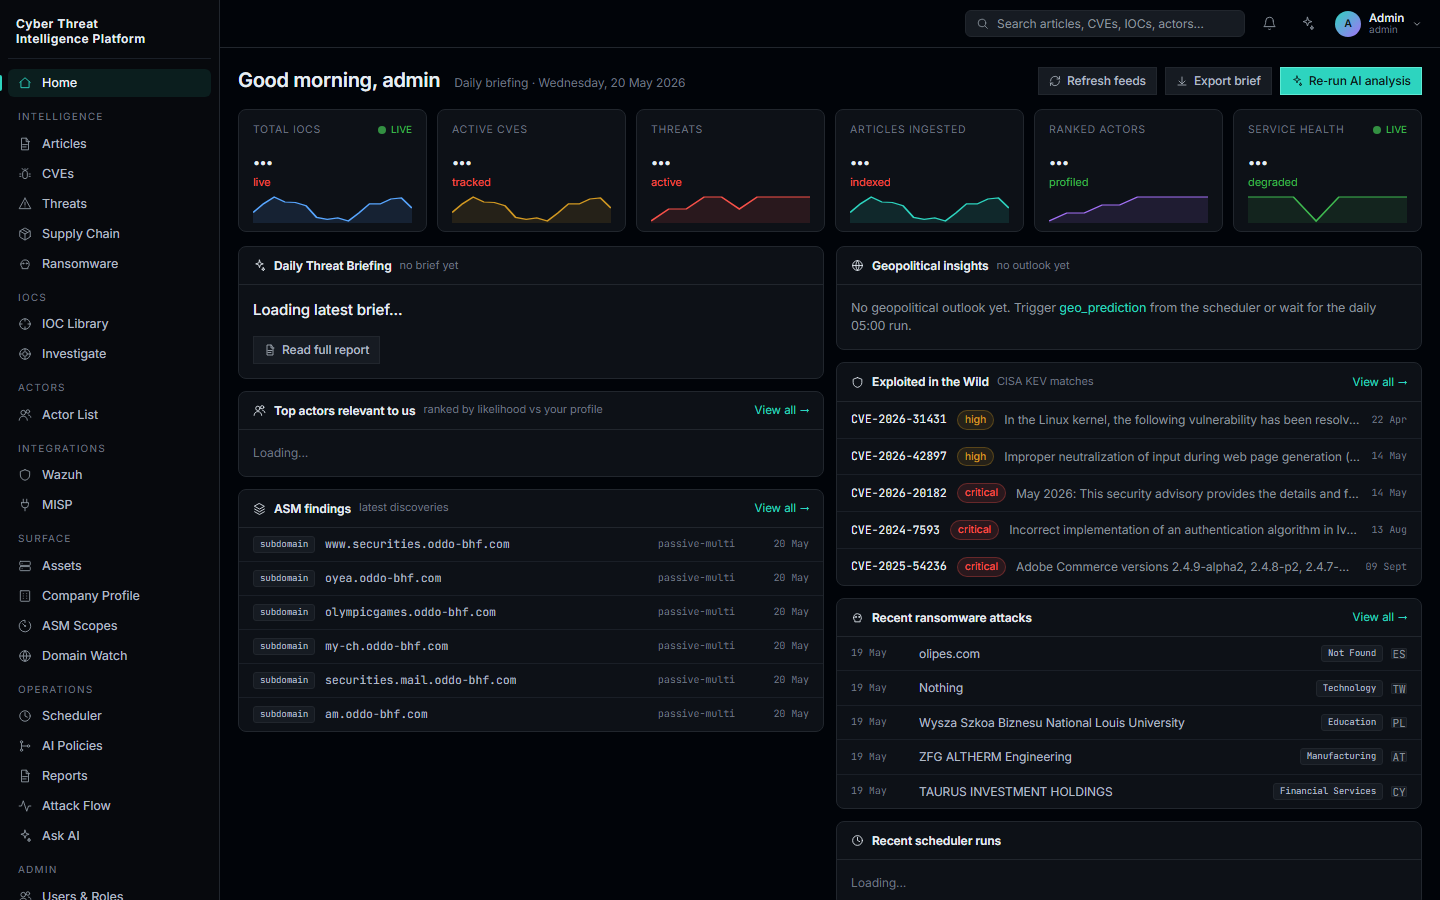
\includegraphics[width=0.95\textwidth]{images/tip/shots/02_dashboard.png}
\caption{Dashboard view assembled through the frontend aggregation route.}
\label{fig:dashboard-new}
\end{figure}

\subsection{IOC Lookup and Investigation}
The platform deliberately distinguishes between a sub-second lookup path and a slower investigation path. The first is optimized for triage and cache locality. The second is optimized for contextual depth.

\begin{figure}[H]
\centering
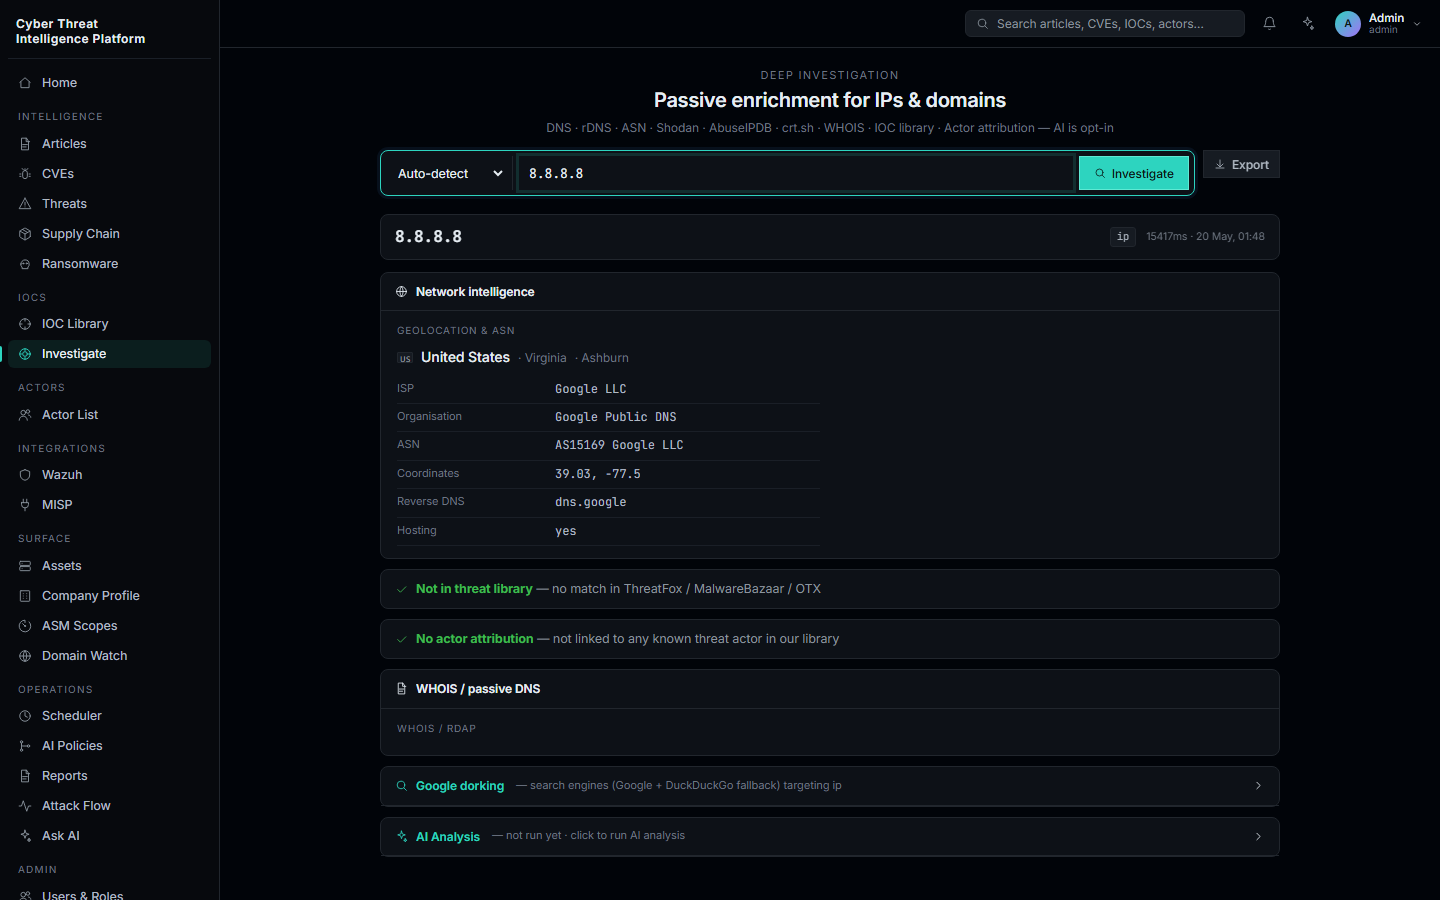
\includegraphics[width=0.95\textwidth]{images/tip/shots/16_ioc_investigate_result.png}
\caption{Indicator investigation result with multi-source enrichment.}
\label{fig:ioc-investigate-new}
\end{figure}

\subsection{Asset and Profile Context}
The CMDB service stores both assets and the company profile used by downstream synthesis. This is architecturally significant because it means vulnerability prioritization and actor ranking are not purely generic; they are conditioned on the organization's declared technologies, sectors, geographies, and threat concerns.

\begin{figure}[H]
\centering
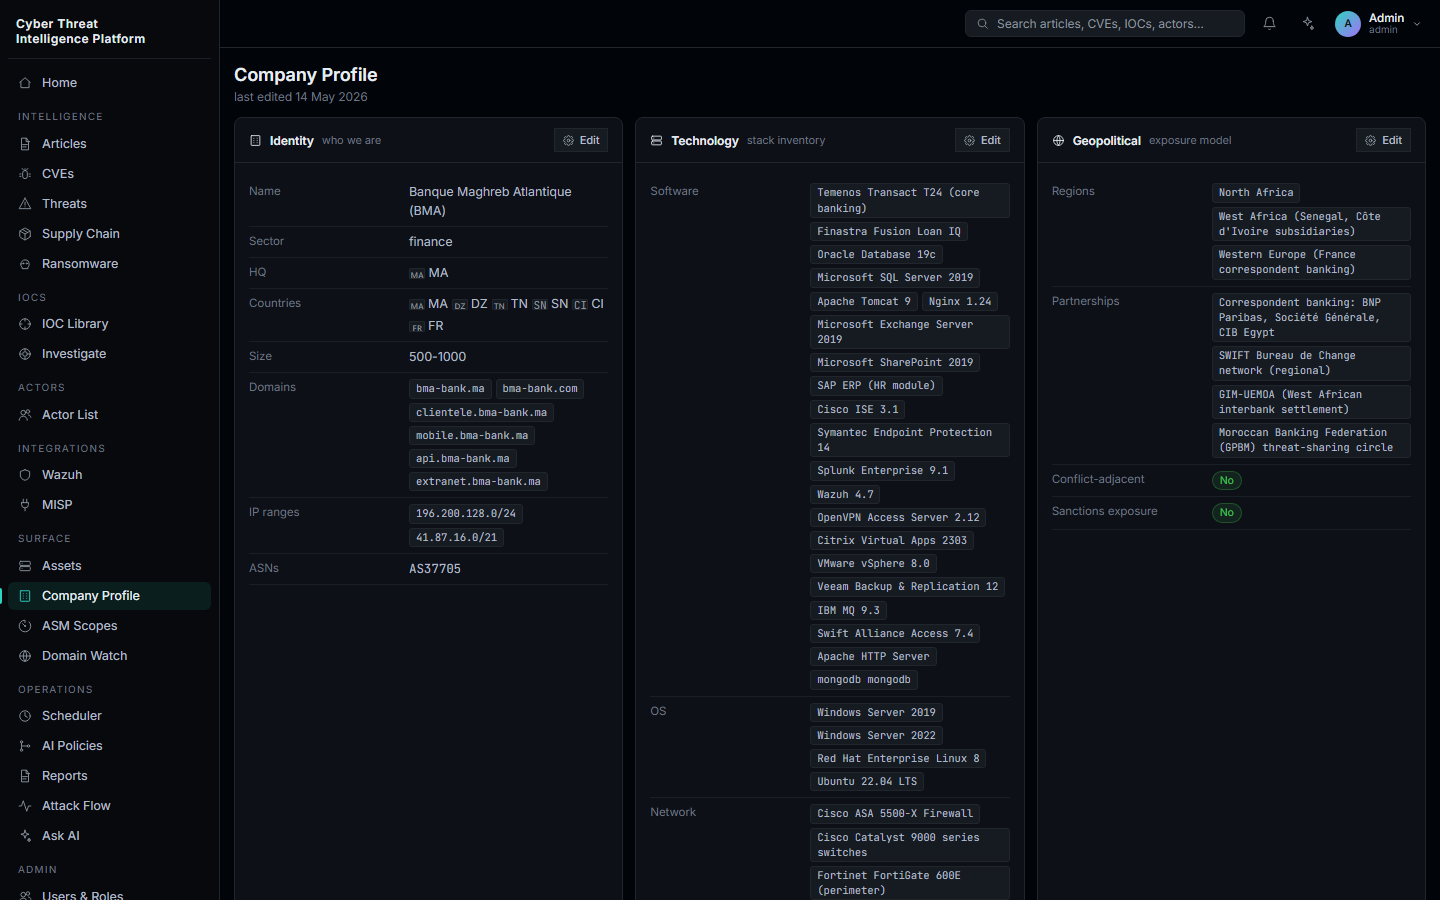
\includegraphics[width=0.95\textwidth]{images/tip/shots/23_assets_company_profile.png}
\caption{Company profile management in CMDB.}
\label{fig:company-profile-new}
\end{figure}

\subsection{Reports, Policies, and Flow Visualization}
Reports, AI policies, and generated attack flows give the system a managerial and analytical surface beyond simple list views.

\begin{figure}[H]
\centering
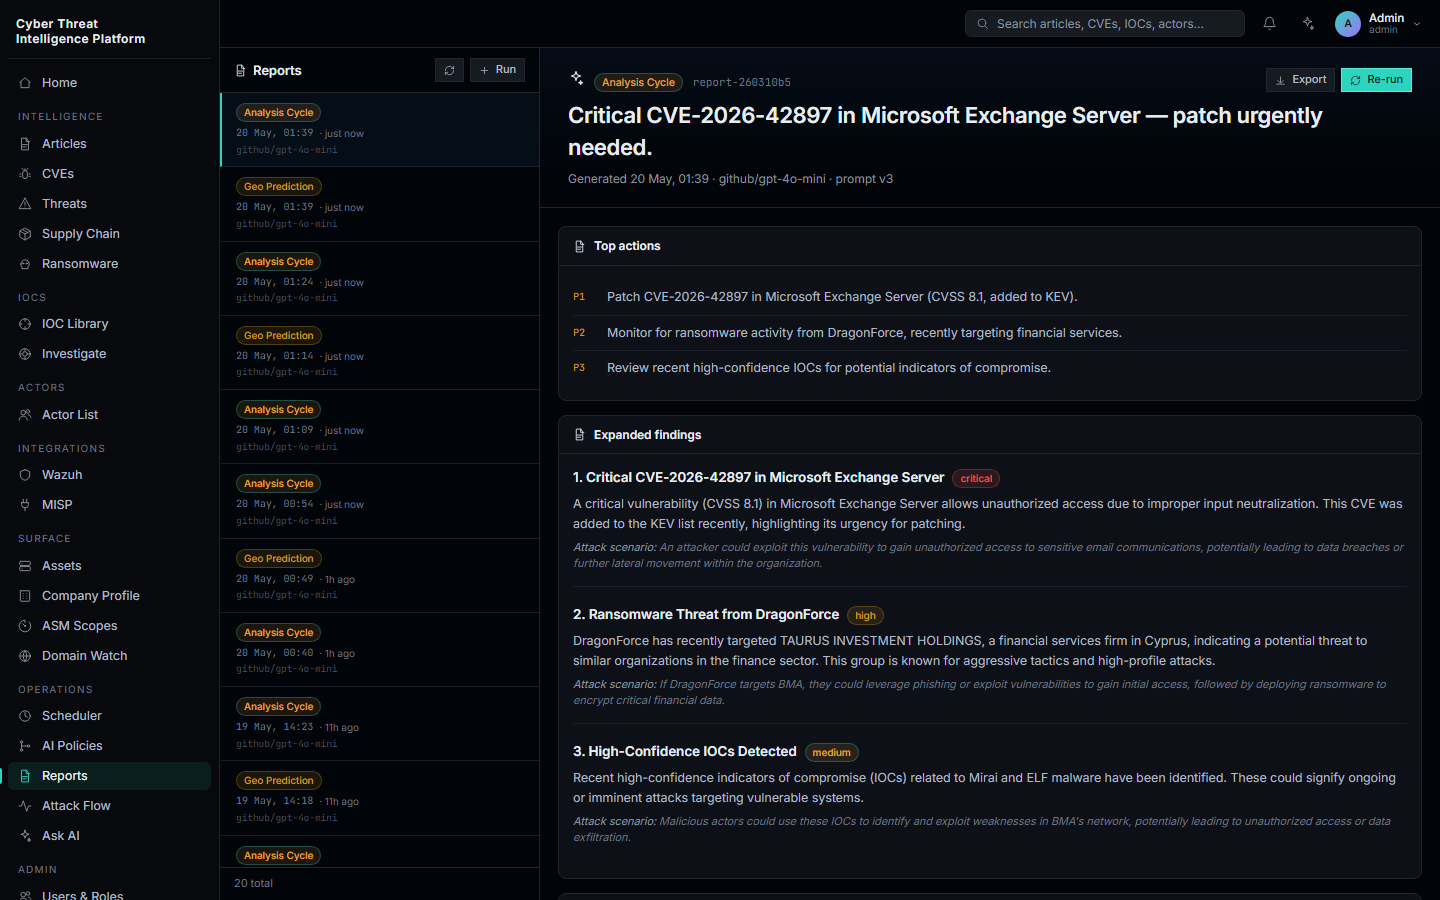
\includegraphics[width=0.95\textwidth]{images/tip/shots/31_reports.png}
\caption{Persisted report outputs generated by the orchestrator.}
\label{fig:reports-new}
\end{figure}

\begin{figure}[H]
\centering
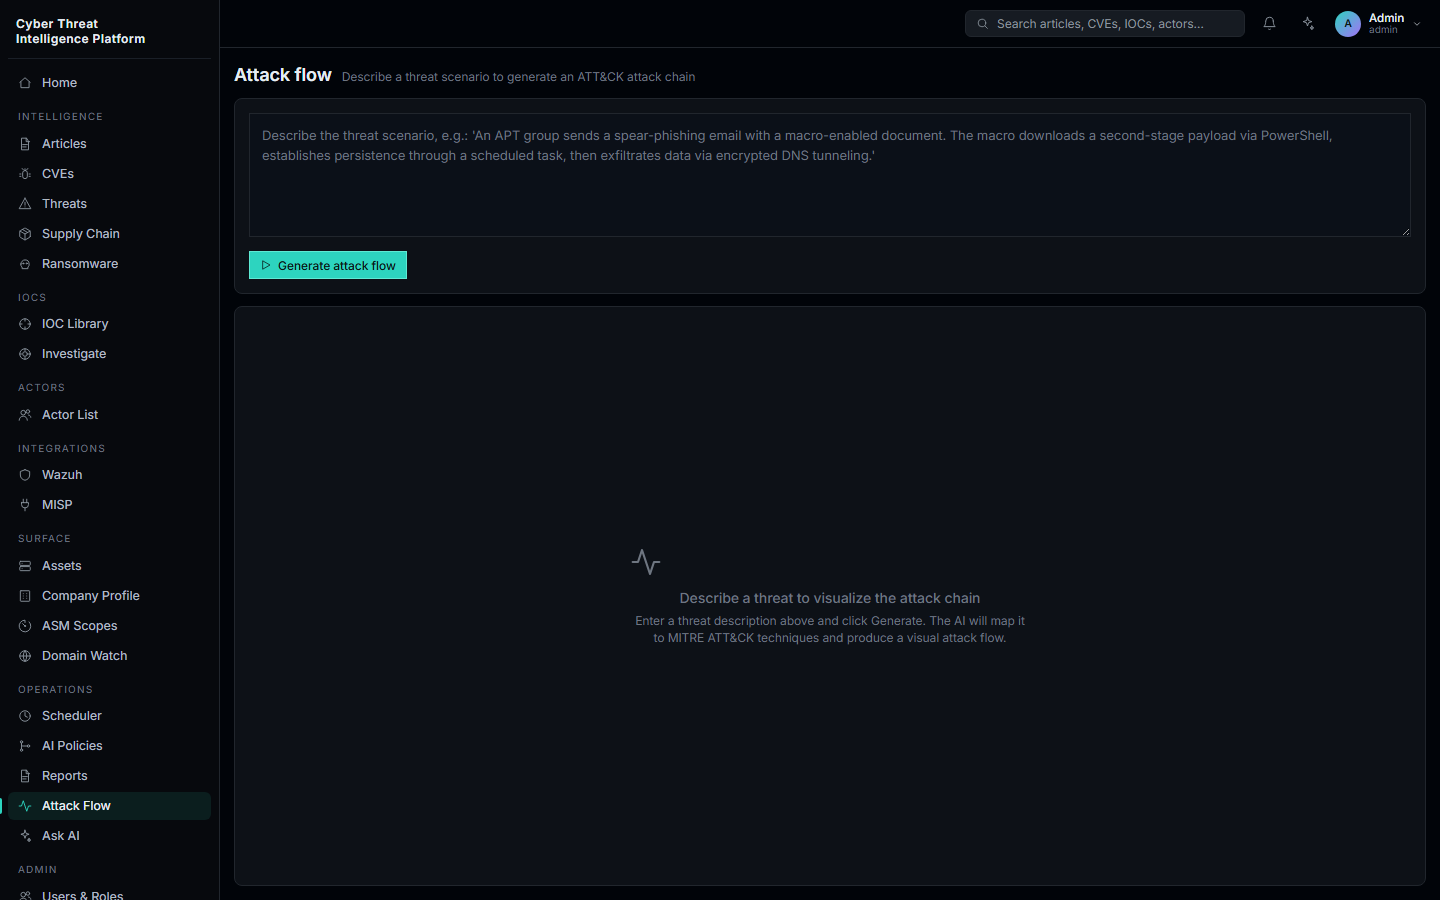
\includegraphics[width=0.95\textwidth]{images/tip/shots/33_flowviz.png}
\caption{Attack-flow visualization generated from structured analytical output.}
\label{fig:flowviz-new}
\end{figure}

\section{Containerization, Deployment, and Bootstrap}
Each service is packaged as its own image. This isolates dependencies and keeps rebuild scope bounded. The deployment topology is shown in Figures~\ref{fig:deploy-new} and \ref{fig:deploy-bottom}.

\begin{figure}[H]
\centering
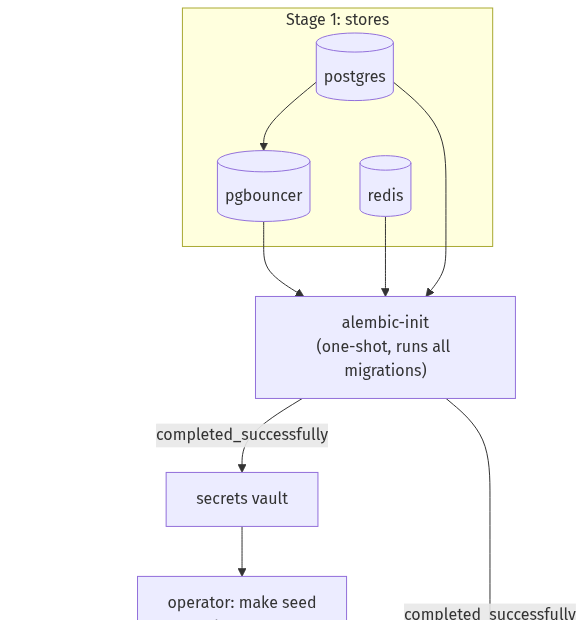
\includegraphics[width=0.72\textwidth]{images/tip/diagrams/05_deployment_topology_top.png}
\caption{Single-host deployment topology, startup and infrastructure segment.}
\label{fig:deploy-new}
\end{figure}

\begin{figure}[H]
\centering
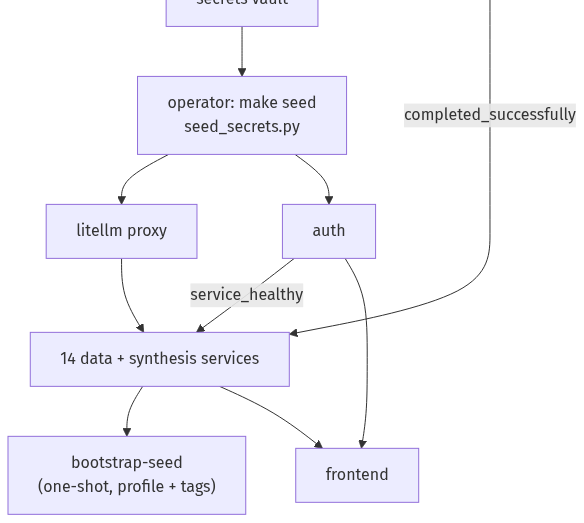
\includegraphics[width=0.72\textwidth]{images/tip/diagrams/05_deployment_topology_bottom.png}
\caption{Single-host deployment topology, service bring-up and application segment.}
\label{fig:deploy-bottom}
\end{figure}

The bootstrap sequence is intentionally ordered. Postgres, PgBouncer, and Redis start first. The one-shot migration container applies all Alembic migrations. The secrets service starts next, then auth and the LiteLLM proxy, followed by the remaining services. This ordering is enforced through Compose dependencies and health conditions rather than by manual sequencing.

This deployment choreography expresses an implicit dependency graph that exists whether it is documented or not. Databases must exist before migrations run. Secrets must exist before services can retrieve startup credentials. Authentication and key material must exist before some services can enforce request-time policy. Encoding this order explicitly in the deployment definition is an important implementation quality because it turns hidden operational knowledge into executable system behaviour.

\section{Observability, Logging, and Operator Diagnostics}
The observability model is pragmatic rather than elaborate. Each service exposes a health endpoint. Correlation IDs are propagated through middleware and bound into logs. Source-health tables show the last failure for upstream sources. Scheduler history records run state and duration. The secrets service records secret access. Together, these provide enough internal visibility for a small team to isolate common failure classes without requiring a full external telemetry stack.

Observability here should be understood as decision support for operators, not as telemetry maximalism. The goal is not to instrument every conceivable metric. The goal is to answer the kinds of questions that actually arise during failure: is the service alive, which upstream dependency is failing, which scheduled job is stuck, which secret was accessed, and which user-visible request produced the error chain in the logs. This focused notion of observability is well aligned with the platform's single-host operational model.

\section{Performance, Scalability, and Reliability}
\subsection{Performance Characteristics}
The platform is predominantly I/O bound. The main cost centres are database access, cache access, upstream feed calls, and AI inference. The most performance-sensitive path is IOC lookup, which is explicitly optimized with Redis. Other read paths favour correctness and stored-data access over aggressive caching.

\begin{figure}[H]
\centering
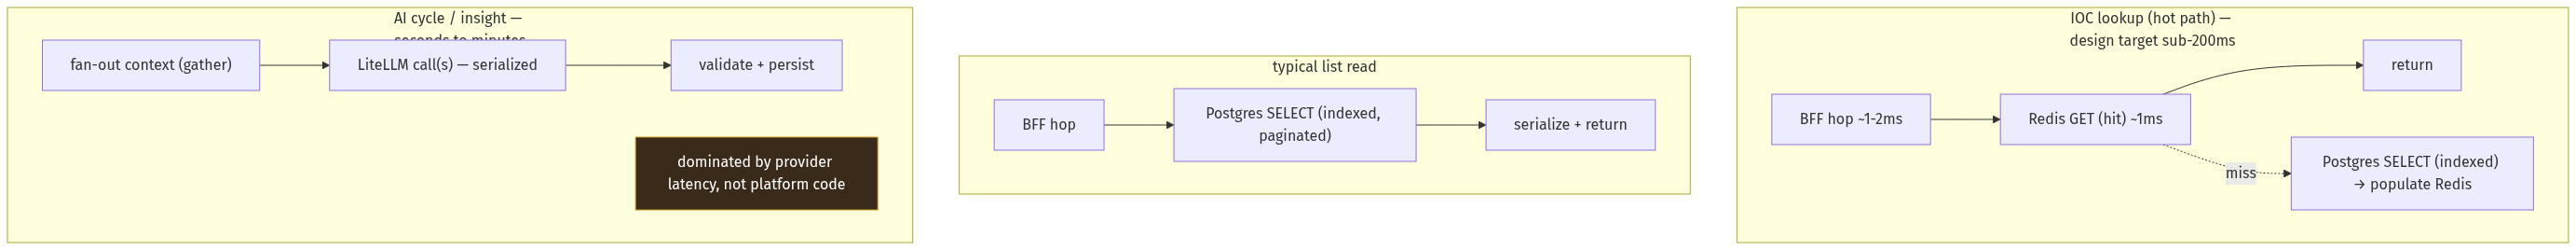
\includegraphics[width=0.9\textwidth]{images/tip/diagrams/13_latency_budget.png}
\caption{Qualitative latency budget by request class.}
\label{fig:latency-new}
\end{figure}

\subsection{Scalability Strategy}
The current deployment is single-host, but the codebase preserves several scale-friendly properties: stateless service processes, schema ownership, explicit service URLs, and isolation of AI, secrets, and scheduler concerns. Figure~\ref{fig:scaling-new} illustrates the intended scaling posture.

\begin{figure}[H]
\centering
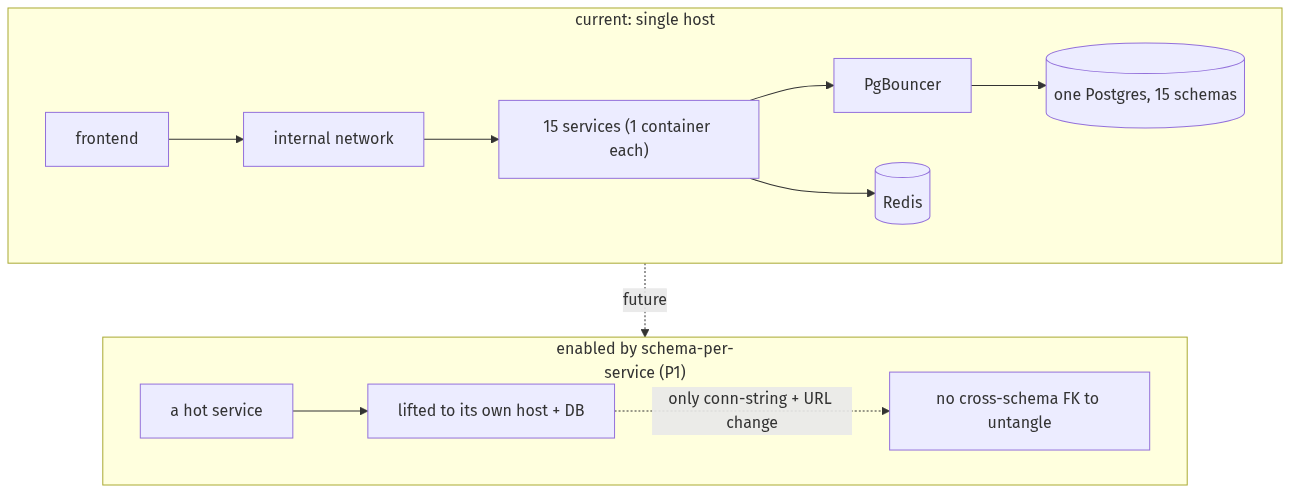
\includegraphics[width=0.9\textwidth]{images/tip/diagrams/13_scaling_model.png}
\caption{Current scaling posture and future expansion path.}
\label{fig:scaling-new}
\end{figure}

\subsection{Reliability Model}
Reliability is achieved primarily through graceful degradation, retryable source access, explicit source-health tracking, background task isolation, callback-driven scheduler semantics, and durable storage of analytical outputs. This is not a high-availability architecture in the strict sense, but it is a resilient single-host architecture.

That distinction between resilience and high availability should remain explicit. High availability concerns redundancy, failover, and continued service under infrastructure loss. Resilience concerns the ability to absorb partial dependency failure, recover predictably, and keep critical functions operating under degraded conditions. The implemented system is much stronger on the second axis than on the first, and the thesis should say so directly.

\section*{Conclusion}
\addcontentsline{toc}{section}{Conclusion}
The implementation translates architectural intent into a cohesive operating system for security analysis: consistent service construction, pooler-aware database access, resilient outbound HTTP, bounded AI integration, a real scheduler control plane, and an operator-facing interface that exposes the results. The strongest engineering choices are the separation of ingestion from synthesis, the disciplined use of shared packages, and the refusal to let AI sit on the platform's critical ingestion path. The next chapter addresses how this system is validated, where its testing posture is strong, where it is weak, and what limits remain.

\chapter{Verification, Security Testing, Limitations, and Future Work}
\thispagestyle{plain}
\section*{Introduction}
\addcontentsline{toc}{section}{Introduction}
This chapter evaluates the platform from the perspective of software assurance and operational maturity. It explains the real verification layers present in the repository, the gaps that remain, the security implications of current deployment choices, and the most credible next steps.

\section{Verification as an Engineering Discipline}
Verification should not be reduced to the question of whether unit tests exist. In software engineering, verification encompasses every mechanism used to establish that the implemented system conforms sufficiently to its intended behaviour, while validation addresses whether the right system was built for the problem at hand. Security platforms complicate this distinction because correctness is rarely exhausted by pure function-level logic. A system may be locally correct in code yet operationally weak if its deployment, trust boundaries, fallback behaviour, or failure visibility are poorly controlled.

For that reason, this chapter evaluates the platform across several verification layers: static correctness, runtime integration confidence, user-interface walkthroughs, security control review, and operational maturity. This broader view is necessary because the project's strongest properties are not located only in unit-level logic; they are also visible in its architecture, operator workflows, and degradation behaviour.

\section{Testing Strategy Overview}
The testing posture of the project must be described honestly. The repository does not contain a broad conventional unit and integration test suite. Instead, verification is weighted toward static analysis, smoke testing, manual end-to-end validation, and browser-driven walkthroughs. This is weaker than a mature CI-backed engineering baseline, but stronger than an unvalidated prototype.

This shape can be interpreted through the idea of a practical rather than idealized test pyramid. In a textbook pyramid, unit tests are numerous, integration tests fewer, and end-to-end tests relatively sparse. The project departs from that ideal because it was developed under tight scope and because many of its highest-risk behaviours lie at service boundaries, not only in pure internal functions. The resulting profile is therefore closer to an ``inverted'' or boundary-heavy strategy, where broad unit coverage is missing but real-stack and UI-level verification remain meaningful.

\begin{figure}[H]
\centering
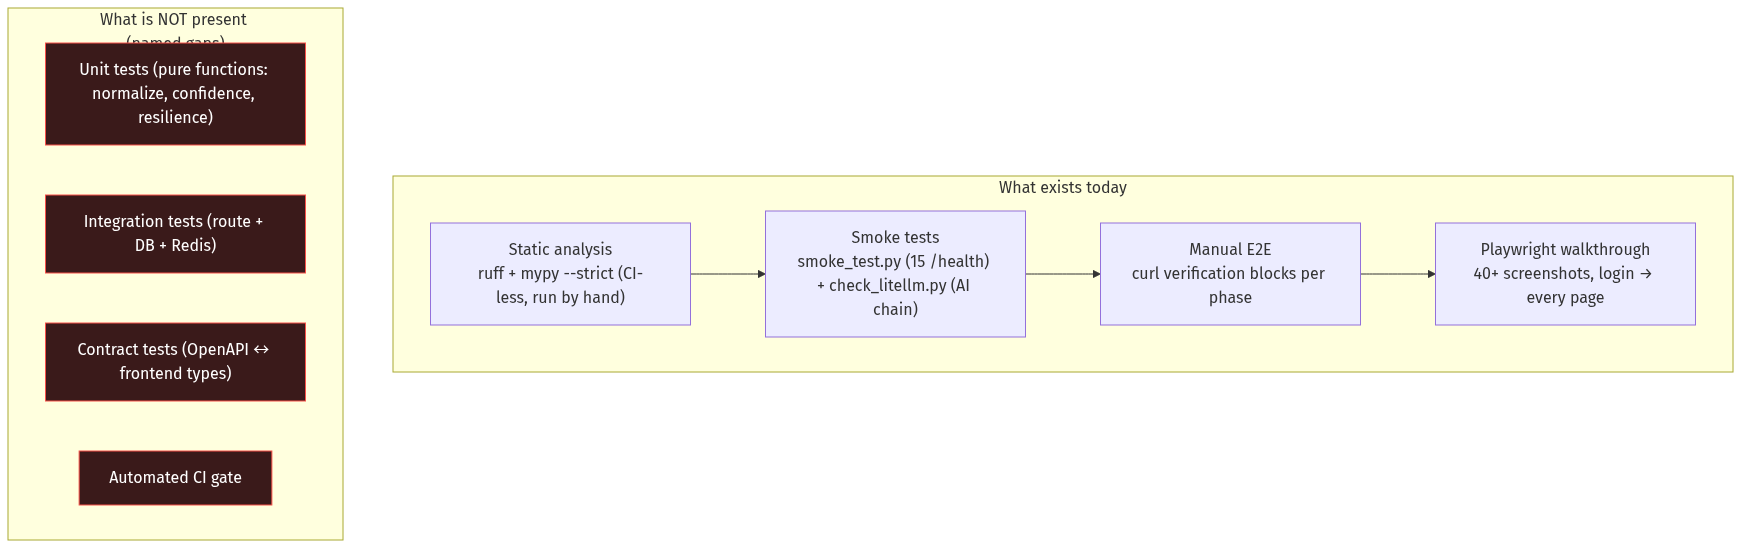
\includegraphics[width=0.85\textwidth]{images/tip/diagrams/11_test_strategy.png}
\caption{Verification strategy used by the project.}
\label{fig:test-strategy-new}
\end{figure}

\section{Unit Testing}
\subsection{Current State}
There is no substantive first-party unit test suite across the services and shared packages. This is an architectural and process limitation, not something that should be reframed as a hidden strength.

\subsection{What Is Indirectly Covered}
Some of the logic that would normally be exercised through unit tests is instead protected by static typing, validation models, and shared abstractions. The strict MyPy configuration and Ruff checks reduce type-level and API-shape regressions. Pydantic models catch many malformed inputs and schema mismatches. Shared helper functions reduce the amount of per-service duplicated logic that would otherwise need isolated tests.

Static analysis has particular value in this codebase because much of the platform's complexity lies in contract surfaces: typed settings, request and response schemas, service dependencies, and structured AI outputs. Type errors, shape mismatches, and inconsistent signatures are therefore not superficial issues. They are a large class of real defects that static tools can catch before runtime. This does not replace unit testing, but it does explain why static checks provide more defensive value here than they would in a loosely typed scripting codebase.

\subsection{What Should Be Unit Tested First}
If a unit test layer were added, the highest-value targets are clear: indicator normalization, confidence-score calculation, permission matching, scheduler callback helpers, secrets client fallback behaviour, AI response-shape validation, and risk or prioritization helpers that operate as pure logic.

\section{Integration Testing}
\subsection{Current State}
There is no broad automated integration suite that programmatically brings services together and validates inter-service contracts in a repeatable harness.

\subsection{What Exists Instead}
In practice, the repository relies on live-stack verification. Compose is used to stand up the full environment, migration and seed scripts create a usable state, and smoke tests verify service reachability. This approach gives higher-fidelity feedback on infrastructure wiring and service bootstrap, but weaker repeatability and lower isolation than a formal integration suite.

The theoretical strength of live-stack validation is environmental realism. It exercises the actual database, pooler, cache, container startup order, secret bootstrap, and inter-service routing topology. Its main weakness is reproducibility and automation depth. In other words, it is strong at catching integration reality and weak at supporting cheap regression frequency. That distinction is important because it shows the current verification posture is incomplete, not absent.

\section{End-to-End Testing with Playwright and Manual Walkthroughs}
The frontend and operational workflows are better covered than the backend unit layer. The repository contains a browser-driven walkthrough process that captures the UI surface and validates page-level navigation and rendering. The screenshots preserved in the LaTeX project are direct evidence of that process.

This style of validation is particularly useful for the frontend because the application depends on a BFF proxy, permission-sensitive navigation, authentication state, and cross-service aggregation routes. A narrow backend-only test would not catch many of the failure modes visible at the application boundary.

There is also a methodological point here. In systems where the frontend is a real integration boundary rather than a static veneer, browser-driven validation becomes more than cosmetic testing. It checks assumptions about authentication persistence, route aggregation, permission-gated navigation, latency tolerance, and the practical readability of outputs. Those are all part of system quality for an analyst-facing platform.

\section{Security Testing and Security Validation}
\subsection{Input and Schema Validation}
Request validation is strongly supported through FastAPI and Pydantic schemas. This gives consistent request-body parsing, query validation, and response typing across services.

\subsection{Authorization Validation}
Authorization intent is explicit in route dependencies. This makes missing permission checks visible in code review, even if the current deployment relaxes enforcement for many internal services.

\subsection{OWASP-Relevant Controls}
The platform implements several controls aligned with common web and API security guidance: role-based permissions, hashed passwords, hashed refresh tokens, centralized secrets, limited secret exposure through metadata-only listing, validation-driven request handling, and separation of public and bootstrap-only secret flows. However, the platform also carries real security debt: internal service auth is relaxed in Compose, provider access is centralized but still dependent on bootstrap secrets, and some backend ports are exposed directly.

Security verification in this context is therefore partly structural. Some claims can be supported by direct implementation evidence: passwords are hashed, refresh tokens are not stored in the clear, route dependencies make authorization intent visible, and secrets are centralized. Other claims require the opposite posture: they must be explicitly withheld because the implementation does not support them. This is why the thesis must discuss the softer internal trust boundary candidly rather than implying stronger guarantees than the runtime configuration actually provides.

\section{Performance Testing and Benchmarking}
There is no formal load-testing or benchmarking suite in the repository. Performance claims therefore need to remain bounded and honest. The strongest supported claim is architectural rather than numerical: the platform optimizes the hot IOC path, caches AI outputs to control cost and latency, uses PgBouncer to limit database pressure, and keeps ingest off the AI path so data freshness is not coupled to inference performance.

This chapter should therefore distinguish between performance design and performance proof. The repository clearly contains performance-aware design: hot-path caching, pooled connections, controlled fan-out, and bounded AI usage. What it does not yet contain is a formal measurement programme capable of turning those design intentions into rigorous throughput and latency claims. That gap belongs to future work, not to the current claim set.

\section{Verification Flow in Practice}
The de facto acceptance flow for changes is shown in Figures~\ref{fig:verify-new} and \ref{fig:verify-bottom}.

\begin{figure}[H]
\centering
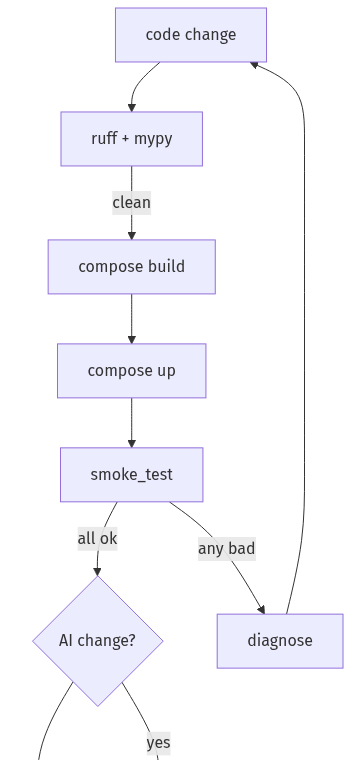
\includegraphics[width=0.5\textwidth]{images/tip/diagrams/11_verification_flow_top.png}
\caption{Manual verification flow used before accepting changes, upper segment.}
\label{fig:verify-new}
\end{figure}

\begin{figure}[H]
\centering
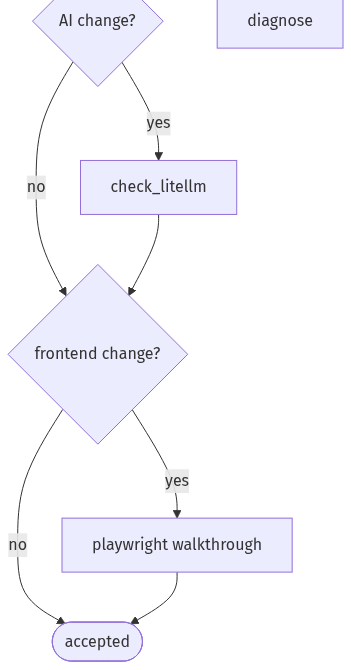
\includegraphics[width=0.5\textwidth]{images/tip/diagrams/11_verification_flow_bottom.png}
\caption{Manual verification flow used before accepting changes, lower segment.}
\label{fig:verify-bottom}
\end{figure}

This process is manual rather than CI-driven, but it is coherent. Static checks run first, followed by rebuild and recreate of impacted services, smoke testing, AI-chain testing when relevant, and browser walkthroughs for user-visible changes.

\section{Key Limitations}
\subsection{Testing Maturity}
The largest engineering gap is the absence of a broad automated unit and integration suite. The platform has meaningful verification, but it does not have the regression depth expected of a production-hardened multi-service system.

\subsection{Operational Hardening}
The platform runs on one host and does not yet implement an automated backup and recovery regime, formal CI/CD, or a richer metrics-and-alerting pipeline. These are classic day-two maturity gaps.

\subsection{Security Boundary Simplification}
Inter-service authentication is relaxed behind the Docker network for most services. This simplifies operation and avoids some service-to-service failure modes, but it creates a softer internal trust boundary than a stricter zero-trust design would provide.

\subsection{AI Dependence and Quota Sensitivity}
AI features are intentionally separated from ingestion, but the analytical layer remains dependent on external model providers and their quotas. The platform mitigates this through caching, fallback chains, and persistent output materialization, yet it does not eliminate the dependency.

Taken together, these limitations reveal a consistent maturity profile. The platform is relatively strong on domain modelling, service structure, contextual intelligence workflows, and bounded AI integration. It is weaker on automation depth, infrastructure redundancy, and formally measured non-functional proof. That is a normal profile for a successful PFE-scale engineering artefact, but it should remain explicit so the reader understands where the contribution genuinely lies.

\section{Future Work}
The most credible next steps are incremental rather than architectural rewrites.

\subsection{Testing Roadmap}
The highest-value improvement is to add unit tests around pure logic and integration tests around the most security-sensitive service boundaries, especially auth, secrets, scheduler callbacks, and orchestrator reporting.

\subsection{Operational Hardening}
Automated database backups, restore drills, CI/CD gates, and metrics-backed alerting should follow soon after. These changes improve reliability without requiring a fundamental redesign.

\subsection{Security Hardening}
A production-grade evolution of the platform should re-enable and validate inter-service auth selectively, reduce direct exposure of non-frontend service ports, and strengthen bootstrap-token handling and rotation.

\subsection{Scalability Evolution}
The schema-per-service design and explicit service URLs make it feasible to move the heaviest services or stores onto separate hosts later, but that should follow operational hardening rather than precede it.

\chapter*{General Conclusion}
\addcontentsline{toc}{chapter}{General Conclusion}
The implemented Threat Intelligence Platform responds to a concrete operational problem: a security team working under modern threat pressure cannot afford to manually assemble context from disconnected feeds, vulnerability sources, indicator stores, actor libraries, and internal tooling every time it needs to make a triage or prioritization decision. The system addresses that problem by combining continuous ingestion, deterministic normalization, organization-aware prioritization, structured AI-assisted synthesis, and a user interface that makes those outputs operationally usable.

From an architectural perspective, the strongest aspects of the platform are its disciplined service ownership model, its clear separation between ingest and synthesis, its shared service skeleton, its centralized secret handling, and its practical use of a BFF proxy and scheduler control plane. From an operational perspective, its main value lies in turning raw threat information into a ranked and contextualized decision surface without forcing the team to depend on many separate tools.

The platform is also notable for what it does not pretend to be. It is not yet a highly available distributed system. It does not have mature automated test depth. It does not claim strict zero-trust internal segmentation in its current Compose deployment. These are real limitations, but they do not undermine the core contribution of the work. They show that the system is a technically coherent and operationally credible platform whose remaining gaps lie mainly in hardening, automation, and production engineering maturity rather than in basic design.

The most important result is therefore not only that the platform works, but that its internal structure makes improvement tractable. Testing can be deepened without redesign. Stronger service-to-service auth can be reintroduced without abandoning the current service model. Operational safeguards such as backup automation, CI/CD, and richer observability can be added incrementally. That combination of functional completeness, explicit tradeoffs, and credible upgrade paths is what makes the system thesis-worthy as an engineering artefact.


%%%%%%%%%%%%%%%%%%%%%%%%%%%%%%%%%%%%%%%%%%%%%%%%%%%%%%%%%%%%%%%%%%%%%%%%%%%%%%%%%%%%%%%%%%
\cleardoublepage
\phantomsection
\addcontentsline{toc}{chapter}{Webography}

\nocite{*}
\printbibliography


%%%%%%%%%%%%%%%%%%%%%%%%%%%%%%%%%%%%%%%%%%%%%%%%%%%%%%%%%%%%%%%%%%%%%%%%%%%%%%%%%%%%%%%%%%

% Abstract and Résumé stacked vertically - for inclusion in main document
\cleardoublepage
\phantomsection

\thispagestyle{empty}

\vspace*{\fill}

\noindent
\begin{tabular}{|p{0.94\textwidth}|}
\hline
\\[0.6em]
\multicolumn{1}{|c|}{\textbf{\large Abstract}} \\[0.5em]
Modern security teams operate under compressed decision windows shaped by fast exploitation, identity-led intrusion, supply-chain compromise, and AI-assisted offensive tradecraft. Intelligence is abundant, but it is fragmented across feeds, tooling, and operational systems, which makes contextual prioritization slow and inconsistent.

\vspace{0.5em}
This project presents a self-hosted Threat Intelligence Platform built as fifteen cooperating FastAPI services over a schema-partitioned PostgreSQL database, with Redis, PgBouncer, a Next.js frontend, and a LiteLLM gateway. The platform continuously ingests intelligence from external sources, normalizes and deduplicates it, enriches it with organizational context, and applies structured AI-assisted analysis to produce ranked vulnerabilities, likely threat actors, operational reports, and analyst-facing investigation outputs.

\vspace{0.5em}
The analytical layer reads only processed data and never blocks ingestion, so the platform keeps operating when upstream AI providers fail. Services are isolated by schema, external calls are wrapped in a resilience layer, secrets are centralized, and the system remains operable on a single host. The report also evaluates the platform honestly: strong modularity and useful analytical acceleration are balanced against limited automated testing, a simplified internal trust model, and remaining production-hardening work.

\vspace{0.5em}
\textbf{Keywords:} Threat Intelligence, Microservices, Cybersecurity, Large Language Models, Fault Tolerance, API-First Architecture
\hline
\\[0.6em]
\multicolumn{1}{|c|}{\textbf{\large Résumé}} \\[0.5em]
Les équipes de sécurité opèrent aujourd'hui sous une forte compression du temps de décision, alimentée par l'exploitation rapide des vulnérabilités, la compromission des identités, les attaques de la chaîne d'approvisionnement et l'usage offensif de l'intelligence artificielle. Le renseignement existe en abondance, mais il reste dispersé entre de multiples flux et outils, ce qui rend la priorisation contextuelle lente et incohérente.

\vspace{0.5em}
Ce projet présente une plateforme de renseignement sur les menaces auto-hébergée, construite sous la forme de quinze services FastAPI coopérants autour d'une base PostgreSQL partitionnée par schéma, avec Redis, PgBouncer, une interface Next.js et une passerelle LiteLLM. La plateforme ingère en continu des renseignements provenant de sources externes, les normalise et les dédoublonne, les enrichit avec le contexte de l'organisation, puis applique une analyse assistée par l'IA pour produire des vulnérabilités classées, des acteurs probables, des rapports opérationnels et des résultats d'investigation pour les analystes.

\vspace{0.5em}
La couche analytique ne lit que des données déjà traitées et ne bloque jamais l'ingestion, ce qui permet à la plateforme de continuer à fonctionner même en cas de défaillance d'un fournisseur d'IA. Les services sont isolés par schéma, les appels externes sont rendus résilients, les secrets sont centralisés, et le système reste exploitable sur un hôte unique. Le mémoire évalue aussi honnêtement les limites actuelles : tests automatisés encore insuffisants, modèle de confiance interne simplifié et travaux de durcissement encore nécessaires.

\vspace{0.5em}
\textbf{Mots-clés :} Renseignement sur les menaces, Microservices, Cybersécurité, Modèles de langage, Tolérance aux pannes, Architecture orientée API
\\[0.6em]
\hline
\end{tabular}

\vspace*{\fill}

\end{document}
